\chapter{Calorimeter Optimisation Studies}
\label{chap:detopt}

\chapterquote{There, sir! that is the perfection of vessels!}
{Jules Verne, 1828--1905}

%========================================================================================
%========================================================================================

\section{Calorimeter Optimisation Studies}
If the future linear collider is to reach it's maximum potential in terms of energy resolution then, optimisation of the detector will be essential.  The energy resolution in the particle flow paradigm is dependant upon several detector components.  The momentum of charged particles arises from the shape of the tracks deposited within the detector while the energy of uncharged particles arise from calorimetric measurements.  Application of sophisticated pattern recognition algorithms allows the particle type to be inferred for the charged particles.  In tern this allows for the conversion of the track momentum into an energy measure for the charged particles.  The particle identification algorithms use the topological information acquired from the calorimetric energy deposited to infer particle type for a subset of charged particles.  

The calorimetric energy deposits are therefore used in a twofold manner: (i) as energy measurements for neutral particles and (ii) as input for particle identification algorithms.  There is potential for significant gains to be made in physics performance by optimising the calorimeters due to their dominant role in energy measurements.  In this chapter the optimisation of the calorimeters is considered.  Parameters such as the longitudinal granularity, transverse granularity and material choices for the calorimeters are considered.  

This chapter concludes with an optimisation of several global parameters for the detector.  These parameters are not calorimeter specific, but the optimisation procedure developed for the calorimeters is appropriate to use.  These parameters relate to the global detector size and the magnetic field applied throughout solenoid in the detector.

%========================================================================================
%========================================================================================

\section{Metric}

%========================================================================================
%========================================================================================

\section{Simulation and Reconstruction}

%========================================================================================
%========================================================================================

\section{Calibration}

\section{Nominal Detector Performance}
The energy resolution for single photon events as a function of photon energy, for the nominal ILD detector, is shown in figure \ref{fig:ecalnominalres}.  The nominal jet energy resolution can be found in section BLAH.

\begin{figure}
\centering
\subfloat[Silicon active material, $5 \times 5 \text{mm}^{2}$ ECal transverse granularity.]{\label{fig:ecalsinominalres}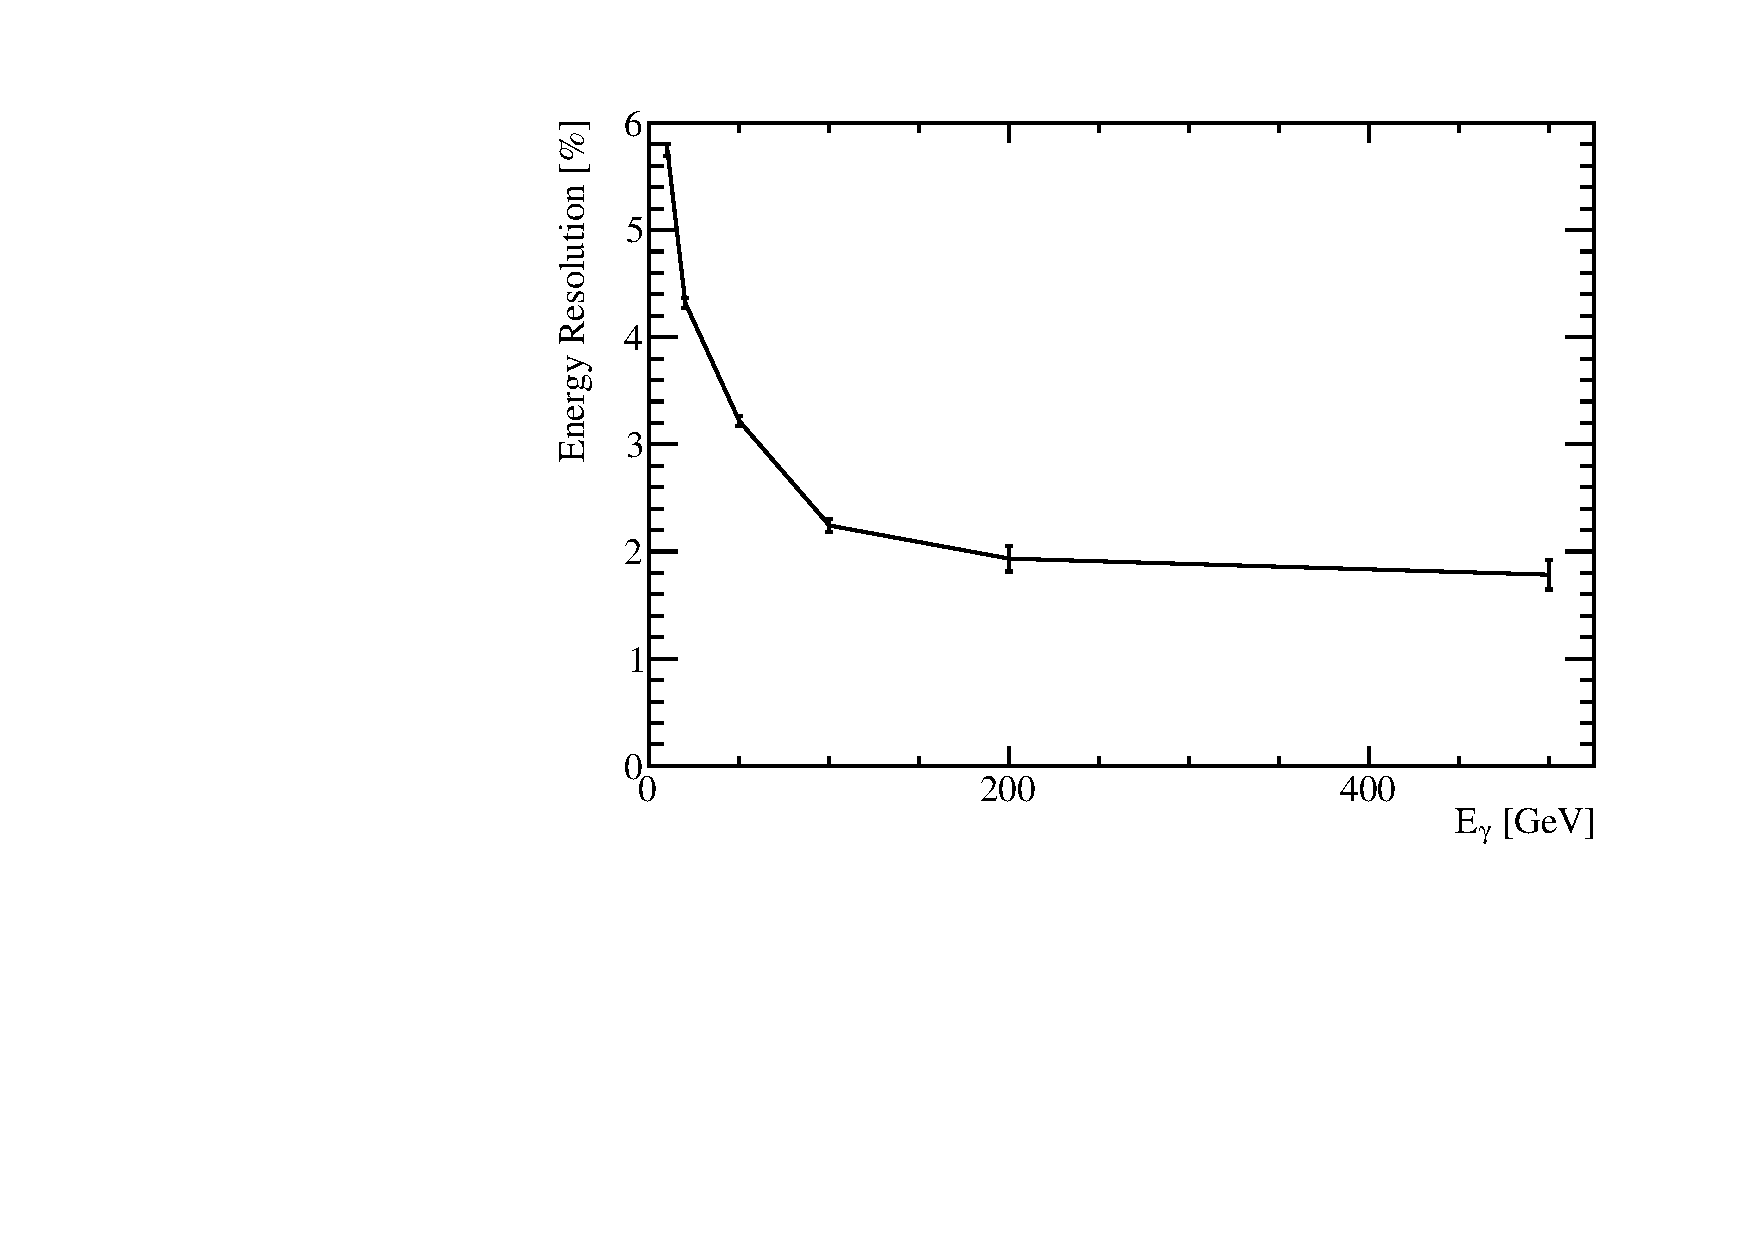
\includegraphics[width=0.5\textwidth]{OptimisationStudies/Plots/EnergyResolution/ER_vs_EGamma_SiliconECal.pdf}}
\subfloat[Scintillator active material, $5 \times 5 \text{mm}^{2}$ ECal transverse granularity.]{\label{fig:ecalscnominalres}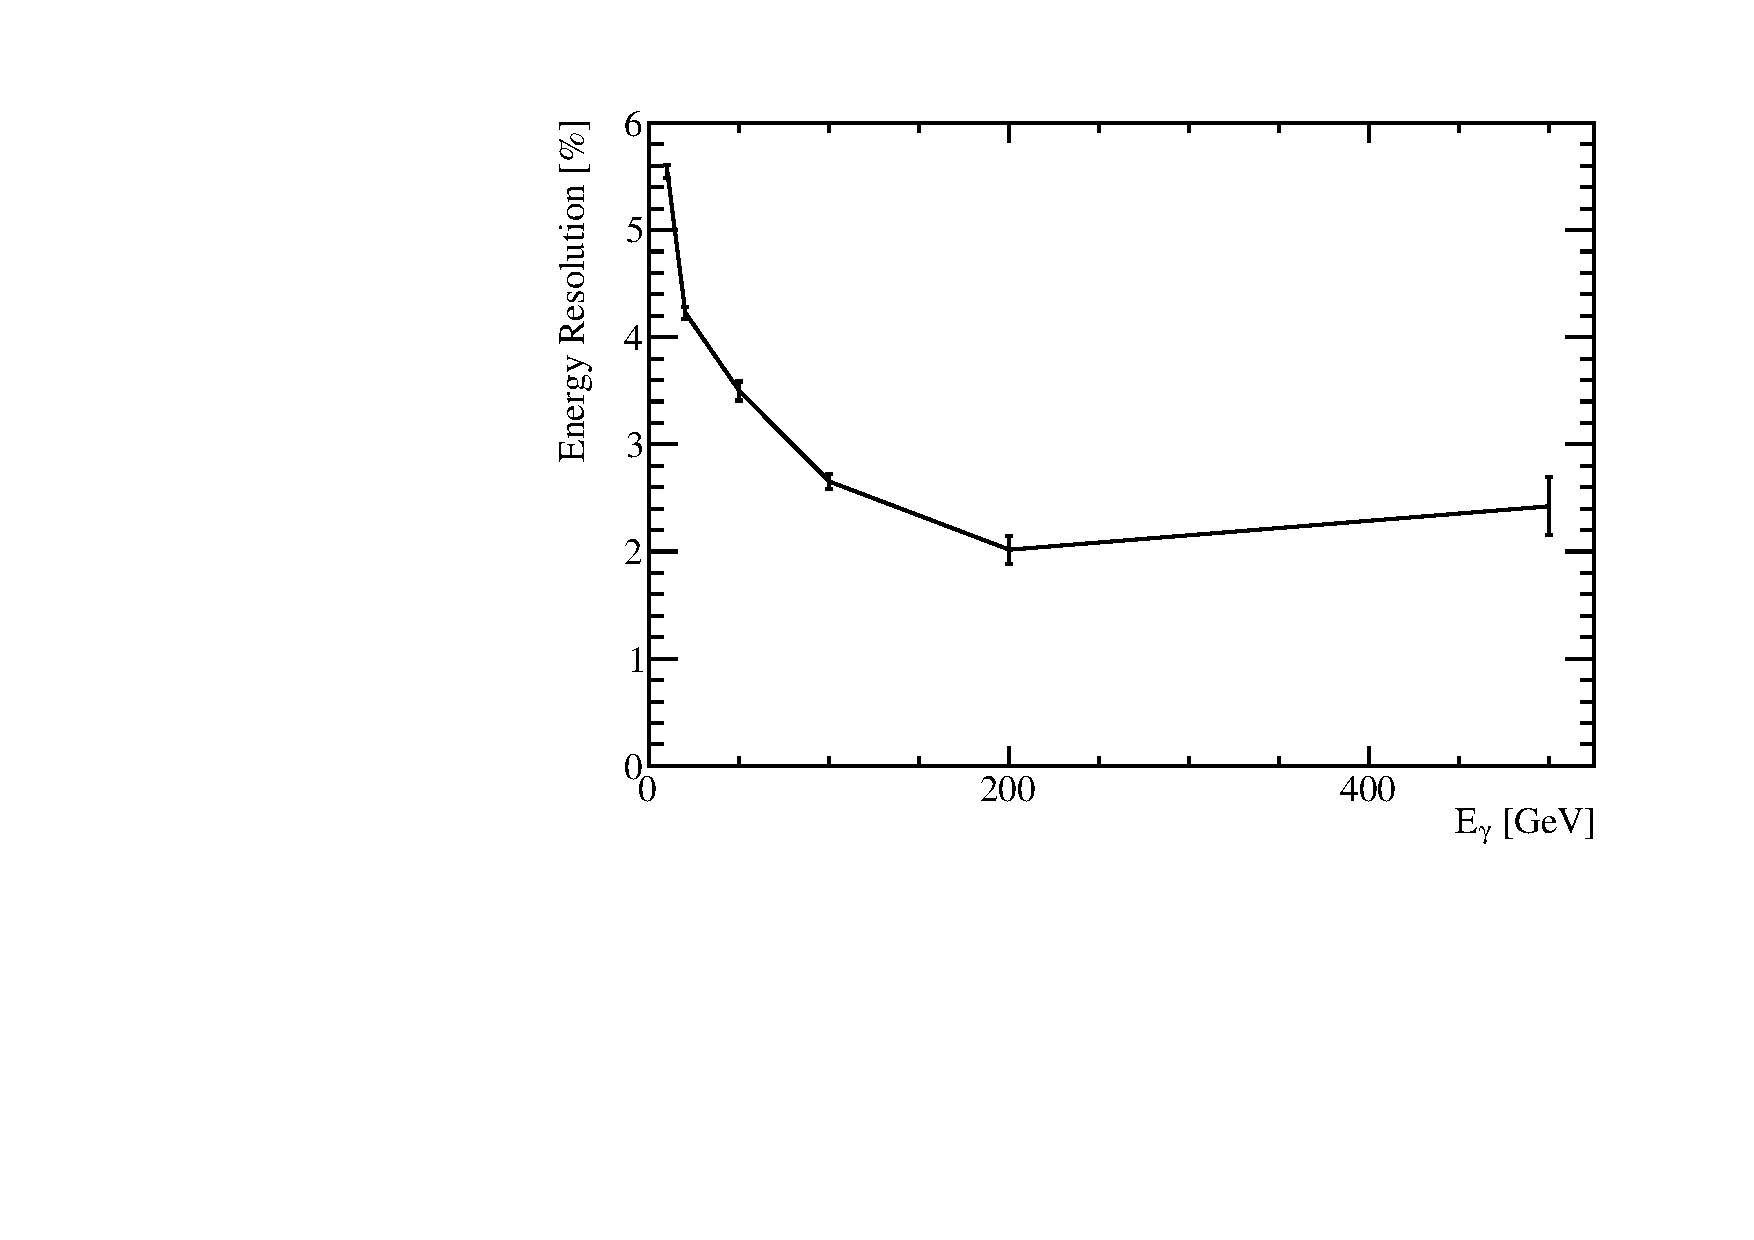
\includegraphics[width=0.5\textwidth]{OptimisationStudies/Plots/EnergyResolution/ER_vs_EGamma_ScintillatorECal.pdf}}
\caption[Energy resolution as a function of photon energy for the nominal ILD detector for both the silicon and scintillator options.]{Energy resolution as a function of photon energy for the nominal ILD detector for both the silicon and scintillator options.}
\label{fig:ecalnominalres}
\end{figure}

%========================================================================================
%========================================================================================

\section{Electromagnetic Calorimeter Optimisation}
\label{sec:ecal}
The ECal primarily measures the energy deposits of electromagnetic showers.  The default ILD detector model ECal, summarised in table \ref{table:defaultildecal}, contains 24 radiation lengths ($\text{X}_{0}$, which acts to confine all but the highest energy electromagnetic showers within it.  The longitudinal structure of this default model is 29 readout layers, consisting of pairs of active and absorber material, and one presampling layer, which exists to encourage shower development.  Increasing the thickness of the absorber material part way into the detector reduces the number of readout channels and cost of the overall calorimeter while retaining a high sampling rate at the start of particle showers, which is crucial for the pattern recognition aspect of particle flow calorimetry.  

\begin{table}[h!]
\centering
\begin{tabular}{ l l}
\hline
Parameter & Default Value \\
\hline
Transverse Granularity & $5 \times 5 \text{mm}^{2}$ square cells \\
Longitudinal Granularity & 29 Readout Layers, 1 Presampling Layers \\
Active Material Choice & Silicon or Scintillator  \\
Active Material Thickness & 0.5 mm (Silicon) or 2 mm (Scintillator)  \\
Absorber Material Choice & Tungsten \\
Absorber Material Thickness & 20 Layers of 2.1 mm followed by 9 Layers of 4.2 mm \\
\hline
\end{tabular}
\caption[Nominal ILD detector model ECal configuration.]{Nominal ILD detector model ECal configuration.}
\label{table:defaultildecal}
\end{table}

The parameters being optimised in this study are:
\begin{itemize}
\item Transverse granularity or cell size.  This is a vital aspect of the detector in the particle flow paradigm as smaller cell sizes give greater potential for being able to separate energy deposits from charged and neutral particles.  This transverse granularity should have little to no effect on the intrinsic energy resolution of the detector.  
\item Longitudinal granularity or cell depth.  This parameter dictates the intrinsic energy resolution of the detector as smaller cell depths mean more sampling is done of the particle shower and so, due to the Poissonian statistics governing the measurement of particle showers, the better the resolution.
\item Active material choice.  This is a choice between silicon or scintillator.  As well as providing different intrinsic energy resolutions the readout mechanics of these two options are significantly different.  There is no clear prior knowledge as to which should provide better performance. 
\end{itemize}

%========================================================================================

\subsection{ECal Transverse Granularity}
\label{sec:ecalcells}
For this study a number of different detector models were considered where the transverse granularity in the ECal had been varied about the nominal value of $5 \times 5 \text{mm}^{2}$ square cells.  The granularities considered were $3 \times 3 \text{mm}^{2}$, $5 \times 5 \text{mm}^{2}$, $7 \times 7 \text{mm}^{2}$, $10 \times 10 \text{mm}^{2}$, $15 \times 15 \text{mm}^{2}$ and $20 \times 20 \text{mm}^{2}$ square cells for both the silicon and scintillator active material options.  The jet energy resolution as a function of transverse granularity in the ECal is shown in figure \ref{fig:ecalcellsize}.

\begin{figure}
\centering
\subfloat[Silicon active material.]{\label{fig:ecalsicellsize}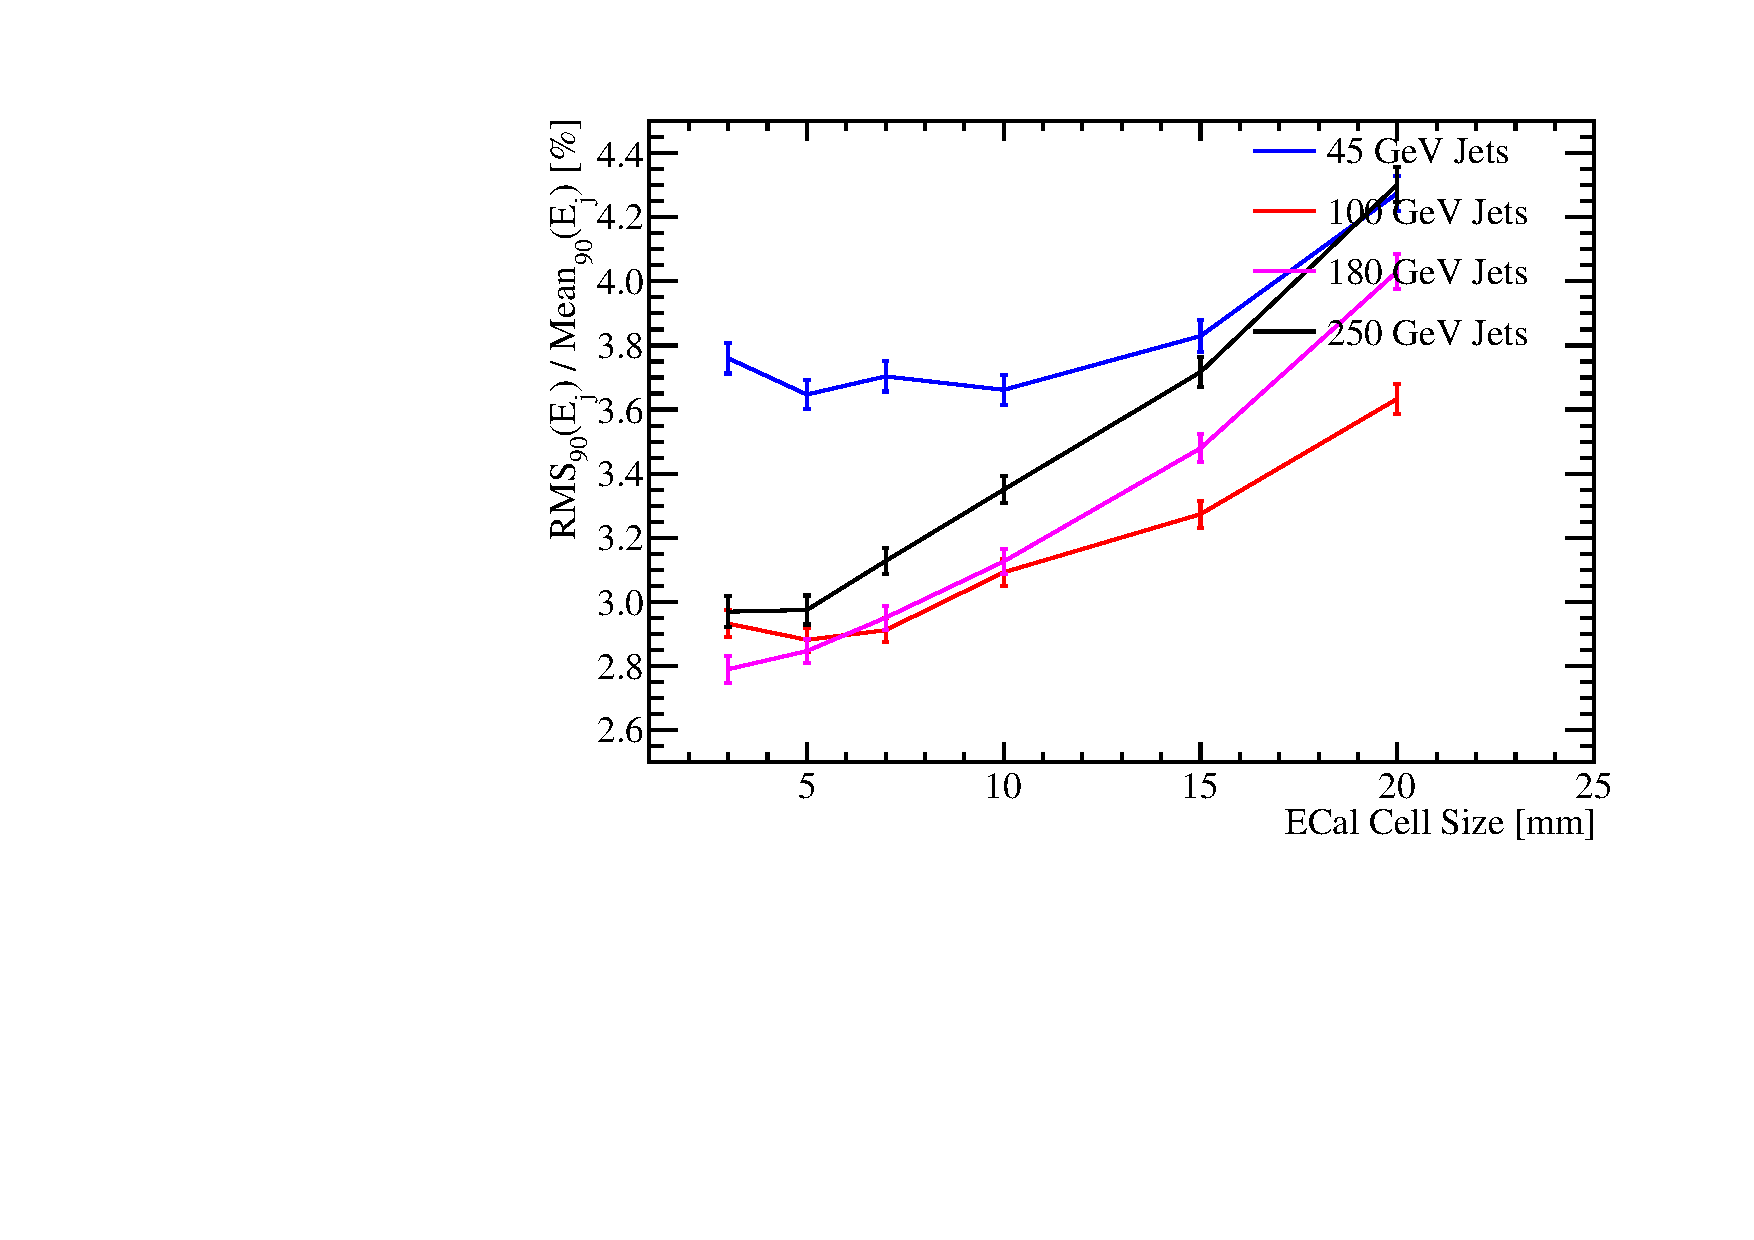
\includegraphics[width=0.5\textwidth]{OptimisationStudies/Plots/JetEnergyResolutions/JER_vs_SiliconECalCellSize.pdf}}
\subfloat[Scintillator active material.]{\label{fig:ecalsccellsize}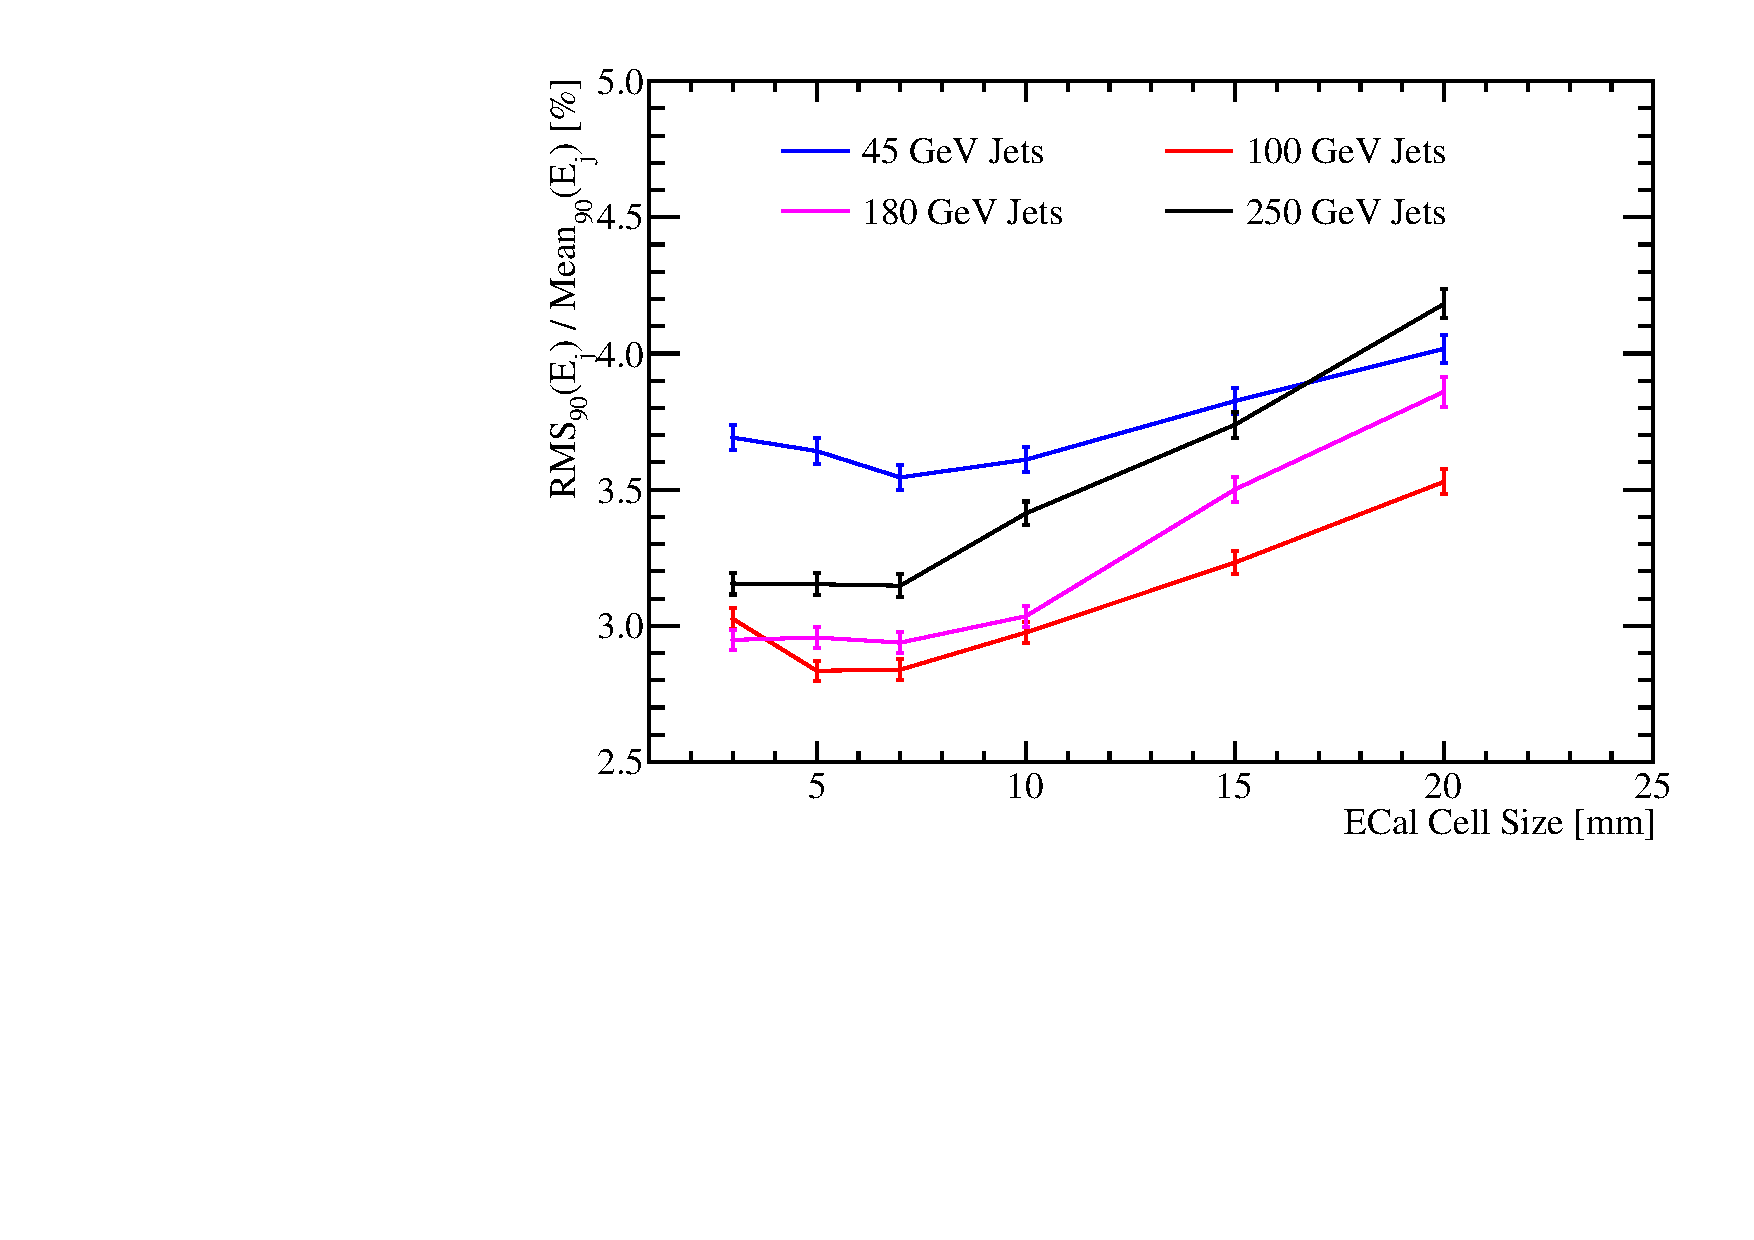
\includegraphics[width=0.5\textwidth]{OptimisationStudies/Plots/JetEnergyResolutions/JER_vs_ScintillatorECalCellSize.pdf}} \hfill
\caption[Jet energy resolution as a function of ECal cell size.]{Jet energy resolution as a function of ECal cell size for the silicon and scintillator ECal options.}
\label{fig:ecalcellsize}
\end{figure}

The jet energy resolution was found to improve with decreasing cell size.  This is expected as smaller cell size lead to better separation of energy deposits from neutral and charged particle showers.  

\begin{figure}
\centering
\subfloat[Silicon active material, 45 GeV Jets.]{\label{fig:ecalsicellsize45break}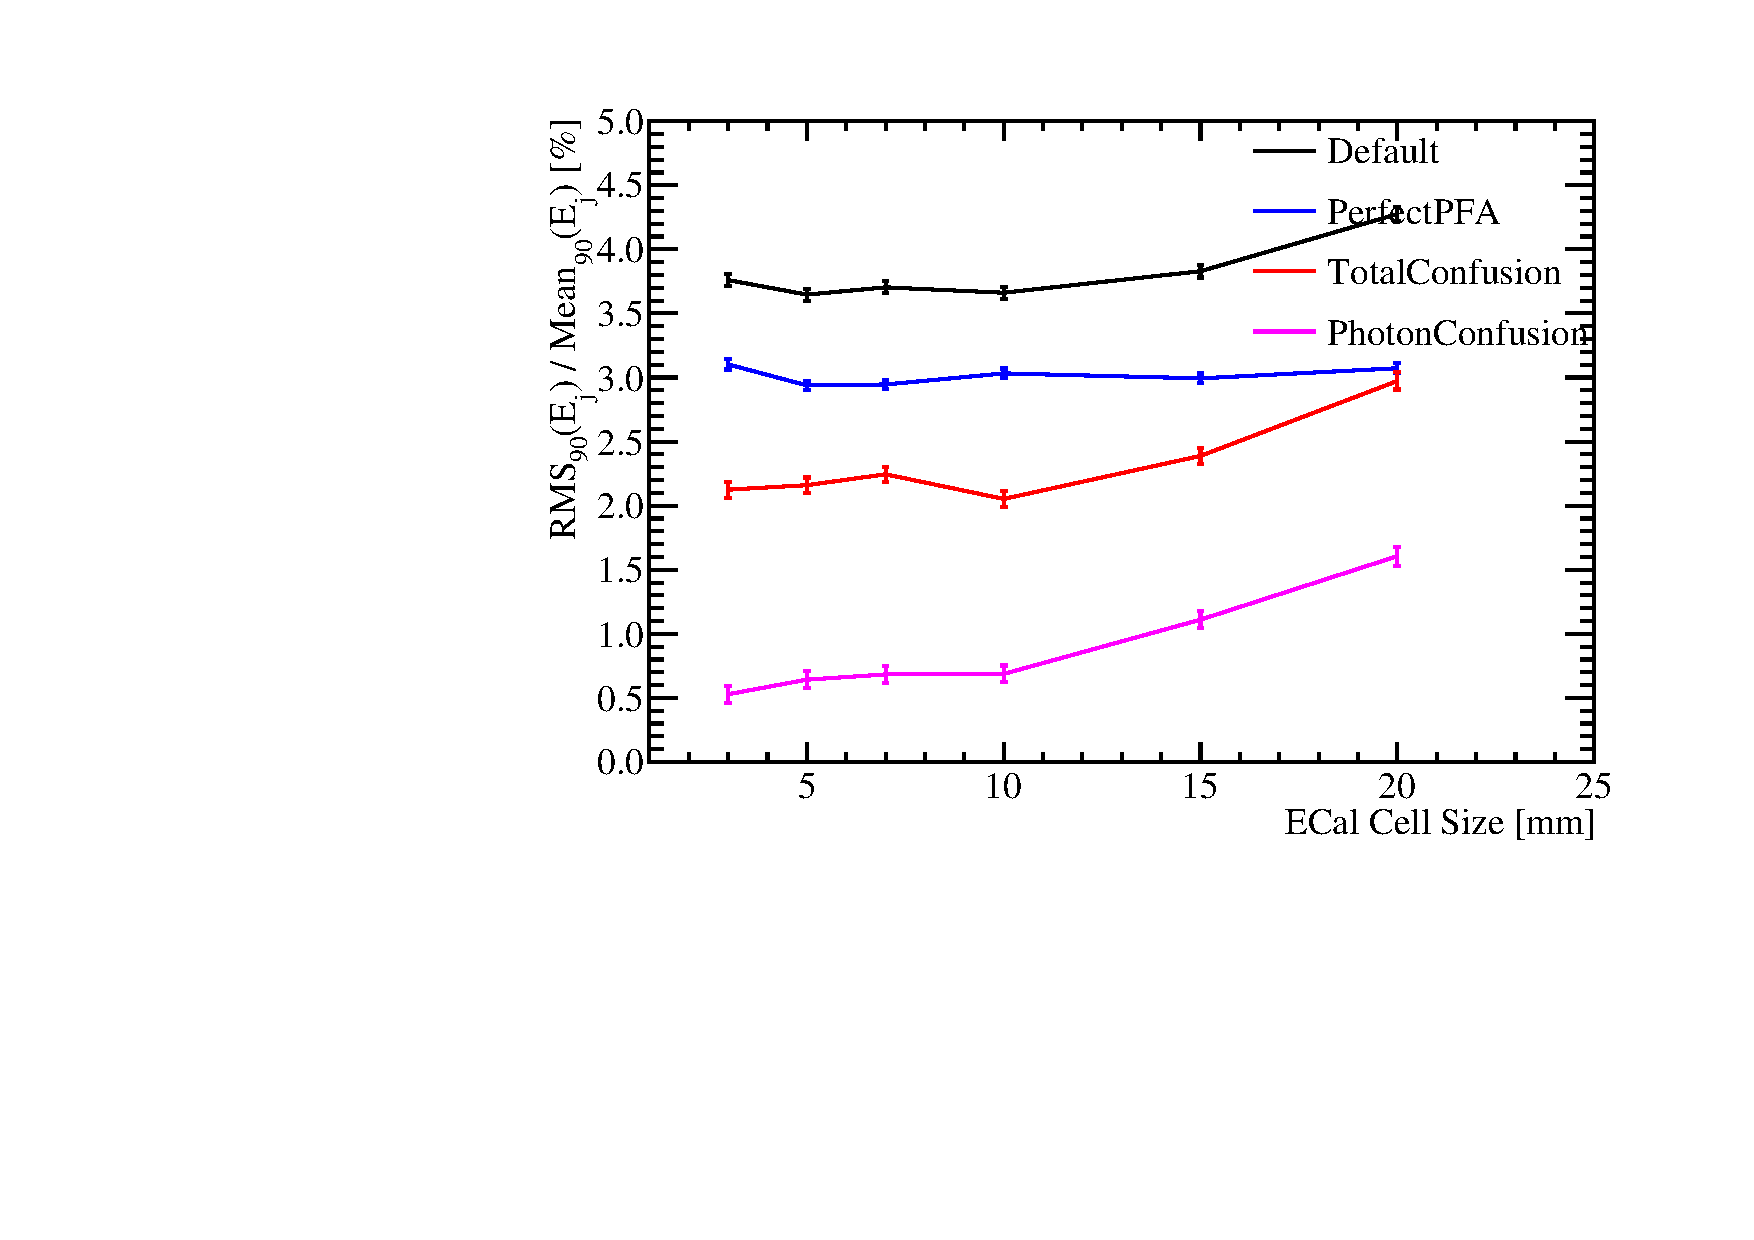
\includegraphics[width=0.5\textwidth]{OptimisationStudies/Plots/JetEnergyResolutions/JER_vs_SiliconECalCellSize_91GeV_DiJet_Breakdown.pdf}}
\subfloat[Scintillator active material, 45 GeV Jets.]{\label{fig:ecalsccellsize45break}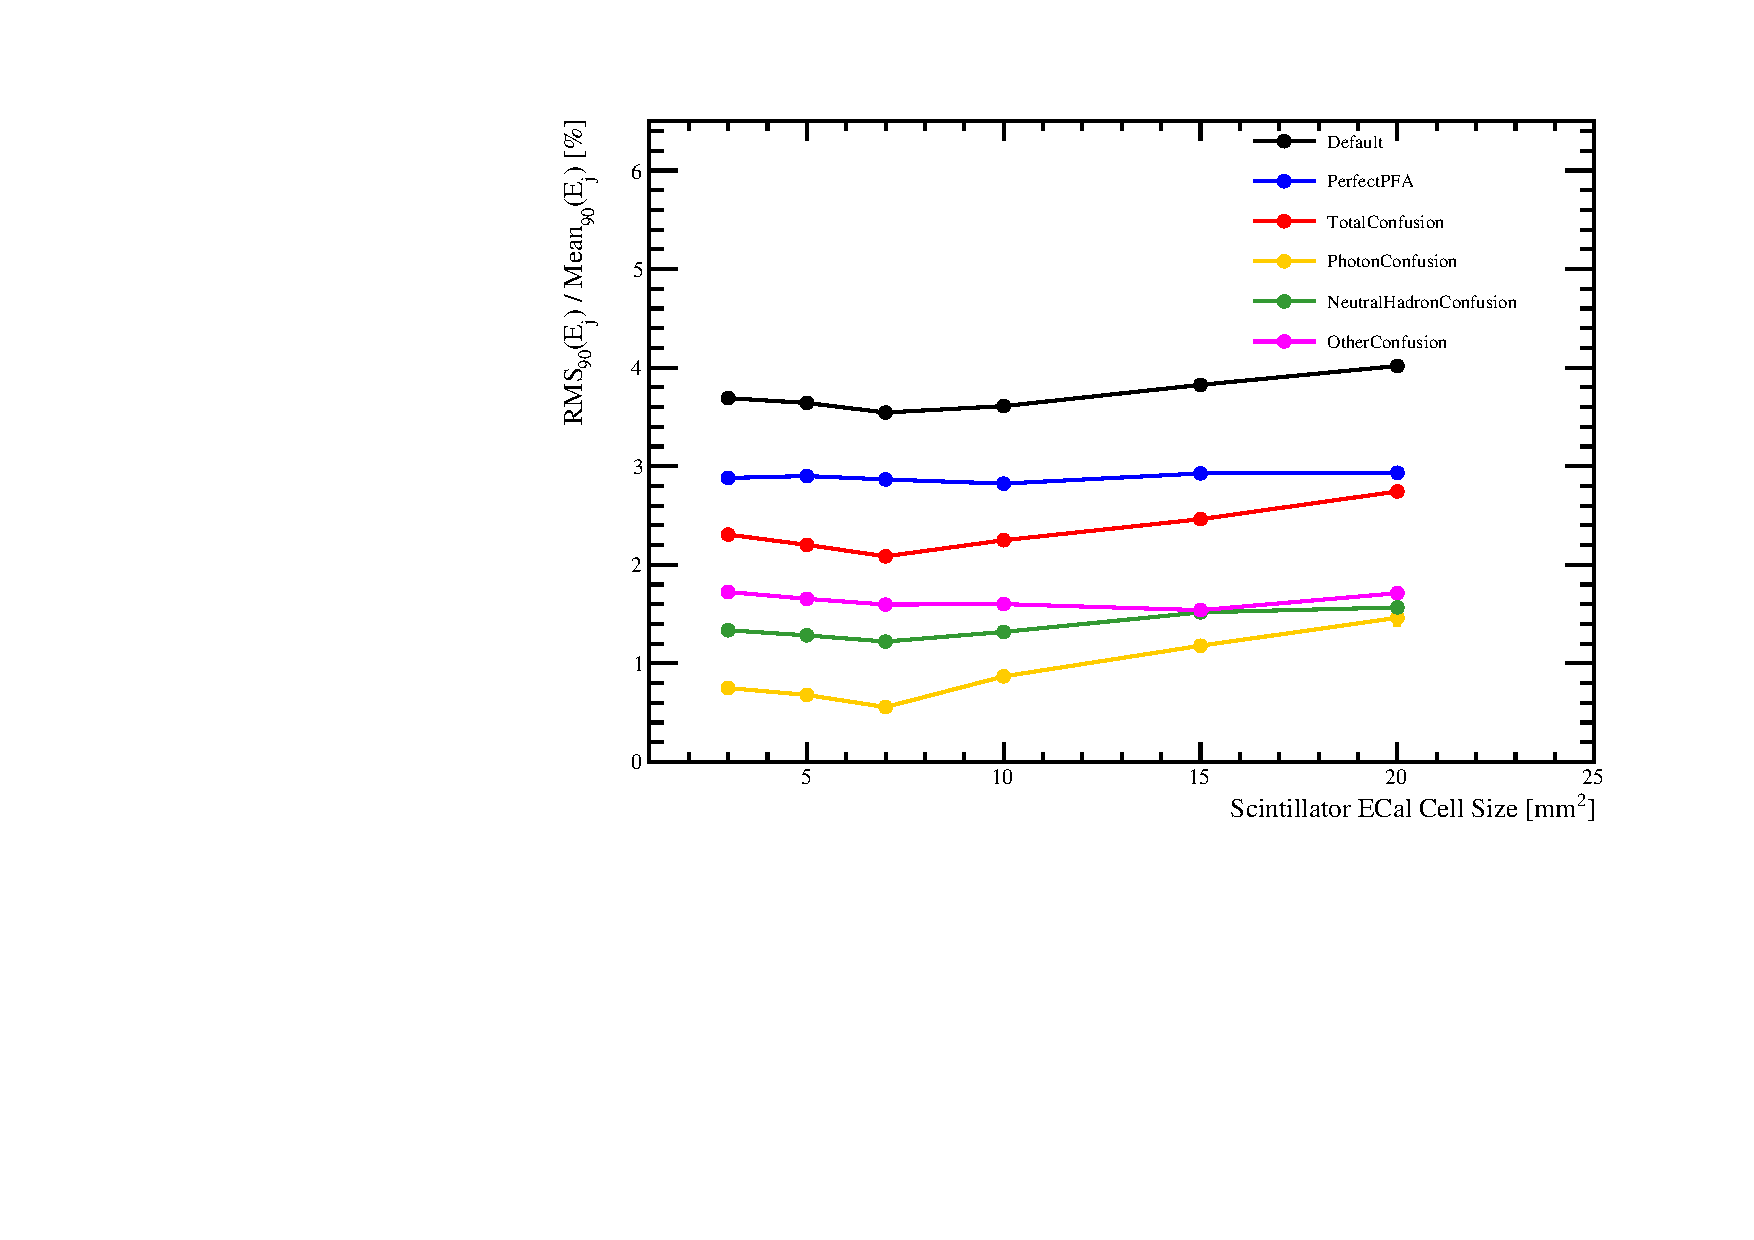
\includegraphics[width=0.5\textwidth]{OptimisationStudies/Plots/JetEnergyResolutions/JER_vs_ScintillatorECalCellSize_91GeV_DiJet_Breakdown.pdf}} \hfill
\subfloat[Silicon active material, 250 GeV Jets.]{\label{fig:ecalsicellsize250break}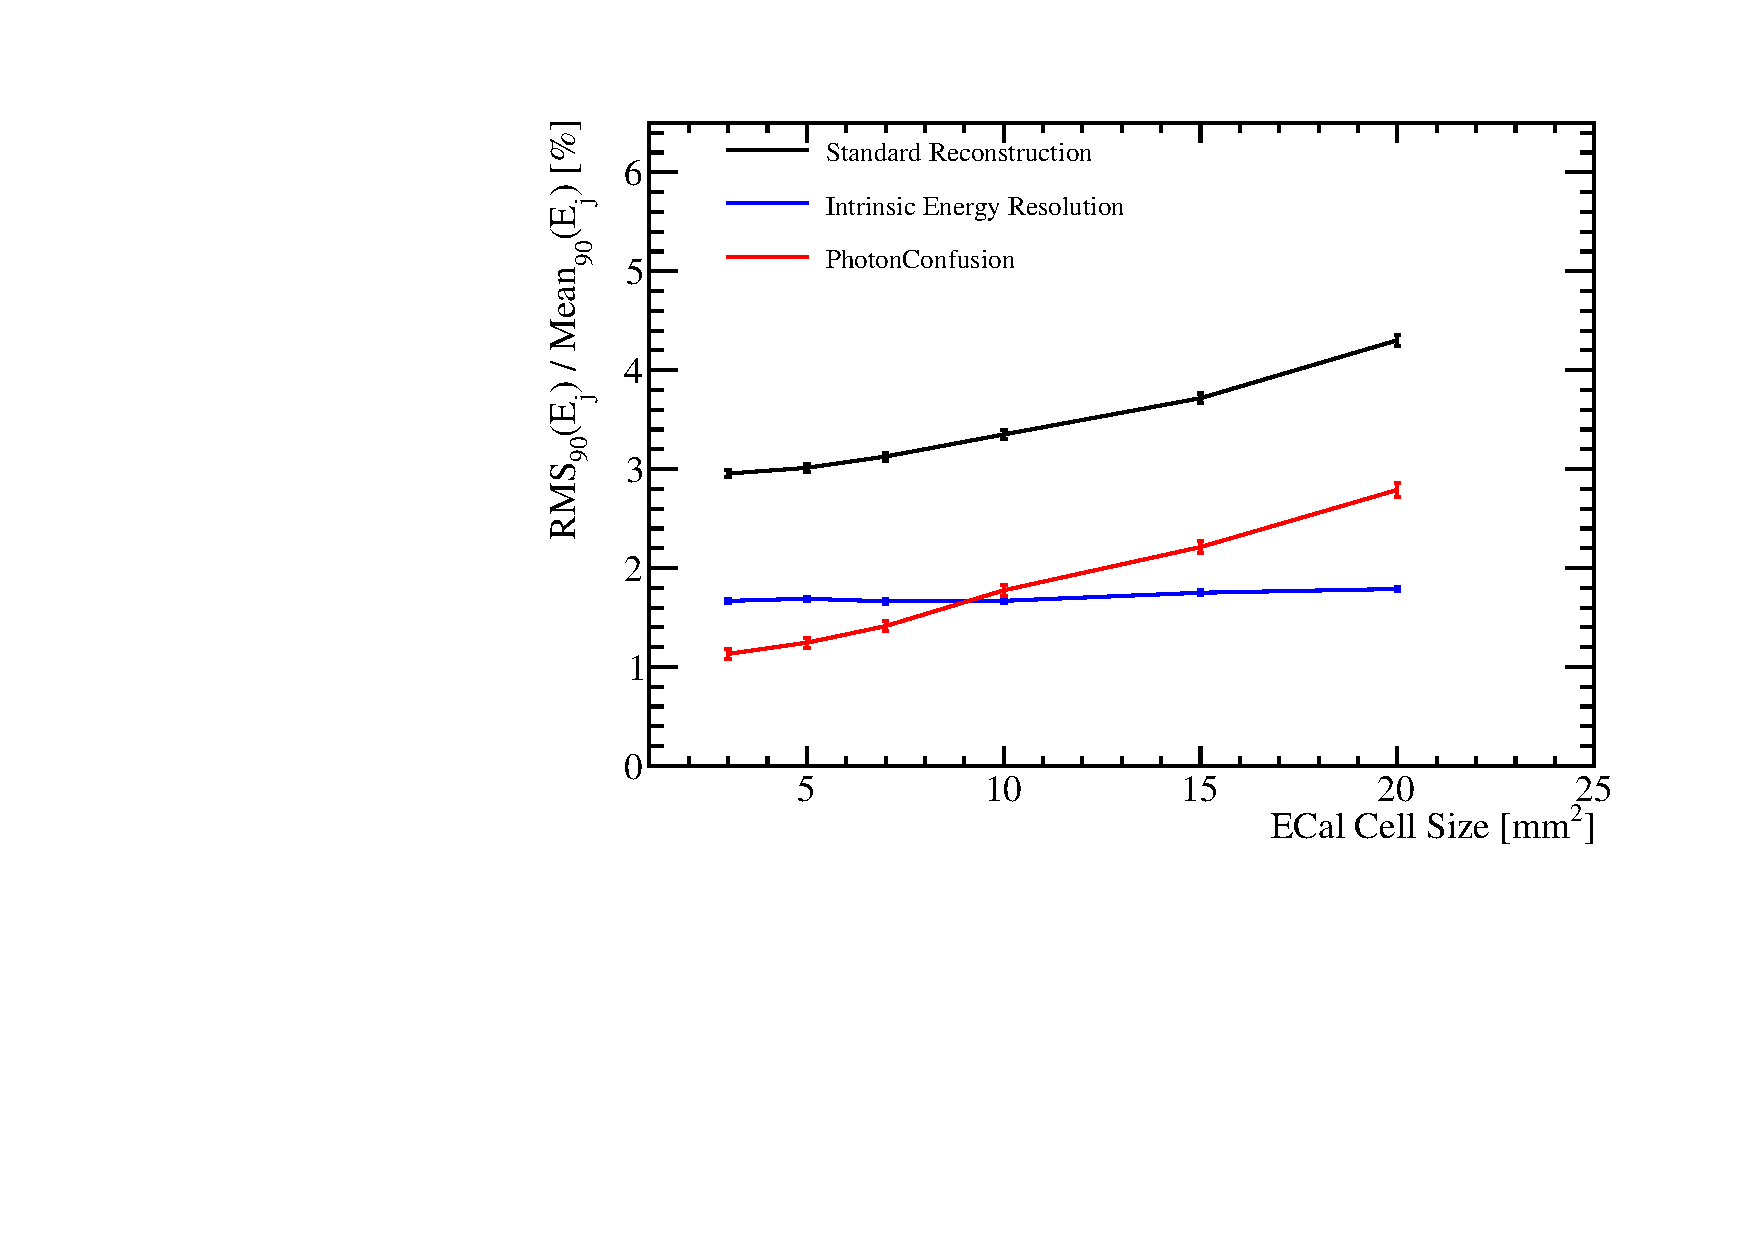
\includegraphics[width=0.5\textwidth]{OptimisationStudies/Plots/JetEnergyResolutions/JER_vs_SiliconECalCellSize_500GeV_DiJet_Breakdown.pdf}}
\subfloat[Scintillator active material, 250 GeV Jets.]{\label{fig:ecalsccellsize250break}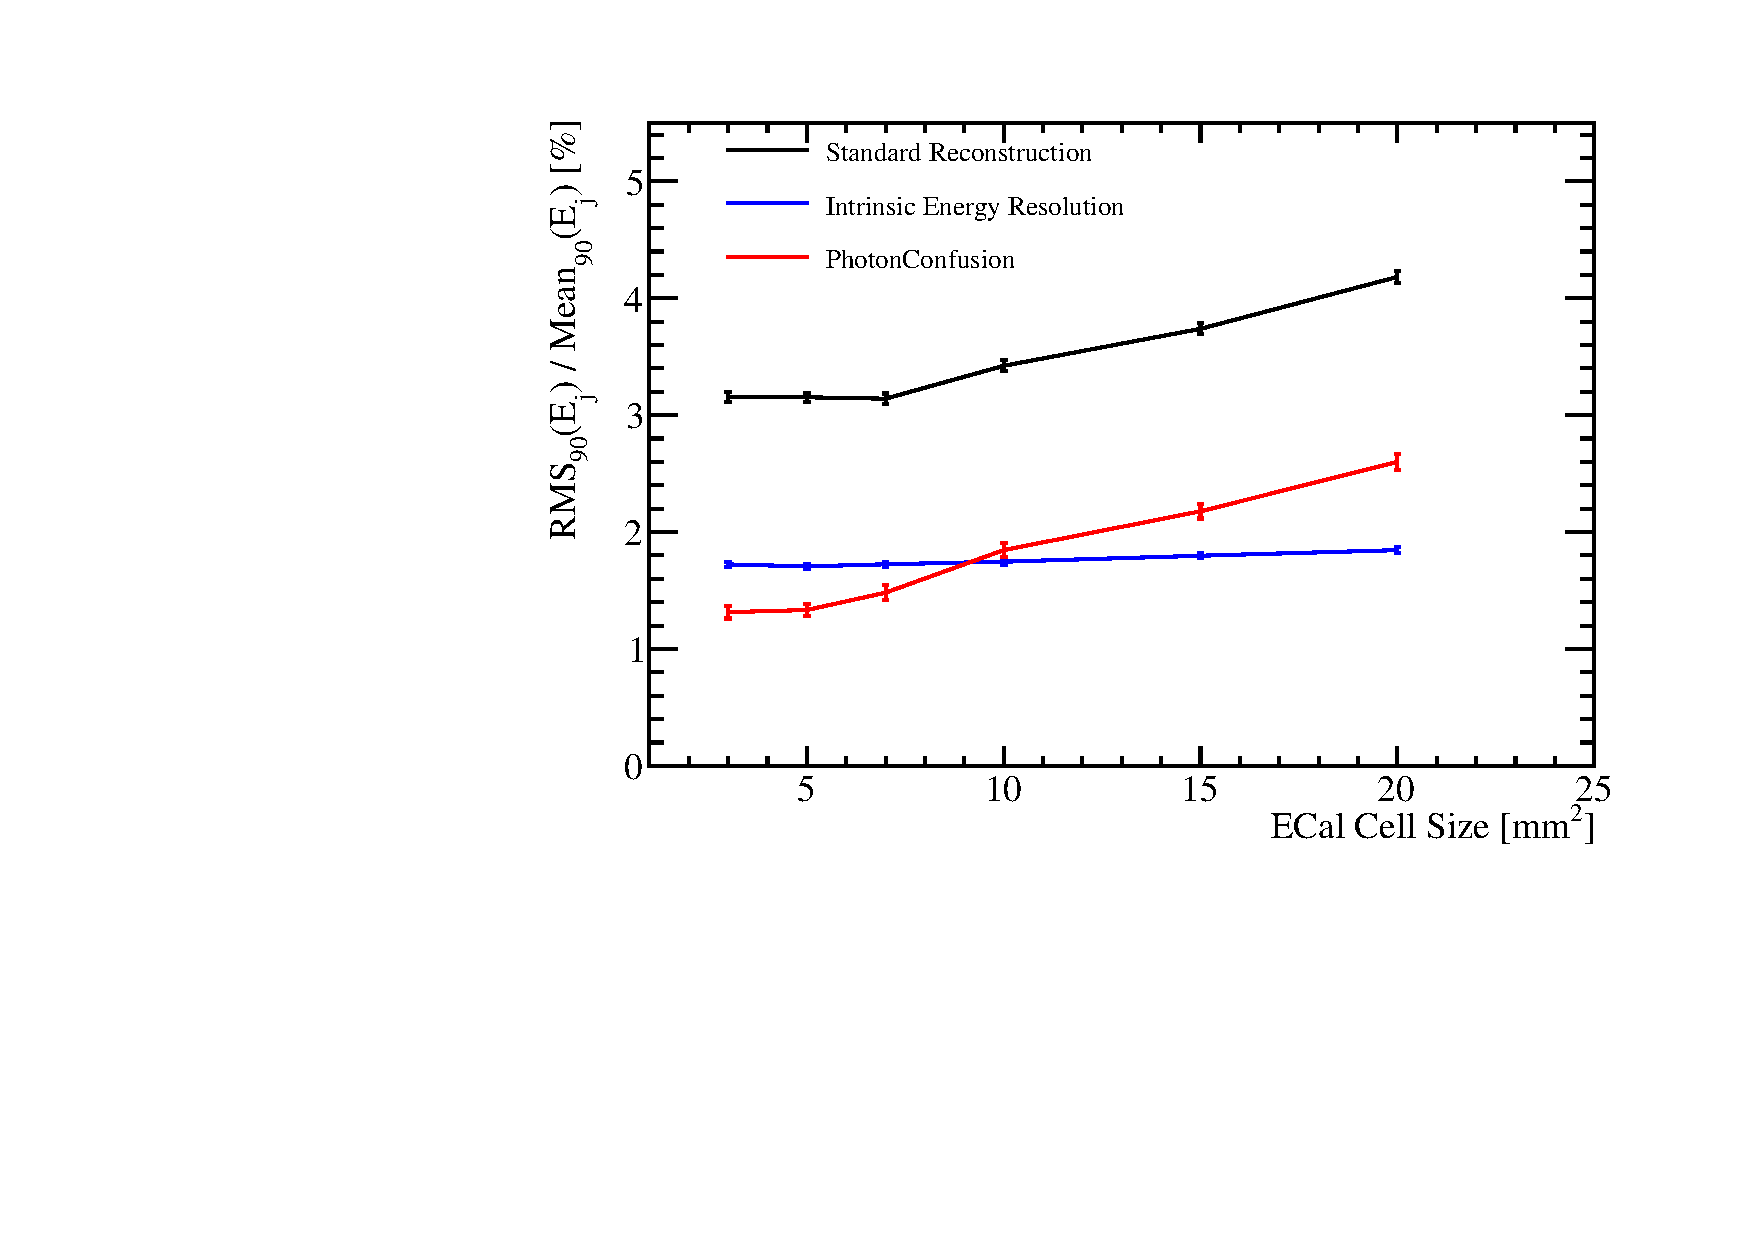
\includegraphics[width=0.5\textwidth]{OptimisationStudies/Plots/JetEnergyResolutions/JER_vs_ScintillatorECalCellSize_500GeV_DiJet_Breakdown.pdf}}
\caption[Jet energy resolution breakdown as a function of ECal transverse granularity for 45 and 250 GeV jets.  Results are given for both the silicon and scintillator ECal options.]{Jet energy resolution breakdown as a function of ECal transverse granularity for 45 and 250 GeV jets.  Results are given for both the silicon and scintillator ECal options.}
\label{fig:ecalcellsizebreak}
\end{figure}

By examining the breakdown of the jet energy resolution into intrinsic resolution and confusion terms, as explained in chapter BLAH, it is possible to conclude that the dominant factor affecting the jet energy resolution when the transverse granularity of the ECal is varied is the confusion arising from photon energy deposits.  Examples of jet energy resolution breakdowns are shown for 45 and 250 GeV jets for both the silicon and scintillator ECal options in figure \ref{fig:ecalcellsizebreak}.  As expected in the intrinsic energy resolution does not change significantly with the transverse granularity.  

\begin{figure}
\centering
%\subfloat[Silicon active material, 10 GeV $\gamma$.]{\label{fig:ecalsicellsize10gamma}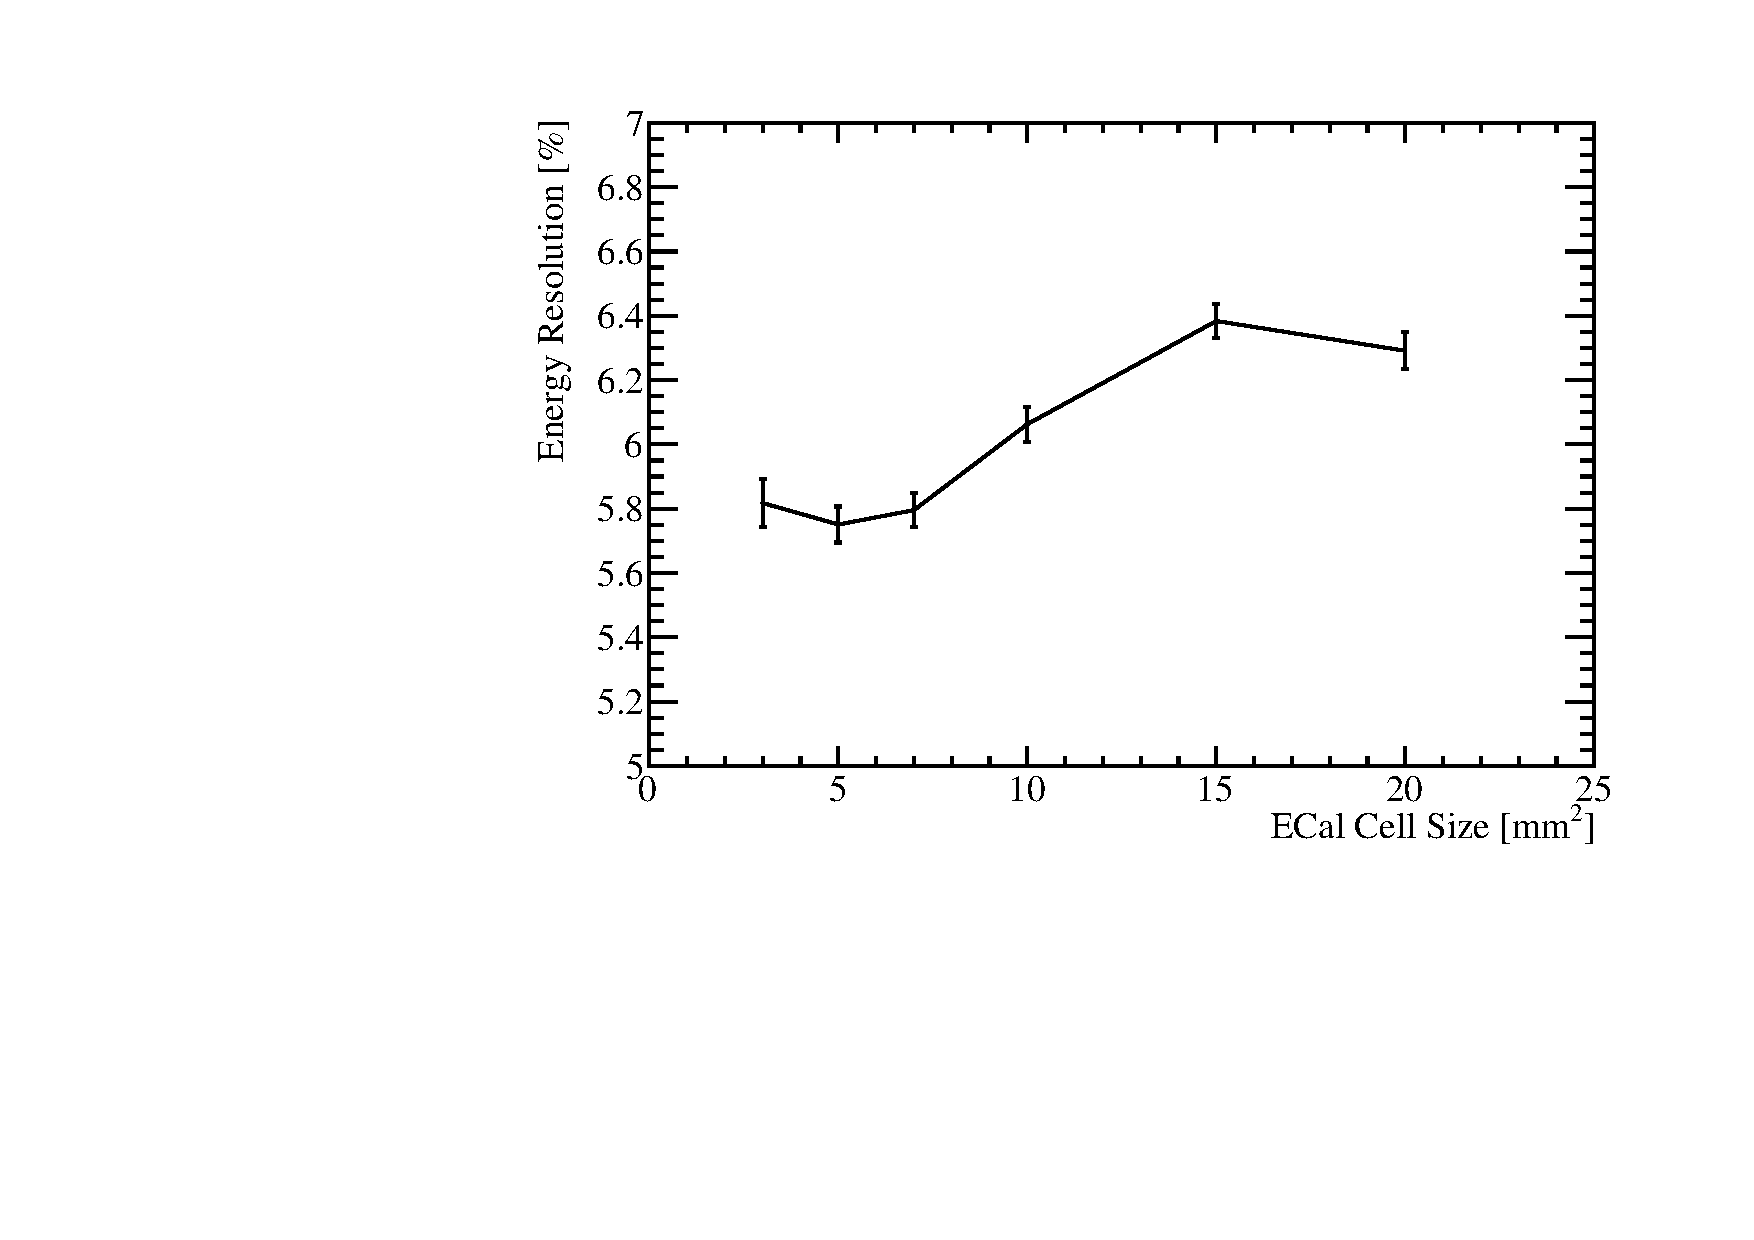
\includegraphics[width=0.5\textwidth]{OptimisationStudies/Plots/EnergyResolution/SiECal10GeVPhotonResVsCellSize.pdf}} // Bit too messy to draw good conclusions
%\subfloat[Scintillator active material, 10 GeV $\gamma$.]{\label{fig:ecalsccellsize10gamma}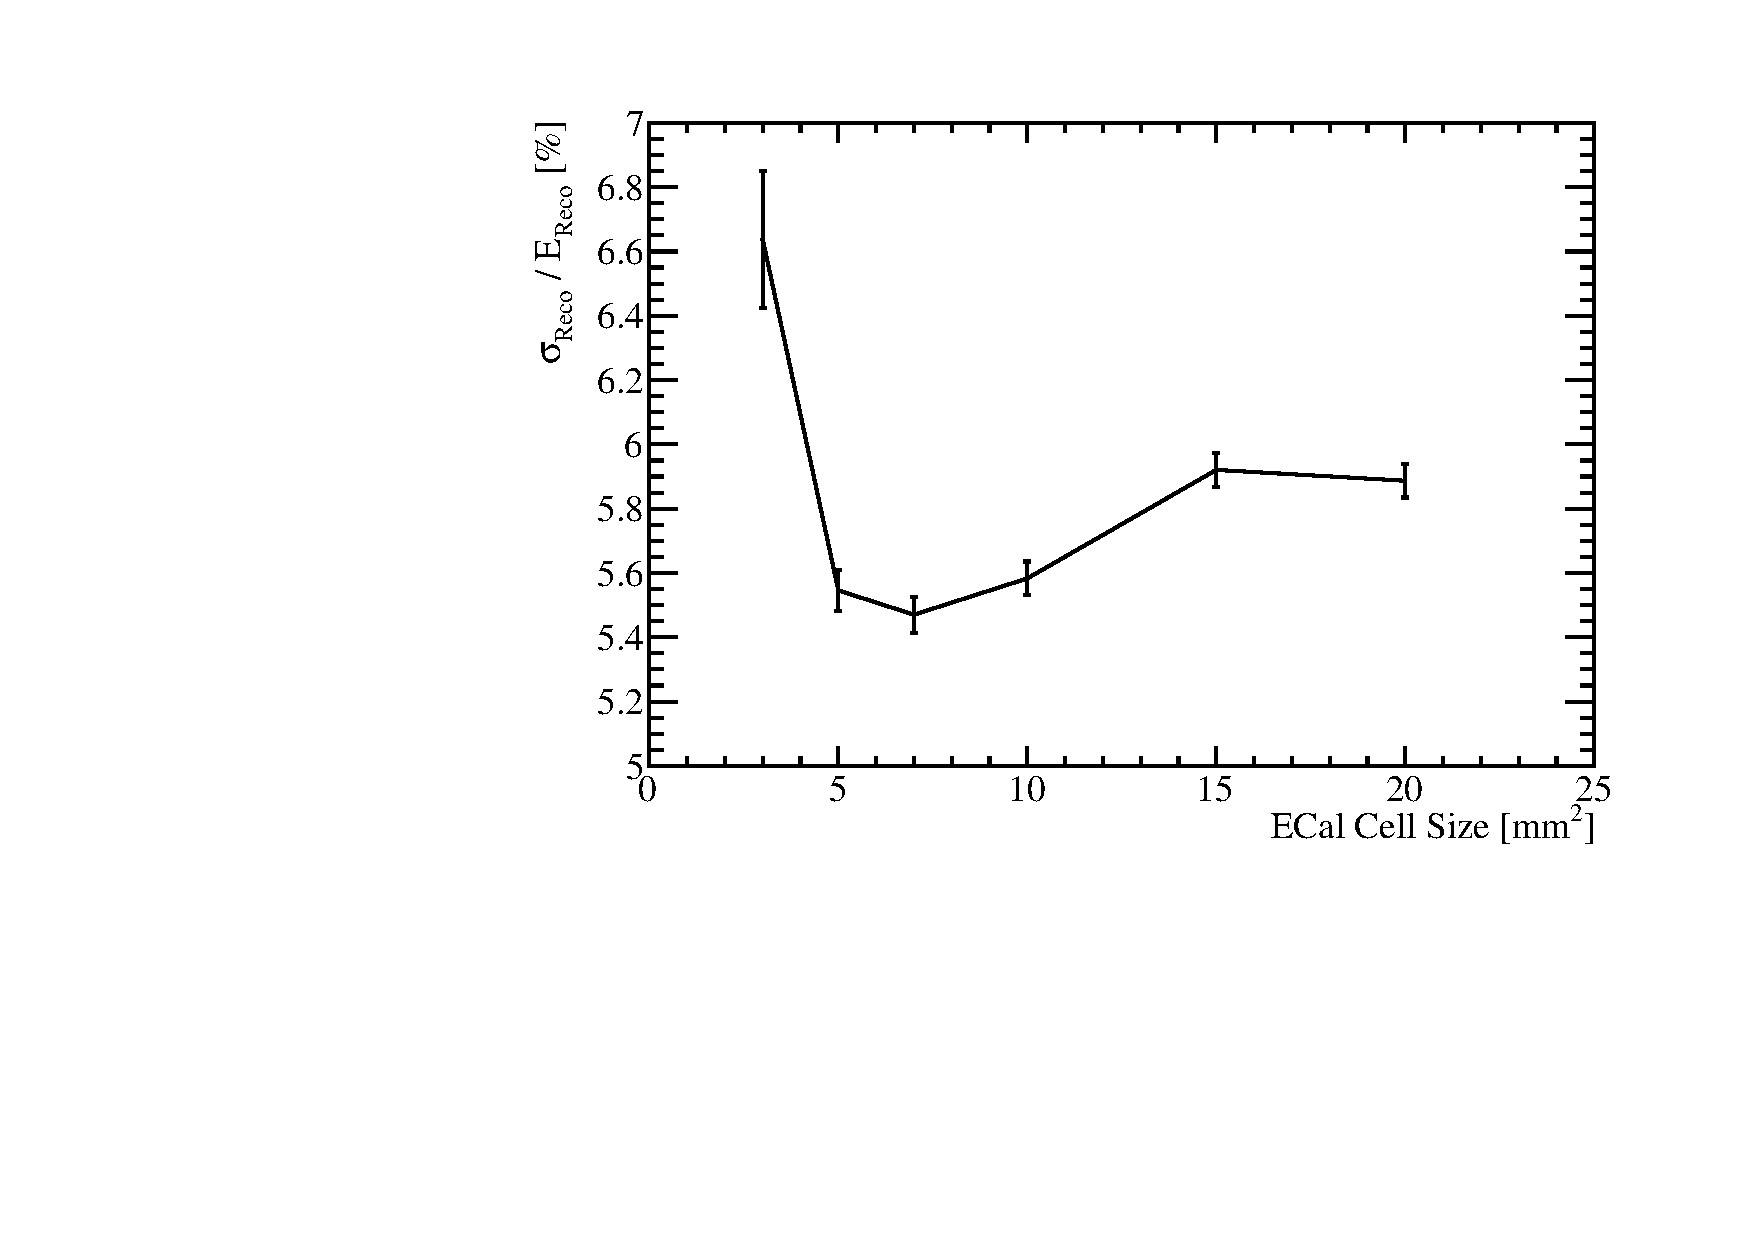
\includegraphics[width=0.5\textwidth]{OptimisationStudies/Plots/EnergyResolution/ScECal10GeVPhotonResVsCellSize.pdf}} \hfil // Bit too messy to draw good conclusions
\subfloat[Silicon active material, 100 GeV $\gamma$.]{\label{fig:ecalsicellsize100gamma}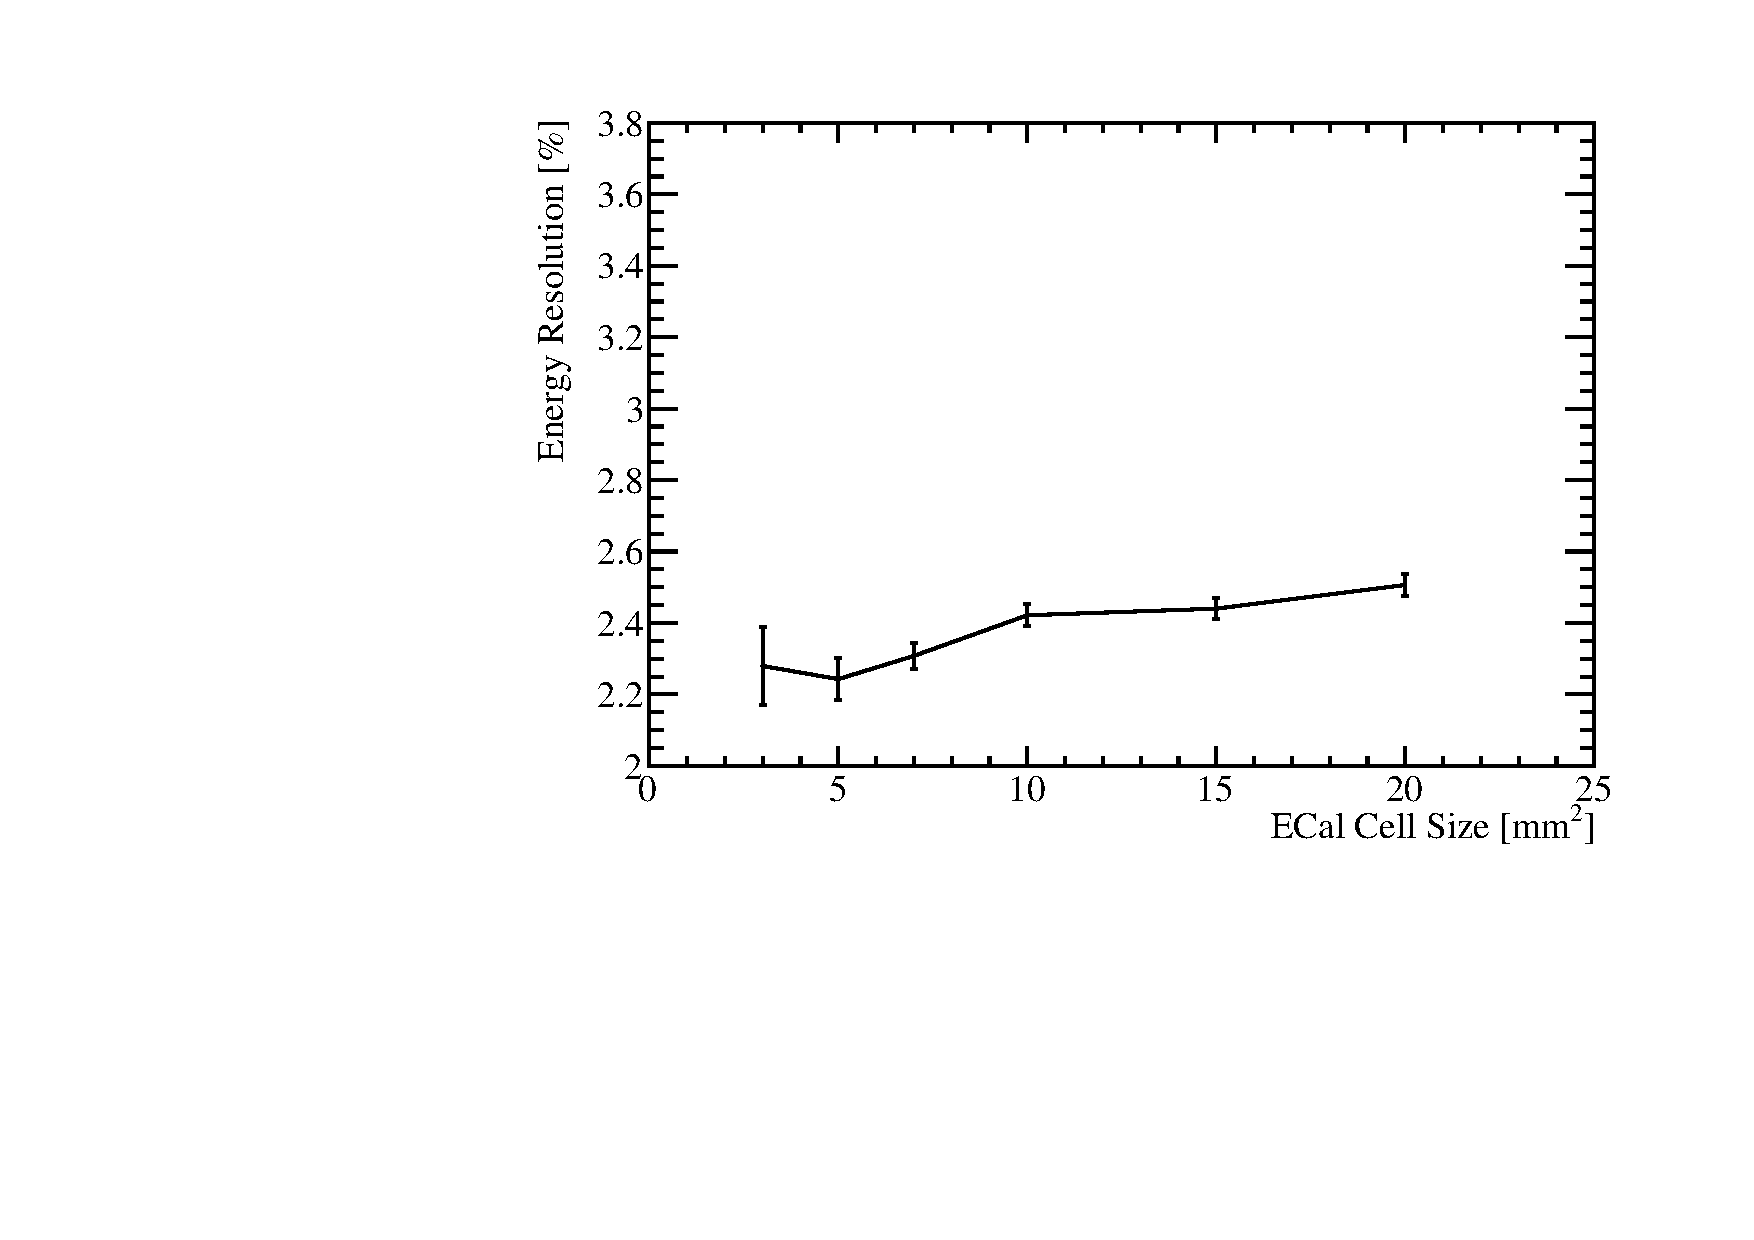
\includegraphics[width=0.5\textwidth]{OptimisationStudies/Plots/EnergyResolution/SiECal100GeVPhotonResVsCellSize.pdf}}
\subfloat[Scintillator active material, 100 GeV $\gamma$.]{\label{fig:ecalsccellsize100gamma}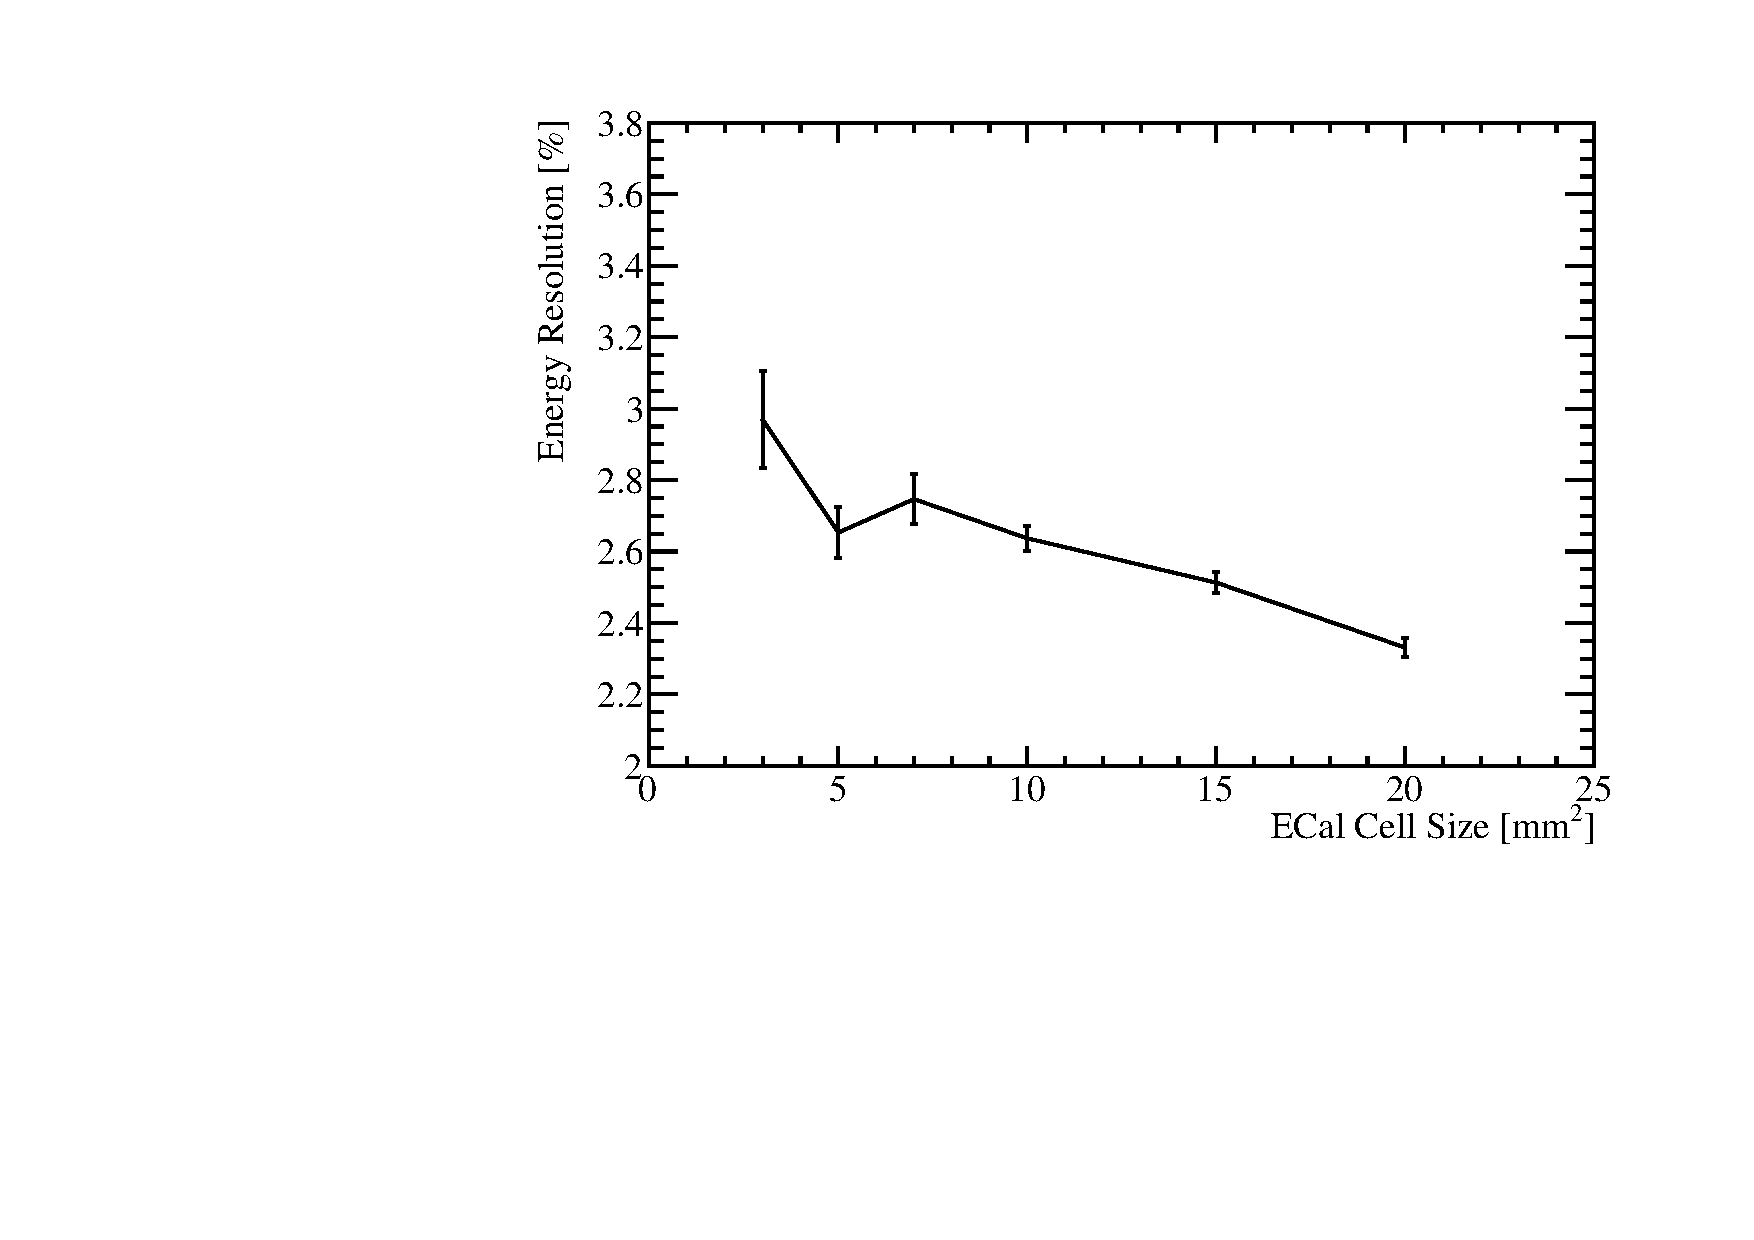
\includegraphics[width=0.5\textwidth]{OptimisationStudies/Plots/EnergyResolution/ScECal100GeVPhotonResVsCellSize.pdf}}
\caption[Energy resolution as a function of ECal transverse granularity for 100 GeV photons.  Results are given for both the silicon and scintillator ECal options.]{Energy resolution as a function of ECal transverse granularity for 100 GeV photons.  Results are given for both the silicon and scintillator ECal options.}
\label{fig:ecalcellsizegamma}
\end{figure}

A more targeted test of the intrinsic energy resolution of the ECal is presented in figure \ref{fig:ecalcellsizegamma}, which examines the energy resolution of single photon samples at 100 GeV.  For the silicon option the intrinsic energy resolution was found to not vary significantly across the transverse granularities under consideration, however, there is a degradation in energy resolution with increasing cell size for the scintillator option.  This originates from an inactive region of material in the simulation that represents the multi pixel photon counter (MPPC).  The MPPC occupies a fixed area of the cell irrespective of cell size and so fractionally the "dead" region of the cell increases as cell size is reduced (cite this somehow).  These trends will be present in the jet energy resolution studies, however, as only a small fraction, $\approx 10$\%, of the jet energy arises from the ECal these trends will be washed out when looking purely at jets.

In conclusion smaller transverse granularities in the ECal significantly improve the jet energy resolution for both the silicon and scintillator options.  The intrinsic energy resolution of the ECal is largely invariant to changes in the transverse granularity for the silicon option, while larger transverse granularities are beneficial to the scintillator option as they reduce the impact of "dead" regions of the detector.  

%========================================================================================

\subsection{ECal Longitudinal Granularity}
\label{sec:ecalnlayers}
The performance of a number of detector configurations was examined where the longitudinal granularity of the ECal absorber material had been varied about the nominal value.  This study was performed for both the silicon and scintillator active material options.  In all cases considered tungsten was used as the absorber material in the ECal and the active layer thicknesses were not changed, that is 0.5 mm for the silicon option and 2 mm for the scintillator option.  The layout of the ECal for detector models considered are summarised in table \ref{table:nlayersecaloption}.  For each detector model considered in this study the total number of radiation lengths in the ECal is kept approximately constant.  This is done by varying the thickness of the absorber material when modifying the number of layers in the ECal. 

 \begin{table}[h!]
\centering
\begin{tabular}{ l l l l l l}
\hline
Total Number & $N_{Layers}$ & Absorber & $N_{Layers}$ & Absorber & Total  \\
of Layers & Region 1 & Thickness & Region 2 & Thickness & Thickness \\
$N_{\text{Layers ECal}}$ & & Region 1 [mm] & &  Region 2 [mm] &  [$\text{X}_{0}$] \\

\hline
30 & 20 & 2.10 & 9 & 4.20 & 22.77 \\
26 & 17 & 2.40 & 8 & 4.80 & 22.60 \\
20 & 13 & 3.15 & 6 & 6.30 & 22.47 \\
16 & 10 & 4.00 & 5 & 8.00 & 22.31\\
\hline
\end{tabular}
\caption[Transverse granularity layout of various ECal models considered in this study.]{Transverse granularity layout of various ECal models considered in this study.  Radiation length of tungsten absorber is 3.504mm \cite{Olive:2016xmw}.  Note that the presampler layer contributes one layer to the cumulative number of layers value for all detector models considered.}
\label{table:nlayersecaloption}
\end{table}

\begin{figure}
\centering
\subfloat[Silicon active material.]{\label{fig:ecalsinlayers}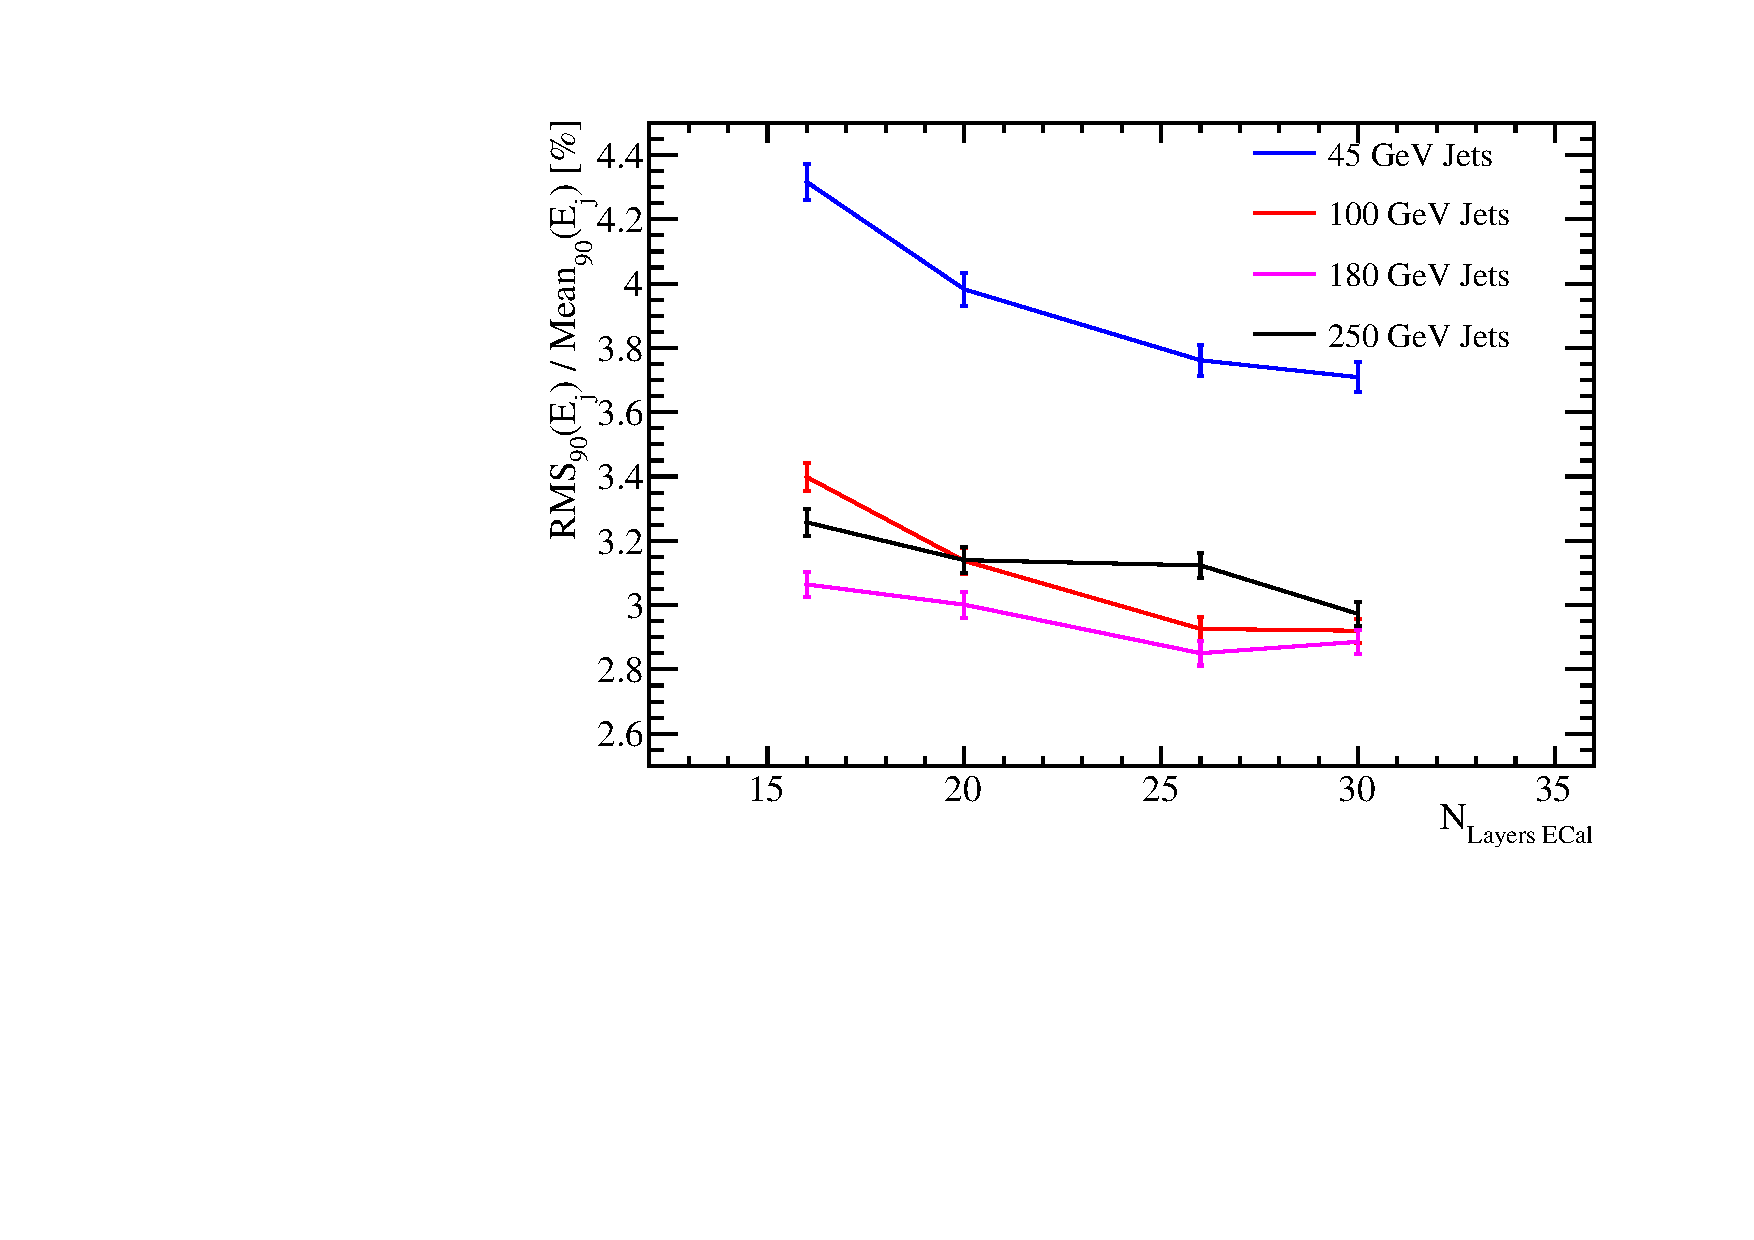
\includegraphics[width=0.5\textwidth]{OptimisationStudies/Plots/JetEnergyResolutions/JER_vs_SiliconECalNumberofLayers.pdf}}
\subfloat[Scintillator active material.]{\label{fig:ecalscnlayers}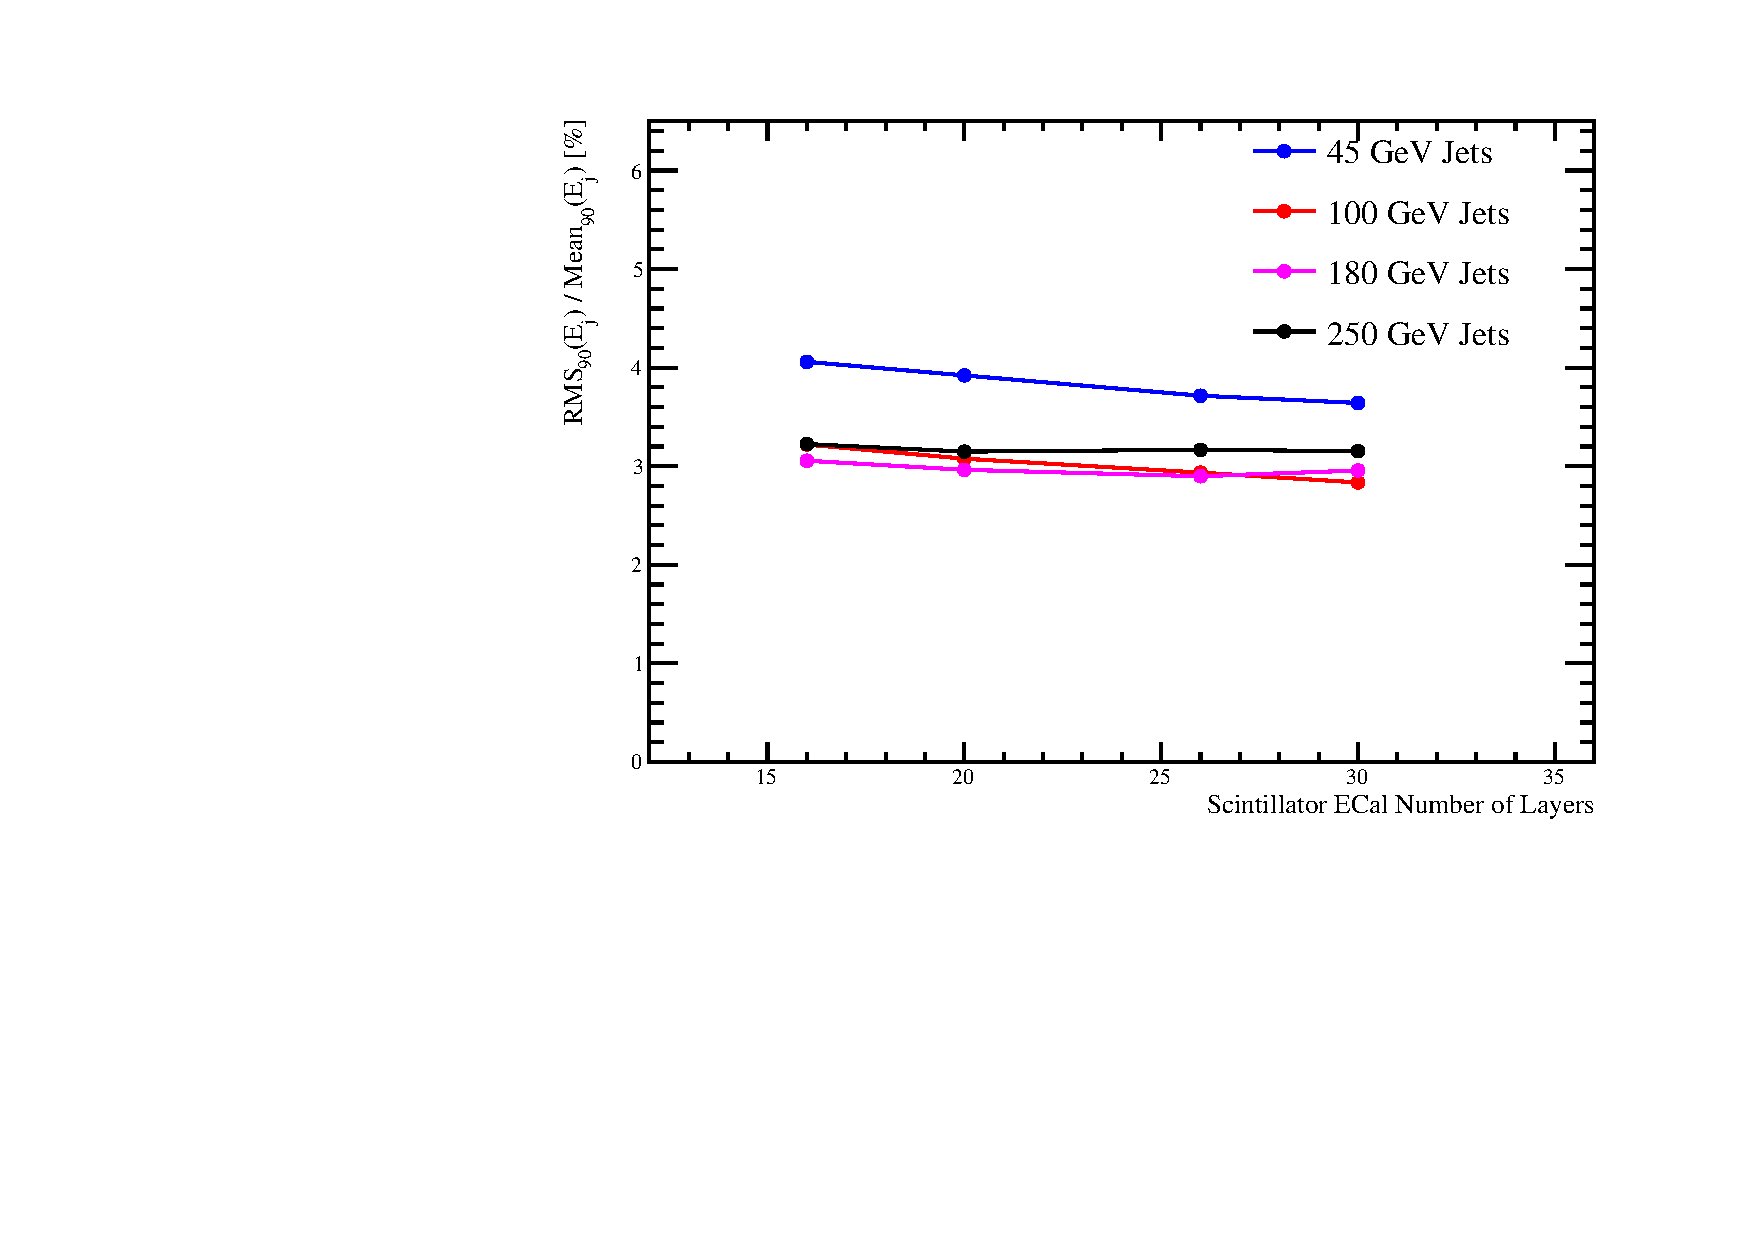
\includegraphics[width=0.5\textwidth]{OptimisationStudies/Plots/JetEnergyResolutions/JER_vs_ScintillatorECalNumberofLayers.pdf}} \hfill
\caption[Jet energy resolution as a function of longitudinal granularity in the ECal.]{Jet energy resolution as a function of longitudinal granularity in the ECal for the silicon and scintillator ECal options.}
\label{fig:ecalnlayers}
\end{figure}

The jet energy resolution was found to improve with increasing longitudinal granularity.  This is expected as a more layers in the calorimeter, for the same total thickness, implies greater sampling of the particle shower and so, as the energy resolution obeys Poissonian statistics, an improvement in the intrinsic energy resolution is observed.  A particularly strong dependancy on ECal longitudinal granularity is noted at low energies, but this reduces significantly as energies rise. 

\begin{figure}
\centering
\subfloat[Silicon active material, 45 GeV Jets.]{\label{fig:ecalsinlayers45break}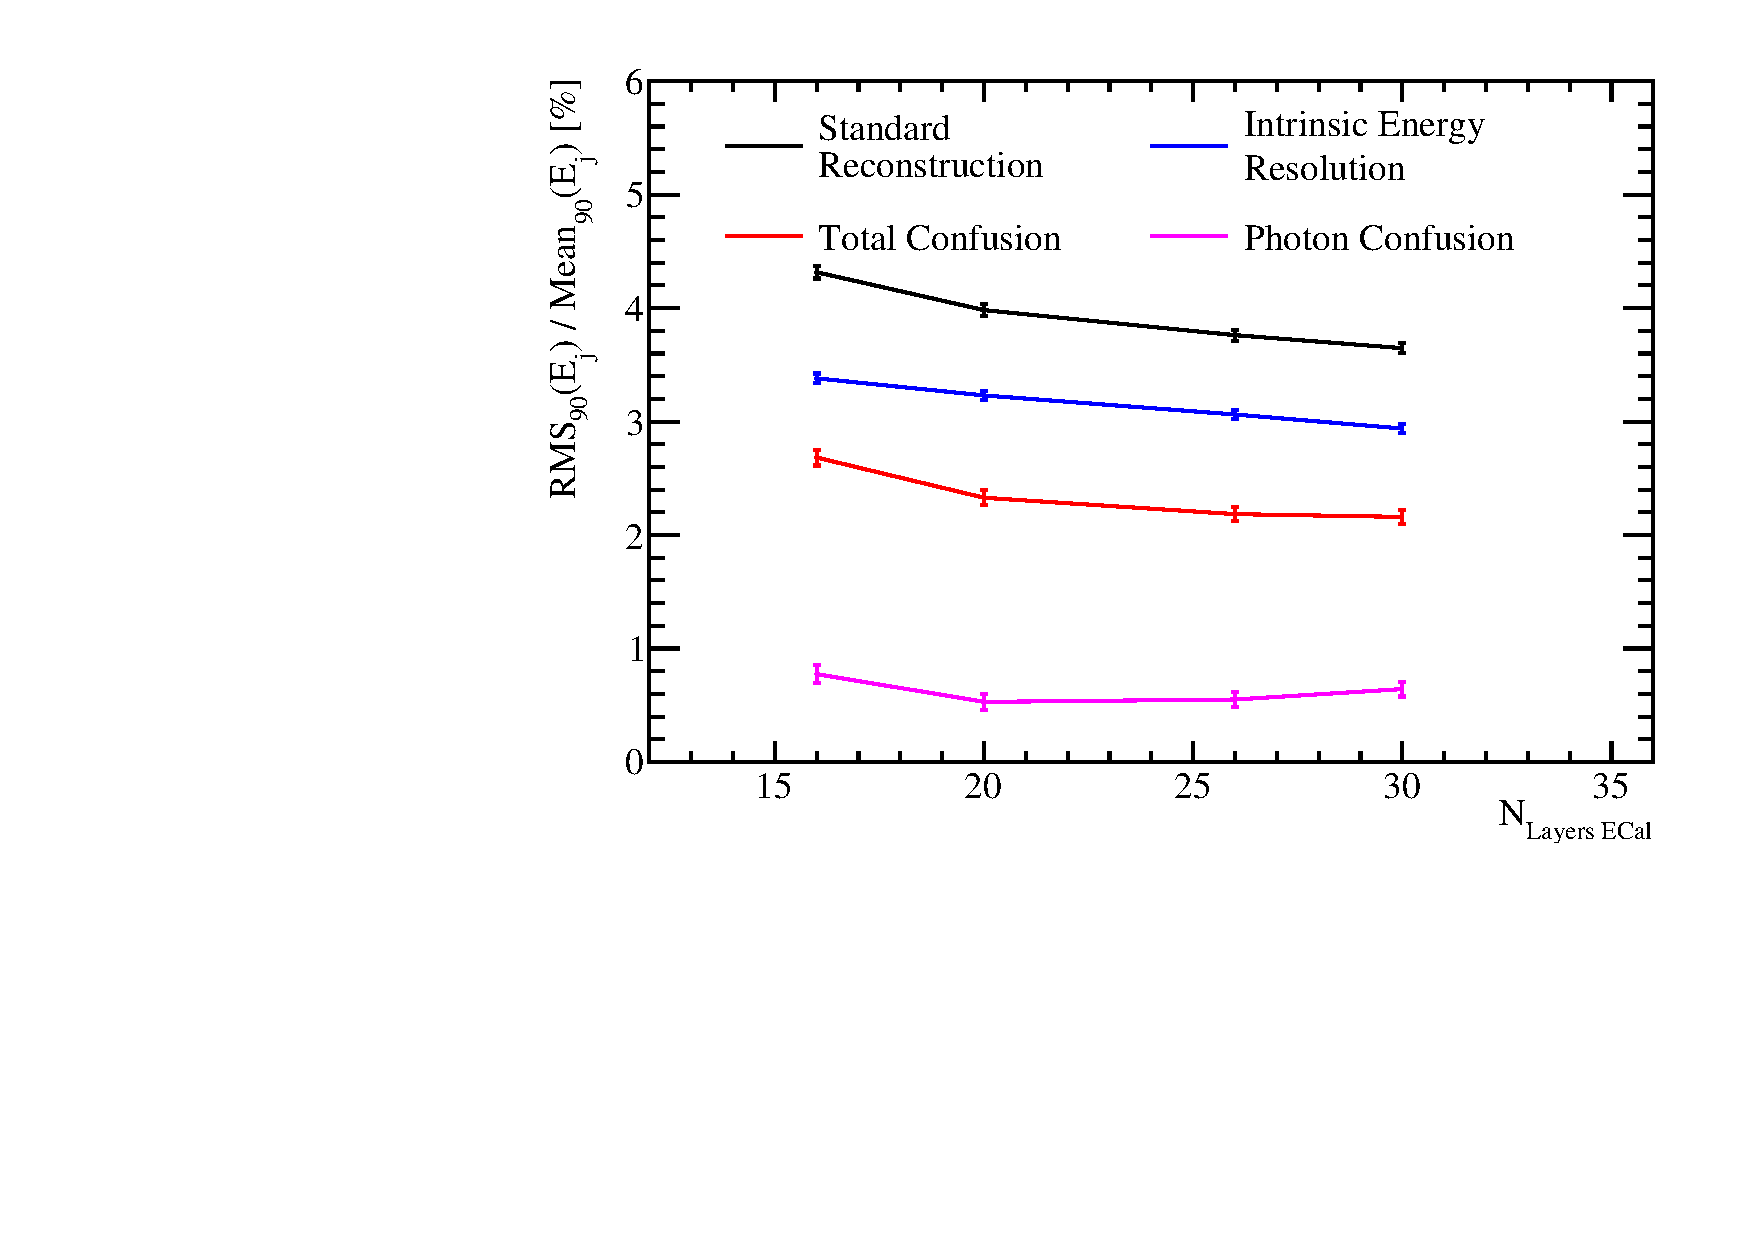
\includegraphics[width=0.5\textwidth]{OptimisationStudies/Plots/JetEnergyResolutions/JER_vs_SiliconECalNumberofLayers_91GeV_DiJet_Breakdown.pdf}}
\subfloat[Scintillator active material, 45 GeV Jets.]{\label{fig:ecalscnlayers45break}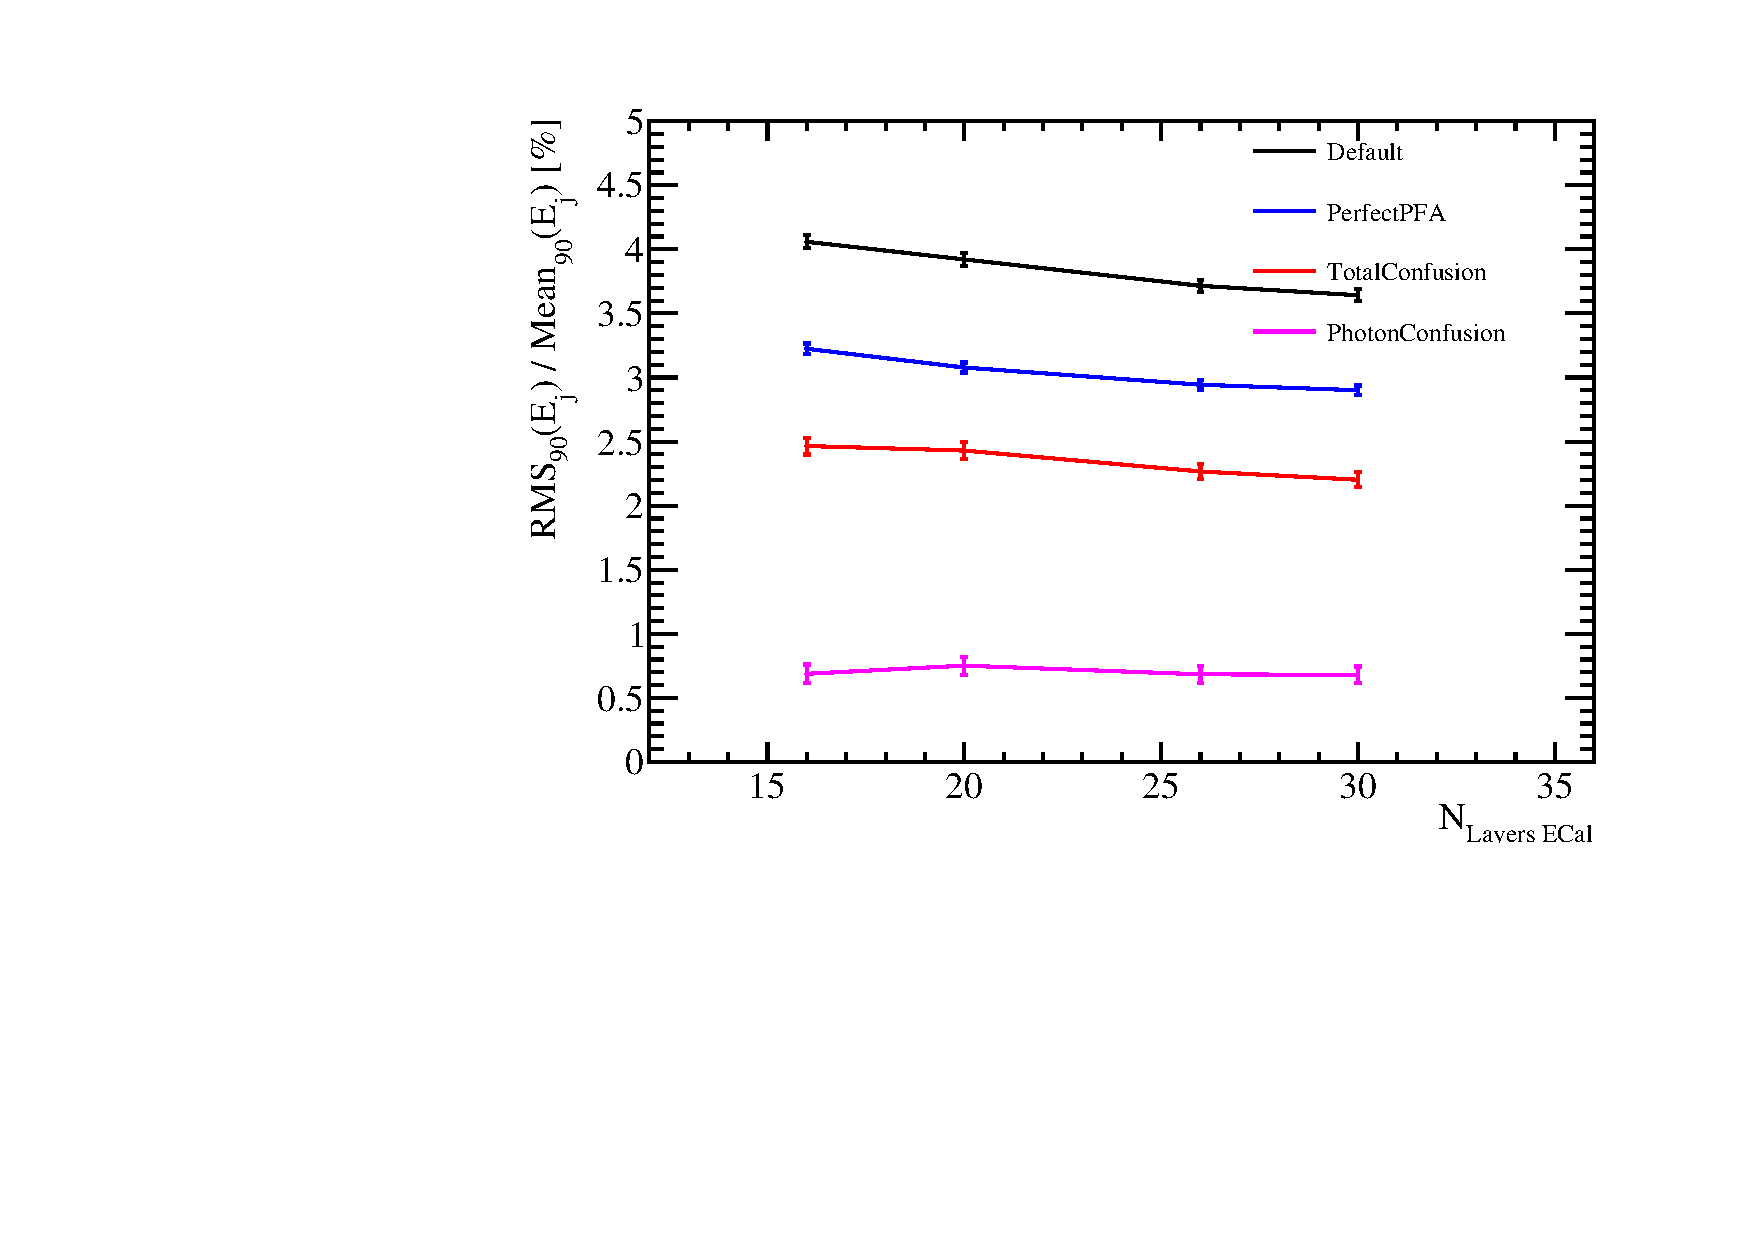
\includegraphics[width=0.5\textwidth]{OptimisationStudies/Plots/JetEnergyResolutions/JER_vs_ScintillatorECalNumberofLayers_91GeV_DiJet_Breakdown.pdf}} \hfill
\subfloat[Silicon active material, 250 GeV Jets.]{\label{fig:ecalsinlayers250break}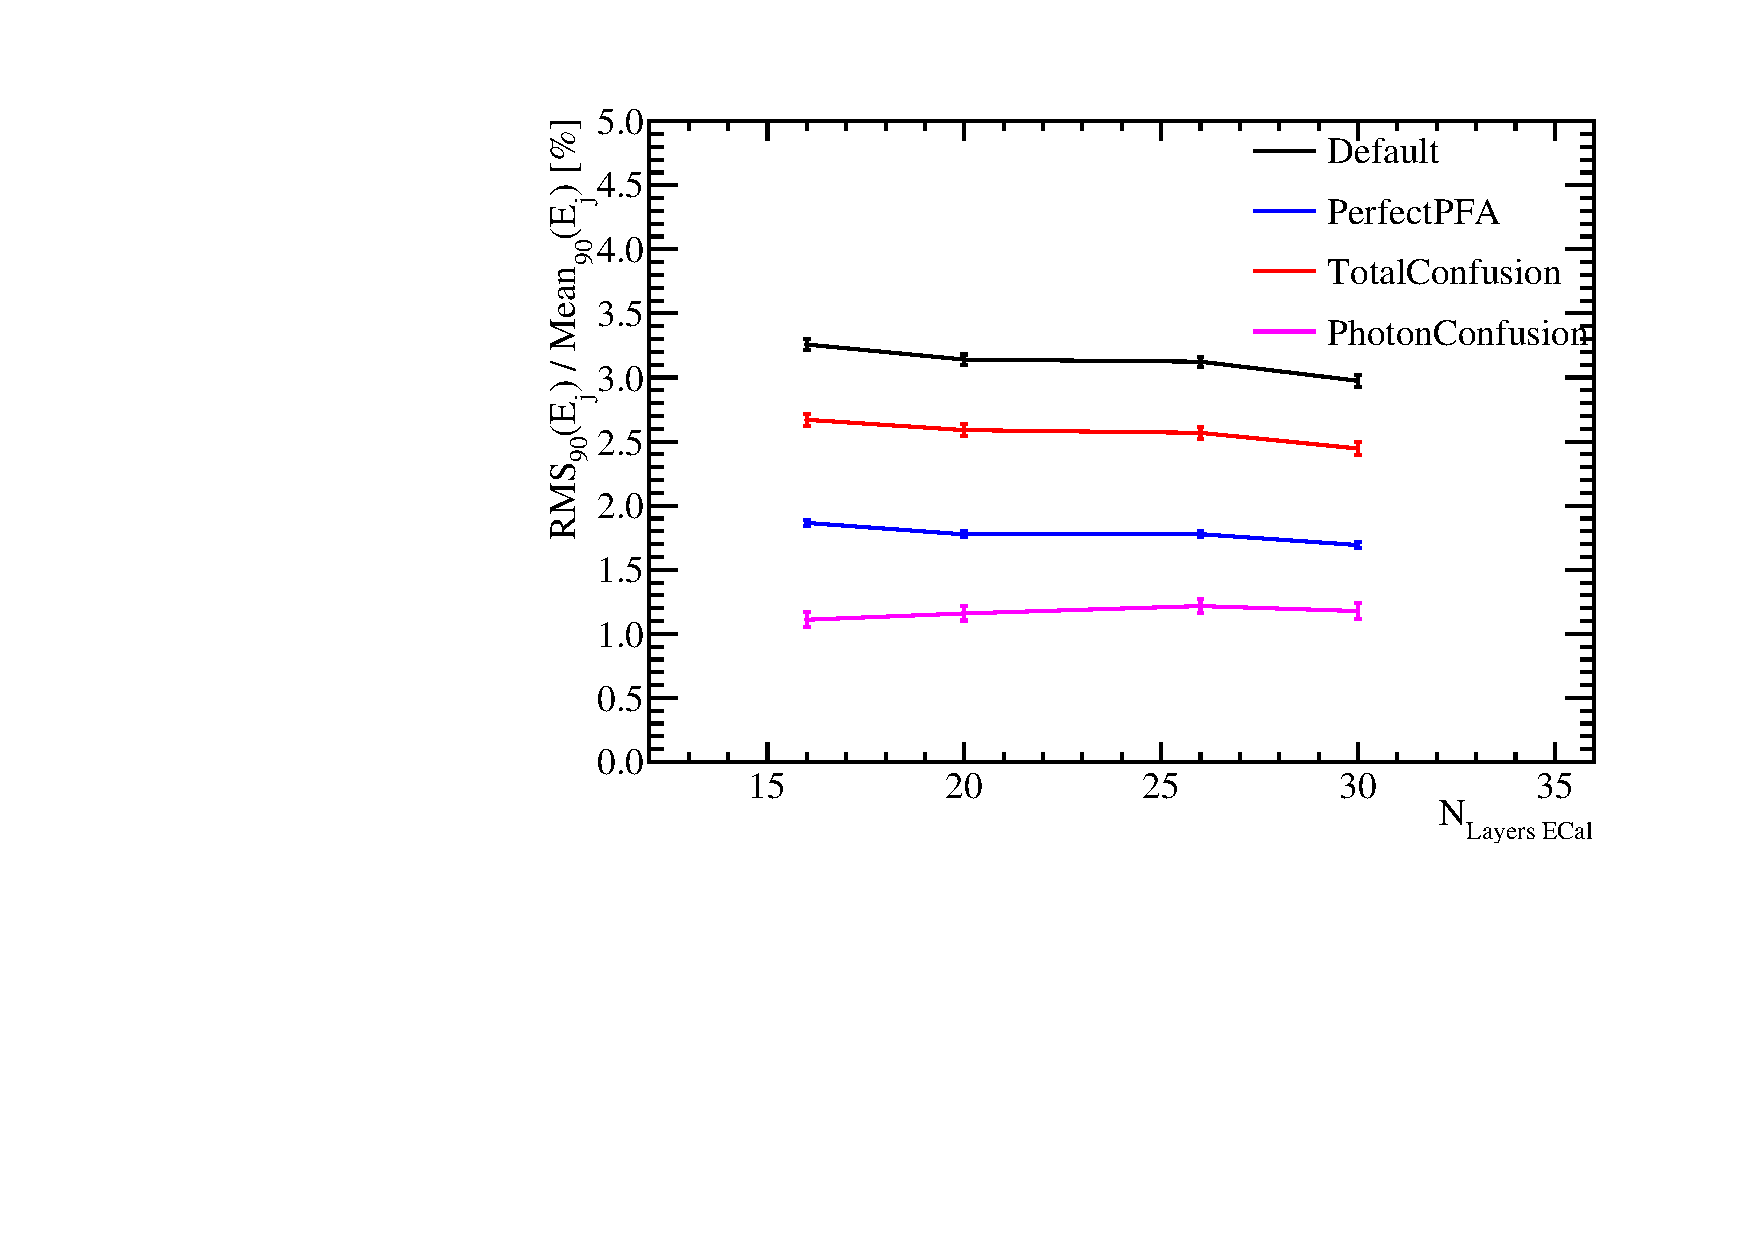
\includegraphics[width=0.5\textwidth]{OptimisationStudies/Plots/JetEnergyResolutions/JER_vs_SiliconECalNumberofLayers_500GeV_DiJet_Breakdown.pdf}}
\subfloat[Scintillator active material, 250 GeV Jets.]{\label{fig:ecalscnlayers250break}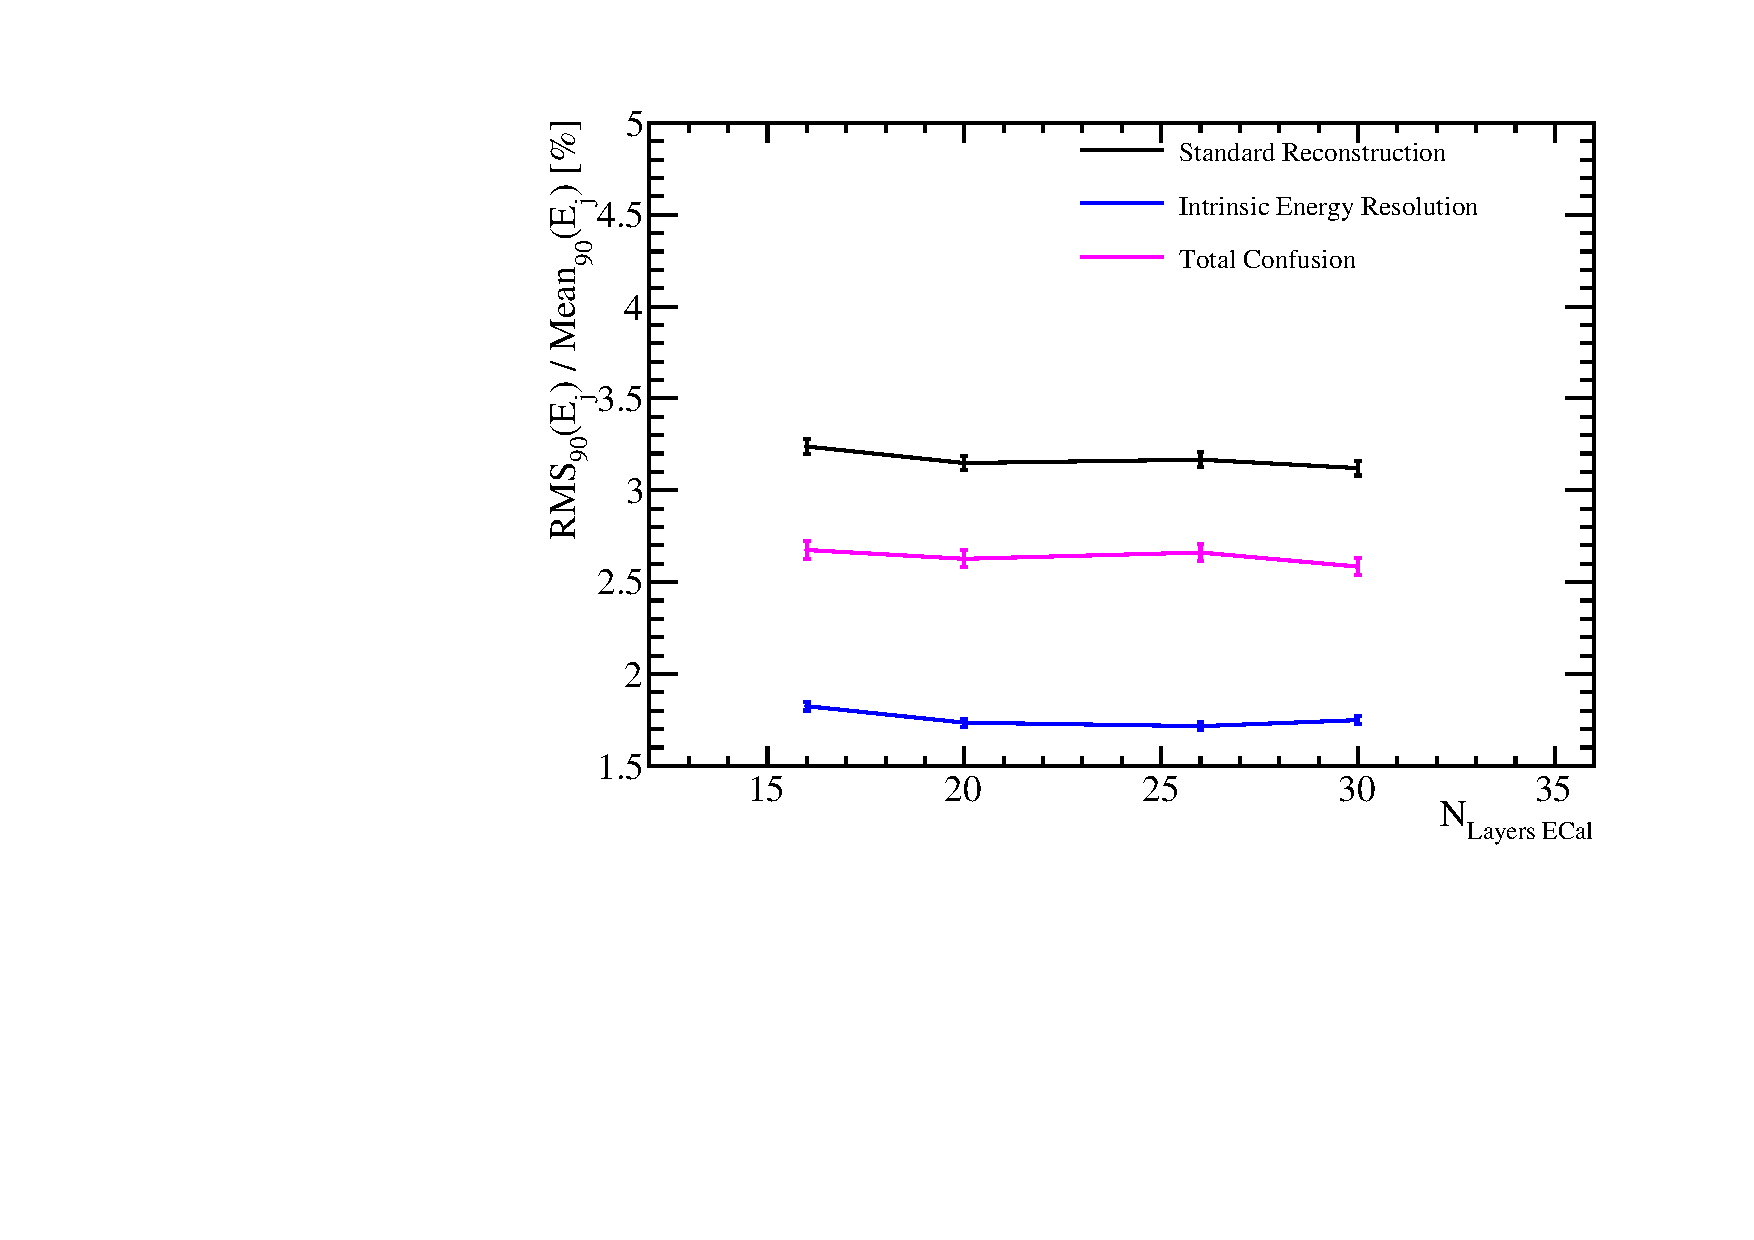
\includegraphics[width=0.5\textwidth]{OptimisationStudies/Plots/JetEnergyResolutions/JER_vs_ScintillatorECalNumberofLayers_500GeV_DiJet_Breakdown.pdf}}
\caption[Jet energy resolution breakdown as a function of ECal longitudinal granularity for 45 and 250 GeV jets.  Results are given for both the silicon and scintillator ECal options.]{Jet energy resolution breakdown as a function of ECal longitudinal granularity for 45 and 250 GeV jets.  Results are given for both the silicon and scintillator ECal options.}
\label{fig:ecalnlayersbreak}
\end{figure}

The strong dependancy of the jet energy resolution on the ECal longitudinal granularity can be expanded upon by looking at the decomposition of the jet energy resolution, which is shown in figure \ref{fig:ecalnlayersbreak} for the 45 and 250 GeV energy jets.  At low energies the trend is twofold: an improvement to the intrinsic energy resolution with more sampling of particle showers and a reduction in the impact of confusion.  For high energy jets, where confusion dominates, there is little to no change in the intrinsic energy resolution and confusion as a function of ECal transverse granularity.  

\begin{figure}
\centering
\subfloat[Silicon active material, 100 GeV $\gamma$.]{\label{fig:ecalsinlayers100gamma}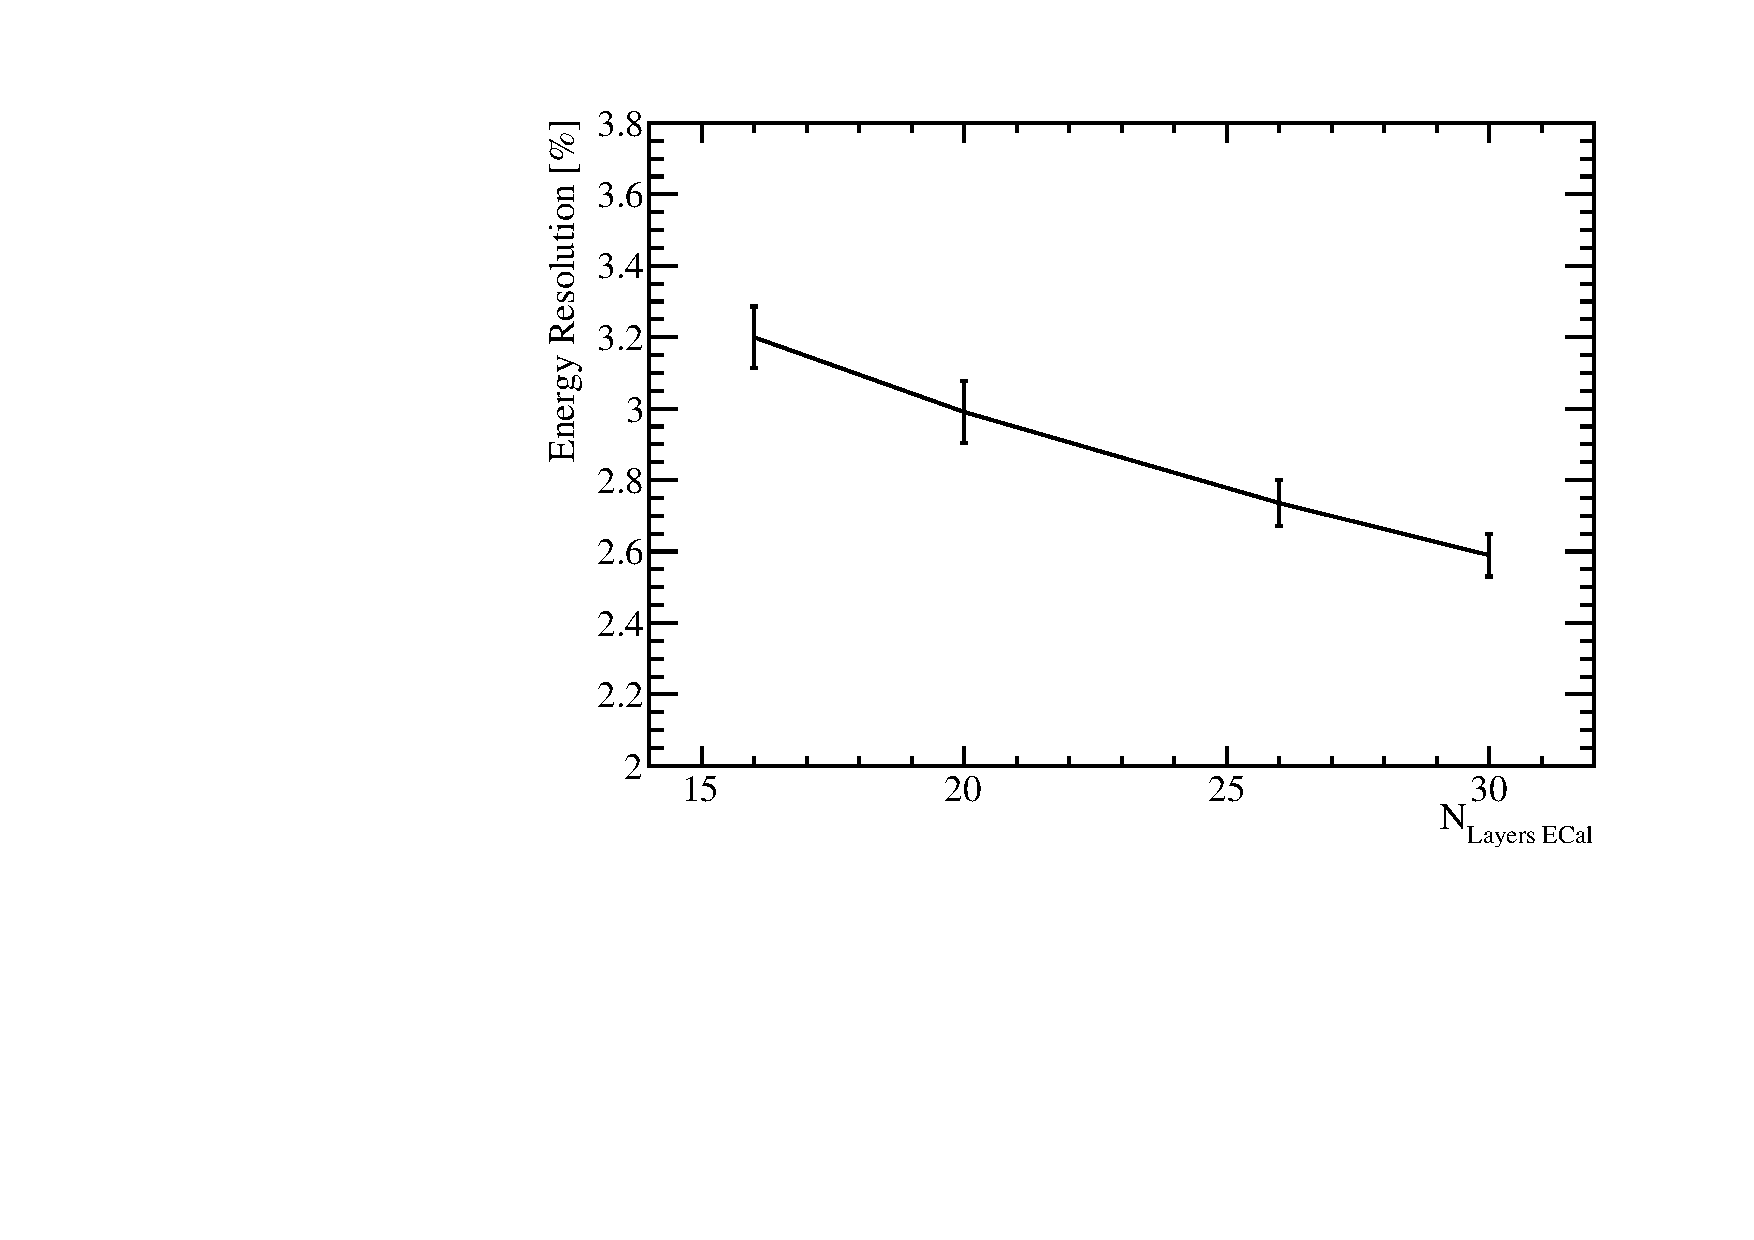
\includegraphics[width=0.5\textwidth]{OptimisationStudies/Plots/EnergyResolution/SiECal100GeVPhotonResVsLayerNumber.pdf}}
\subfloat[Scintillator active material, 100 GeV $\gamma$.]{\label{fig:ecalscnlayers100gamma}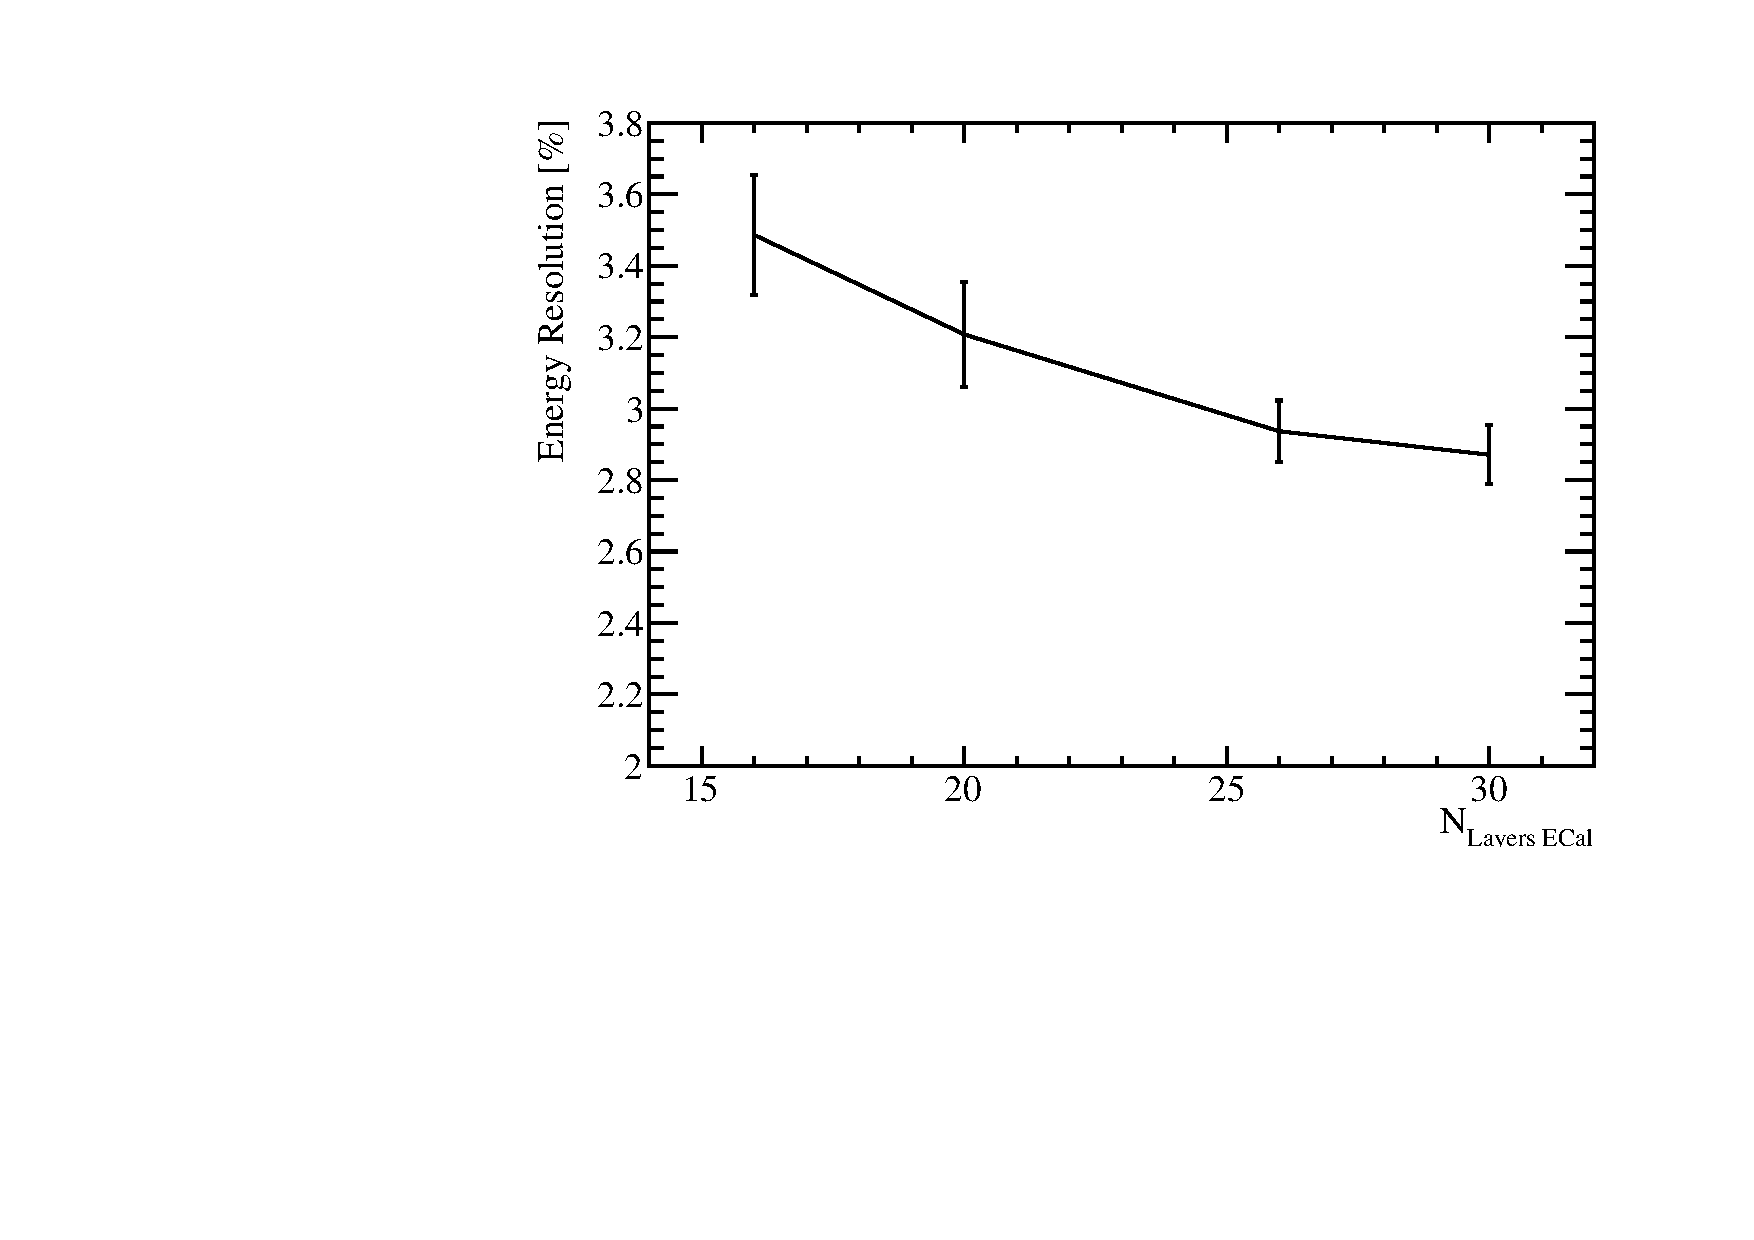
\includegraphics[width=0.5\textwidth]{OptimisationStudies/Plots/EnergyResolution/ScECal100GeVPhotonResVsLayerNumber.pdf}}
\caption[Energy resolution as a function of ECal longitudinal granularity for 100 GeV photons.  Results are given for both the silicon and scintillator ECal options.]{Energy resolution as a function of function of ECal longitudinal granularity for 100 GeV photons.  Results are given for both the silicon and scintillator ECal options.}
\label{fig:ecalnlayersgamma}
\end{figure}

Further understanding is gained by considering the energy resolution of single photon samples at 100 GeV as a function of the longitudinal granularity in the ECal, which is shown in figure \ref{fig:ecalnlayersgamma}.  At these large photon energies it is clear that the intrinsic energy resolution of the ECal is improved by having finer longitudinal segmentation in the ECal.  This trend will be present in the jet energy resolution study, but as only $\approx 10\%$ of the jet energy is measured in the ECal in comparison to $\approx 100\%$ of the photons energy, it will be obscured by the energy resolution of the rest of the detector, which is invariant to the ECal longitudinal segmentation.    

The intrinsic energy resolution of the ECal is improved by having a finer transverse granularity.  This is evident when looking at the energy resolution of photons whose energy deposits are localised within the ECal.  This trend is again clear when considering the energy resolution of low energy jets, however, at higher energies the longitudinal granularity in the ECal is not a significant factor in determining detector performance.

\subsection{ECal Active Material}
In sections \ref{sec:ecalcells} and \ref{sec:ecalnlayers} the performance of the ECal was reported for both the silicon and scintillator options and to a large extent the performance of the two options was the same.  There were a few differences, which attention should be brought to:

\begin{itemize}
\item The intrinsic energy resolution of a silicon ECal is worse than that of a scintillator ECal for low energies, while the trend is reversed at high energies.  The cross over point in performance occurs between 20 and 50 GeV.  This trend is shown in figure \ref{fig:ecalnominalres}.    
\item The "dead" region due to the presence of the MPPC in the scintillator option degrades performance of the detector for small transverse granularities.  No such effect is seen for the silicon option.  This effect is shown in figure \ref{fig:ecalcellsizegamma}.
\end{itemize}

The lack of this "dead" region of the detector and the beneficial intrinsic energy resolution at large energies indicates a preference for a silicon detector, however, there is no clear preference based on these studies.  

%========================================================================================
%========================================================================================

\section{Hadronic Calorimeter Optimisation}
The HCal is designed to measure the energy deposits from hadrons.  The default ILD detector model HCal, summarised in table \ref{table:defaultildhcal}, contains $\approx 6$ nuclear interaction lengths ($\lambda_{I}$).  The ECal contributes approximately one $\lambda_{I}$ giving a total of $\approx 7 \lambda_{I}$, which is sufficient to confine the bulk of jets up to 1 TeV events, which is the maximum running energy for the ILC.  The longitudinal structure of this model consists of 48 readout layers each containing a 3 mm active layer of scintillator and a 20 mm absorber layer of iron.  There are several readout technology options under consideration for the HCal, which are analogue, digital and semi-digital, however, for this study only the analogue HCal is considered.  

\begin{table}[h!]
\centering
\begin{tabular}{ l l}
\hline
Parameter & Default Value \\
\hline
Transverse Granularity & $30 \times 30 \text{mm}^{2}$ square cells \\
Longitudinal Granularity & 48 Readout Layers \\
Active Material Choice & Scintillator Tiles  \\
Active Material Thickness & 3 mm  \\
Absorber Material Choice & Steel \\
Absorber Material Thickness & 20 mm \\
\hline
\end{tabular}
\caption[Nominal ILD detector model HCal configuration.]{Nominal ILD detector model HCal configuration.}
\label{table:defaultildhcal}
\end{table}

% Nuclear interaction length iron 167.7mm
% Nuclear interaction length tungsten 99.46mm 
% Nuclear interaction length silicon 465.2mm 
% Nuclear interaction length polystyrene 770.7mm

The parameters being optimised in this study are:
\begin{itemize}
\item Transverse granularity or cell size.  This is key to successful application of pattern recognition in the particle flow paradigm, but should not change intrinsic energy resolution.   
\item Longitudinal granularity or cell depth.  This governs the intrinsic energy resolution of a calorimeter.
\item Depth of calorimeter.  This is important in determining the impact of leakage of energy out of the detector.  
\item Sampling fraction.  This is the ratio of the active medium thickness to the absorber medium thickness.  As sampling calorimetry is based on sampling of particle showers it is expected that this is an important parameter.  However, above a given sampling fraction there should be little difference between performance if showers are sampled at a high enough rate to get a good estimate of the incoming particles energy.
\item Absorber material choice.  This is a choice between steel or tungsten.  While this does not change the active medium choice it does dictate the growth and propagation of showers and so plays a crucial role in calorimetry.  While tungsten is more expensive than steel for the raw material the larger number of interaction lengths per length scale for tungsten mean that it is possible to create a smaller detector with the same number of interaction lengths within it.  This reduces the size of the solenoid needed to generate the magnetic field and so lowers the price of the detector.  As both of these materials are viable as absorber medium choices it is crucial to determine if either is more advantageous from a physics perspective.  
\end{itemize}

%========================================================================================

\subsection{HCal Absorber Material}
\label{sec:hcalabsorbermaterial}
The nominal choice of absorber material is steel, tungsten provides a feasible alternative material.  While more expensive than steel, tungsten contains more radiation lengths per unit length than steel and so the overall size of the detector would reduce meaning the solenoid could be smaller, which would to first order offset the additional cost of the tungsten.  This section aims to determine whether either of these options is beneficial when considering the jet energy resolution of the detector.

In this study the total depth of absorber material, in nuclear interaction lengths, was held constant for both models.  This was to ensure any performance changes were not due to additional material as opposed to the intrinsic energy resolutions of the absorber materials.  The interaction of hadrons with the absorber material within the detector is simulated by GEANT4.  The model for these interactions is dependent upon the choice of physics list, which by default is the QGSP\_BERT physics list.  This list is recommended by the GEANT4 authors to use for high energy physics calorimetry as it gives good agreement between experiment.  For this study both the QGSP\_BERT and the QGSP\_BERT\_HP physics lists are tested.  The QGSP\_BERT\_HP list uses the high precision neutron package (NeutronHP) to deal with the transportation of neutrons from below 20 MeV to thermal energies.  This added detail was thought to be necessary for a study involving tungsten due to the increased time of shower development.    

The jet energy resolution for the steel and the tungsten HCal options, for using both the QGSP\_BERT and the QGSP\_BERT\_HP physics lists, are shown in figure \ref{fig:hcalabsmaterial}.  These results indicate that steel outperforms tungsten as an absorber material, particularly for high energy jets.  At low energies the performance is similar, indicating that the intrinsic energy resolution of the two options is comparable.  The use of the QGSP\_BERT\_HP physics list, as opposed to QGSP\_BERT, has a minimal impact on these results.

\begin{figure}
\centering
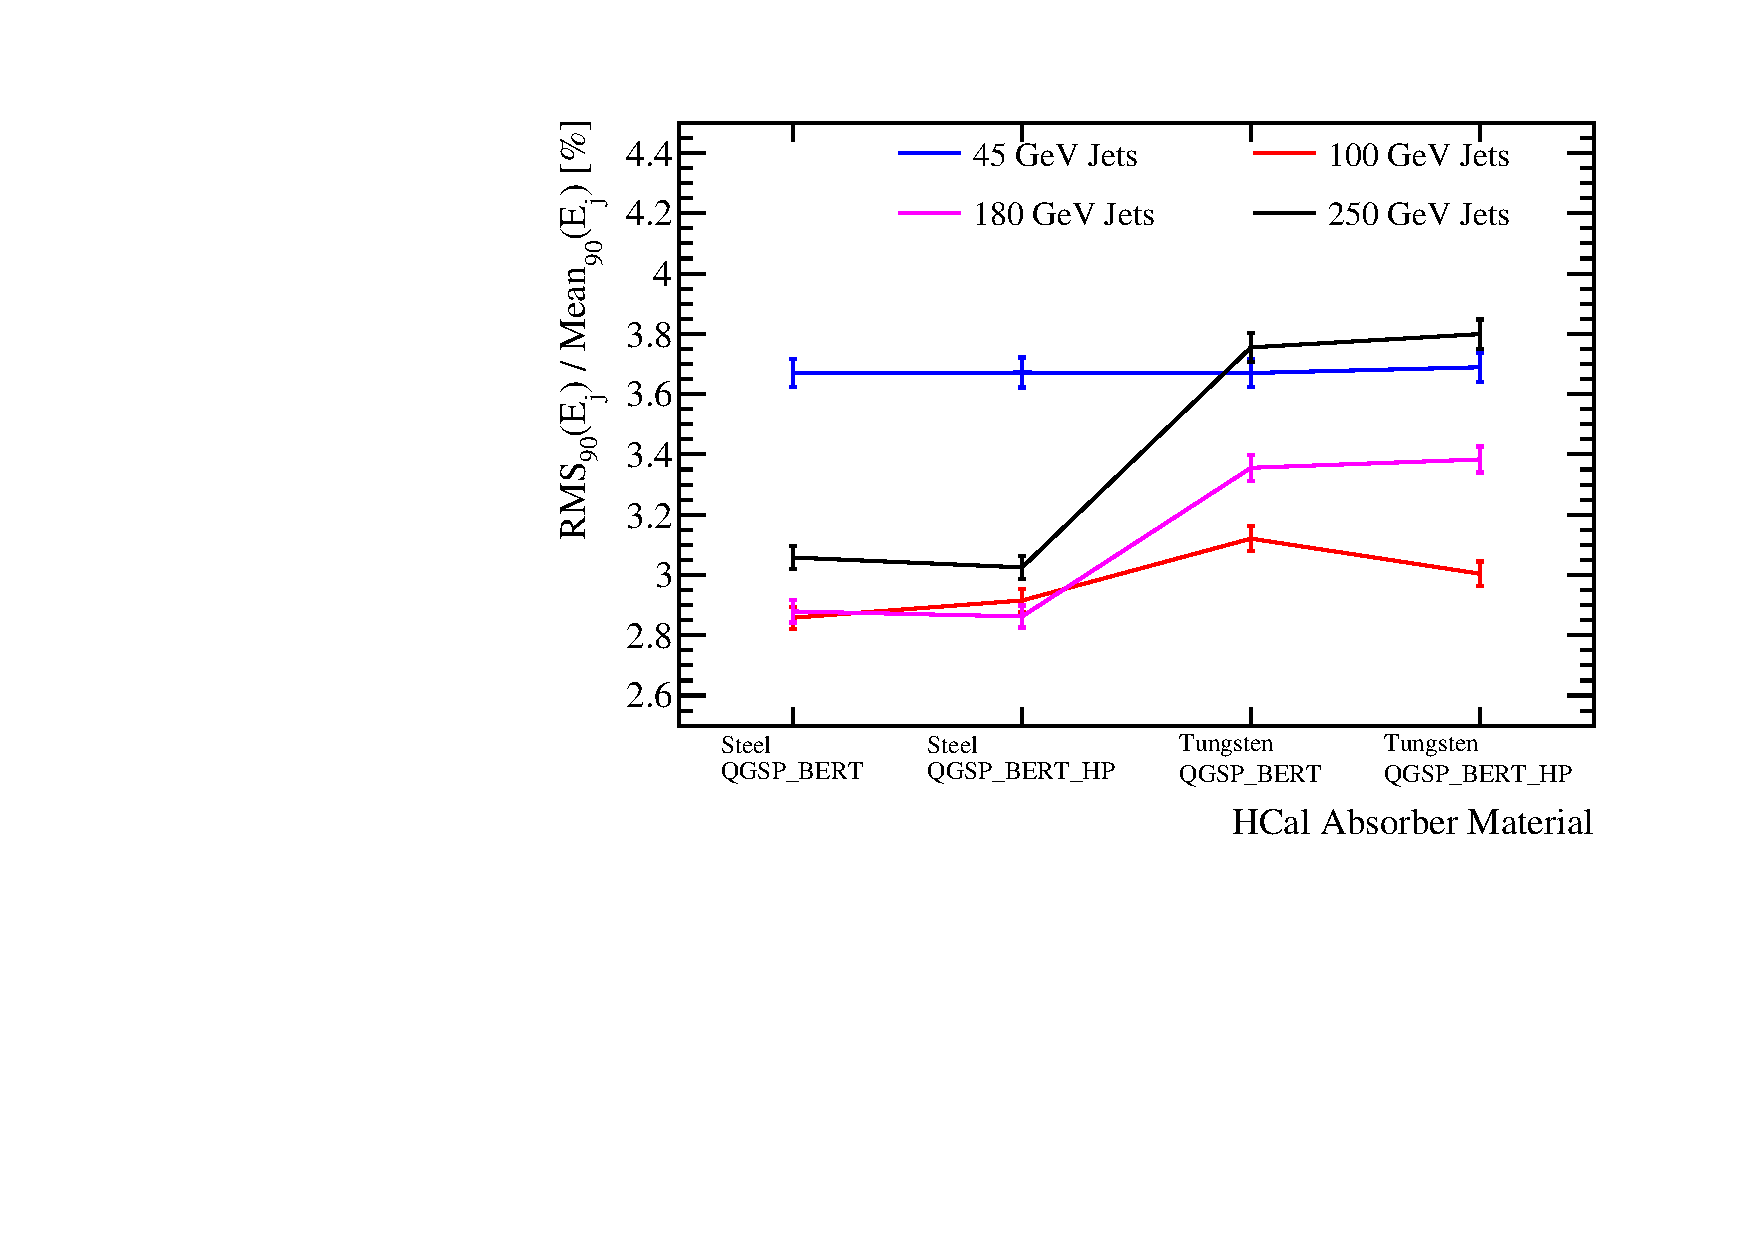
\includegraphics[width=0.5\textwidth]{OptimisationStudies/Plots/JetEnergyResolutions/JER_vs_HCalAbsorberMaterial.pdf}
\caption[Jet energy resolution as a function of absorber material in the HCal and physics list.]{Jet energy resolution as a function of absorber material in the HCal and physics list.}
\label{fig:hcalabsmaterial}
\end{figure} 

Expanding upon this further by examining the jet energy resolution breakdowns as shown in figure \ref{fig:hcalabsmaterialbreak}, it can be seen that the change in performance when changing the HCal absorber material from steel to tungsten is due to changes in the confusion.  The change in confusion is most likely due to the fact that the PandoraPFA algorithms are tuned for HCal cell dimensions based on the steel HCal option, while the HCal cells for the tungsten option HCal will be smaller by a factor of approximately 1.7 ($\approx 16.77/9.946$).  The jet energy resolution breakdowns also indicate that the intrinsic energy resolution of the tungsten HCal is marginally worse, particularly for high energy jets, than that of a steel HCal.  Therefor, even if the algorithms were fully optimised for the tungsten option such that the confusion terms for the two options were comparable the performance of the steel HCal would still be preferred over the tungsten option making the steel option the more preferred of the two.  

\begin{figure}
\centering
\subfloat[45 GeV Jets.]{\label{fig:hcalabsmaterial45break}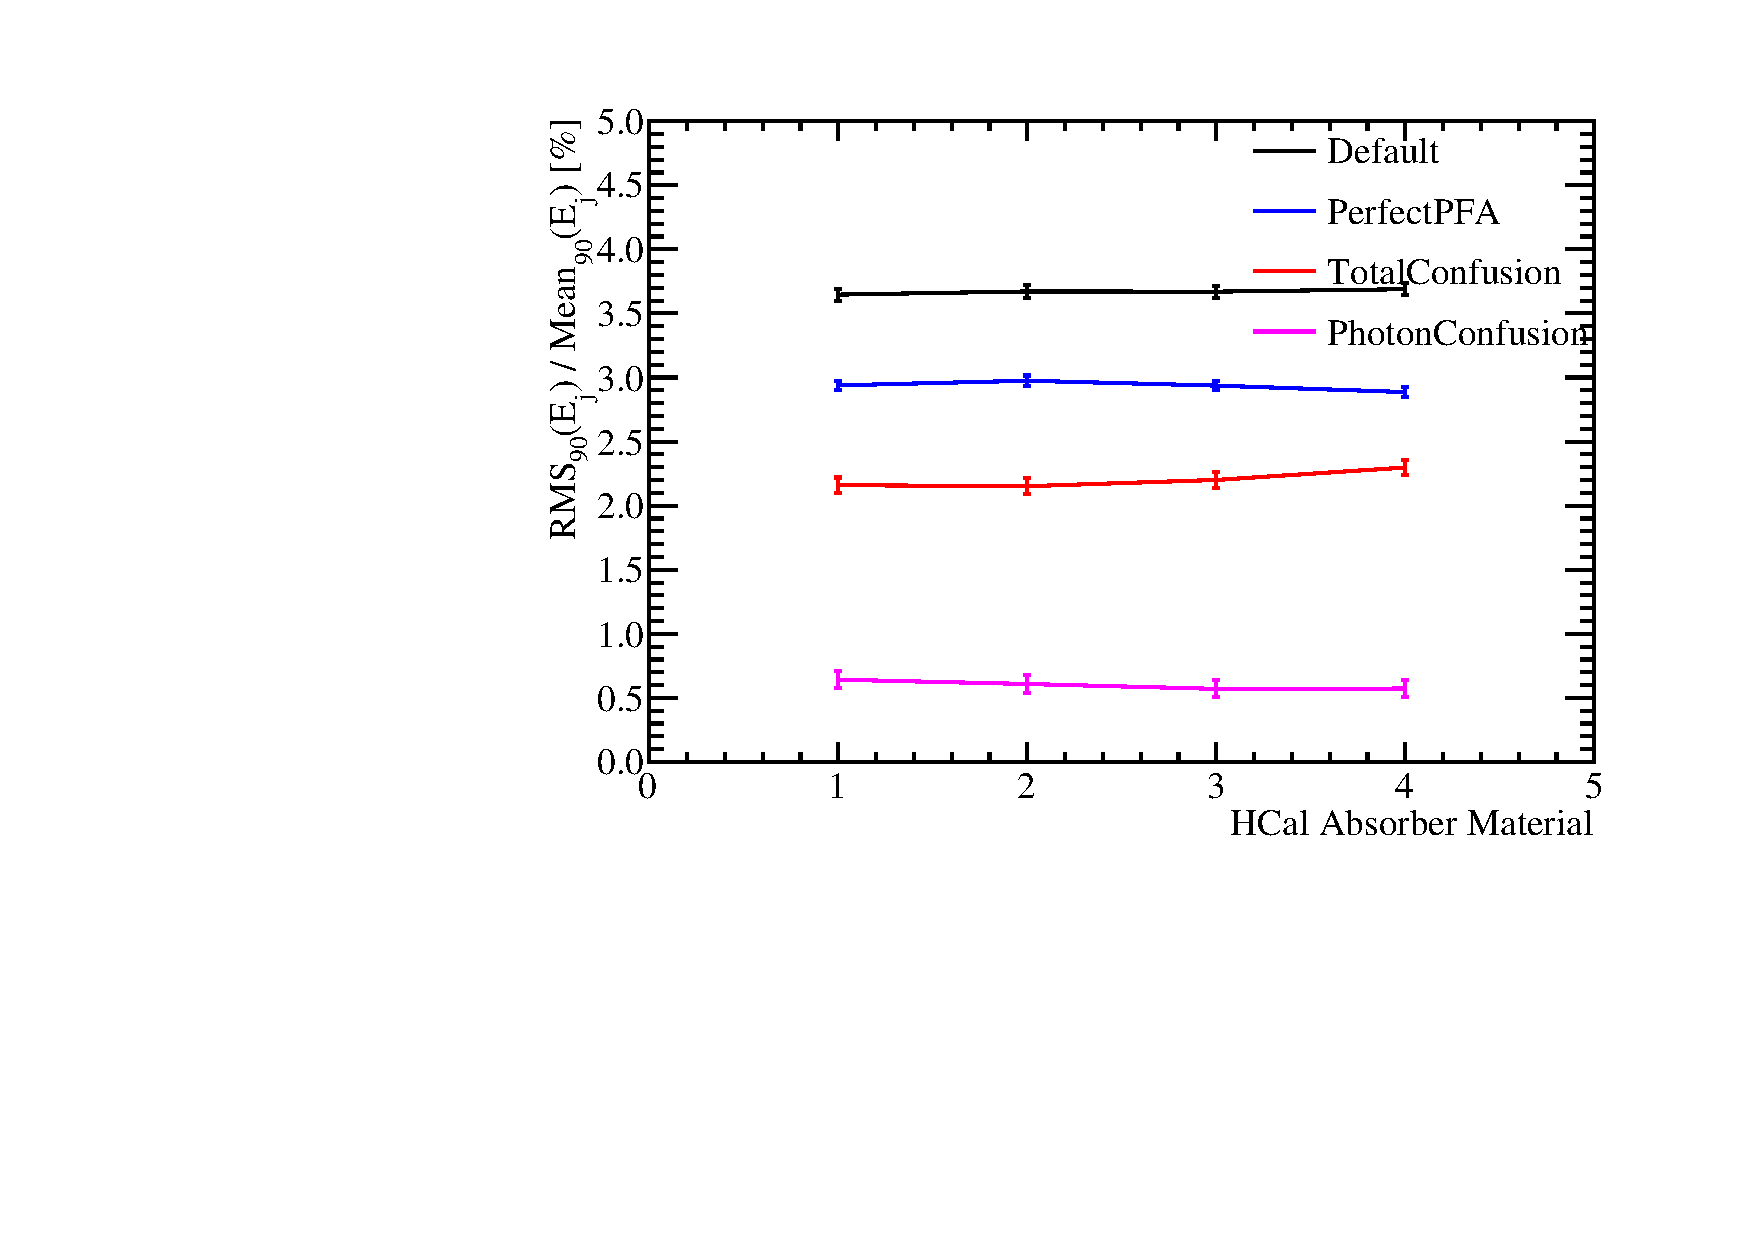
\includegraphics[width=0.5\textwidth]{OptimisationStudies/Plots/JetEnergyResolutions/JER_vs_HCalAbsorberMaterial_91GeV_DiJet_Breakdown.pdf}}
\subfloat[250 GeV Jets.]{\label{fig:hcalabsmaterial250break}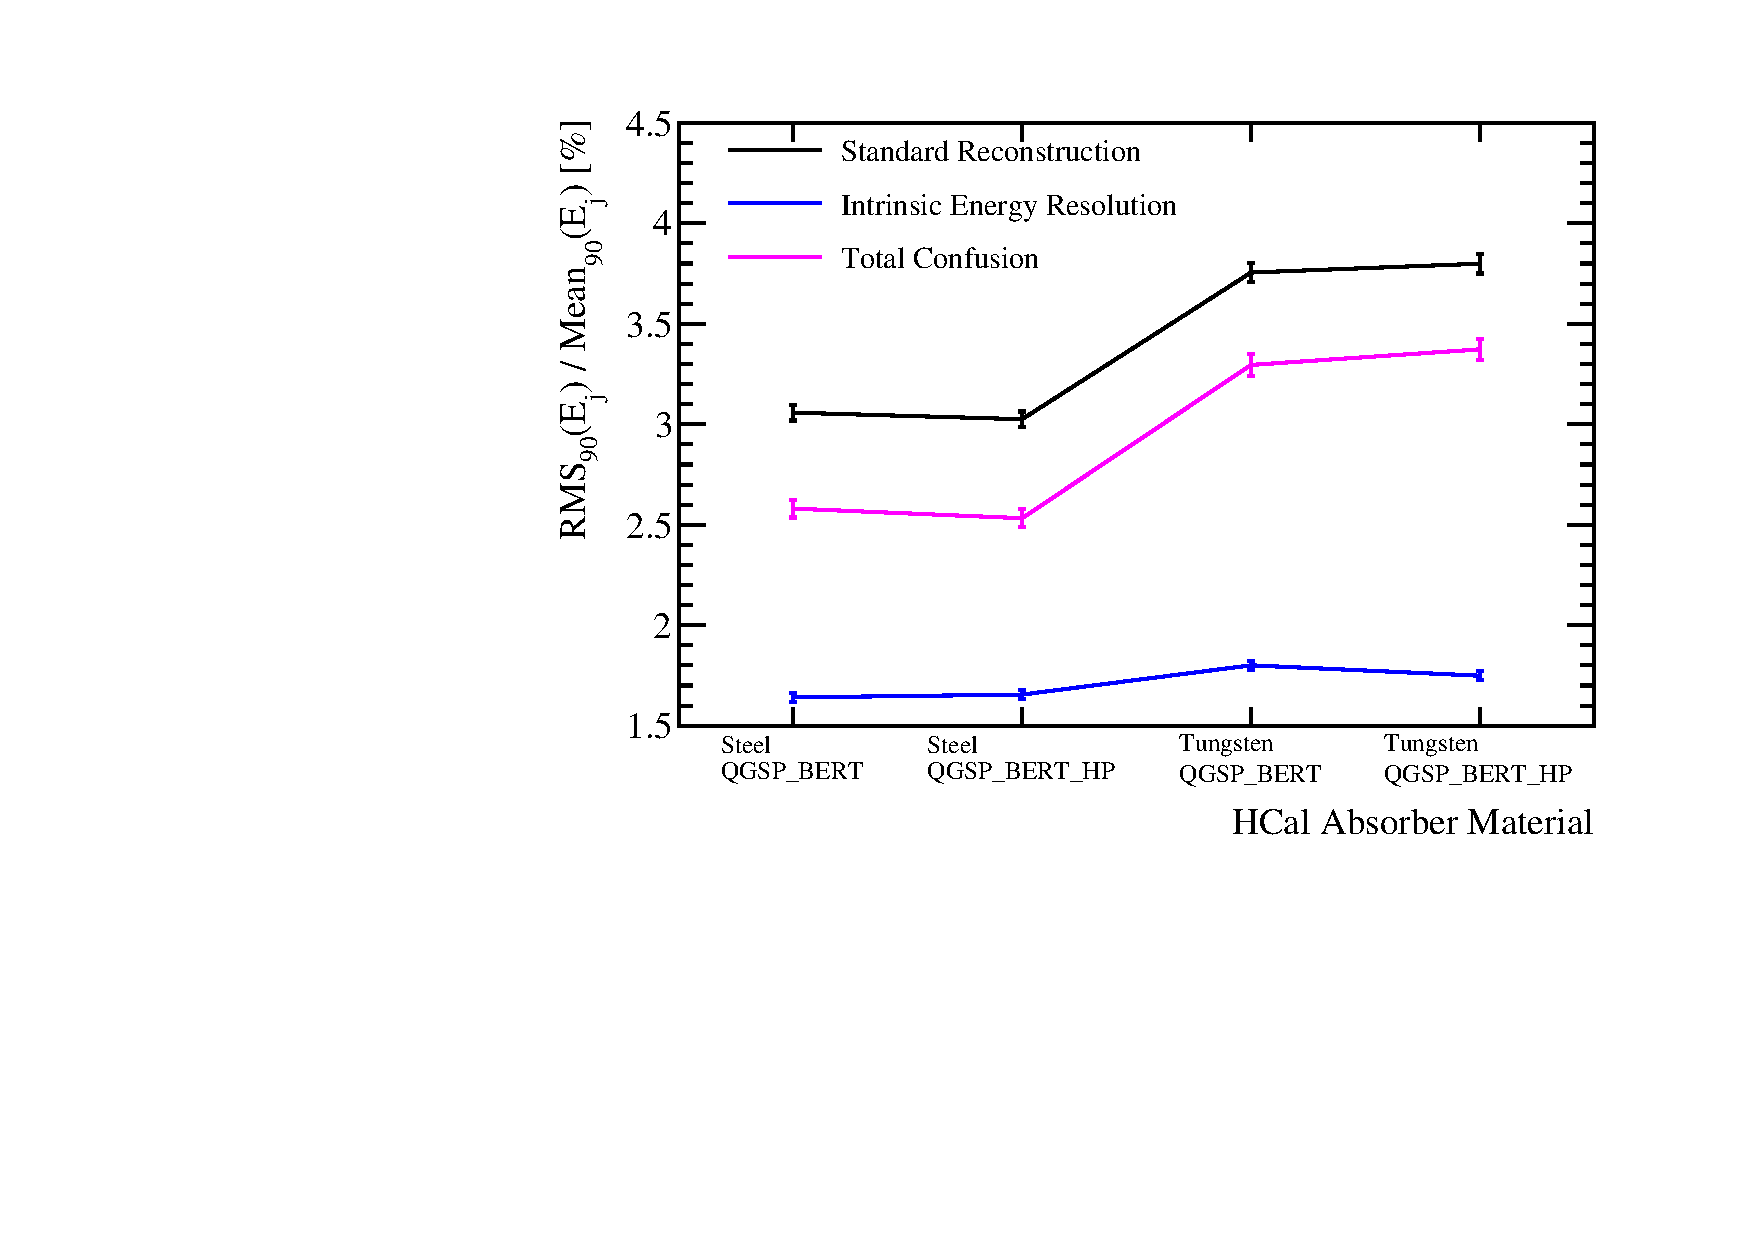
\includegraphics[width=0.5\textwidth]{OptimisationStudies/Plots/JetEnergyResolutions/JER_vs_HCalAbsorberMaterial_500GeV_DiJet_Breakdown.pdf}}
\caption[Jet energy resolution breakdown as a function of HCal absorber material and physics list for 45 and 250 GeV jets.]{Jet energy resolution breakdown as a function of HCal absorber material and physics list for 45 and 250 GeV jets.}
\label{fig:hcalabsmaterialbreak}
\end{figure}

%========================================================================================

\subsection{HCal Transverse Granularity}
\label{sec:hcalcells}
For this study a number of different detector models were considered where the transverse granularity in the HCal had been varied about the nominal value of $30 \times 30 \text{mm}^{2}$ square cells.  The granularities considered were $10 \times 10 \text{mm}^{2}$, $20 \times 20 \text{mm}^{2}$, $30 \times 30 \text{mm}^{2}$, $40 \times 40 \text{mm}^{2}$, $50 \times 50 \text{mm}^{2}$ and $100 \times 100 \text{mm}^{2}$ square cells.  The jet energy resolution as a function of transverse granularity in the HCal is shown in figure \ref{fig:hcalcellsize}.

\begin{figure}
\centering
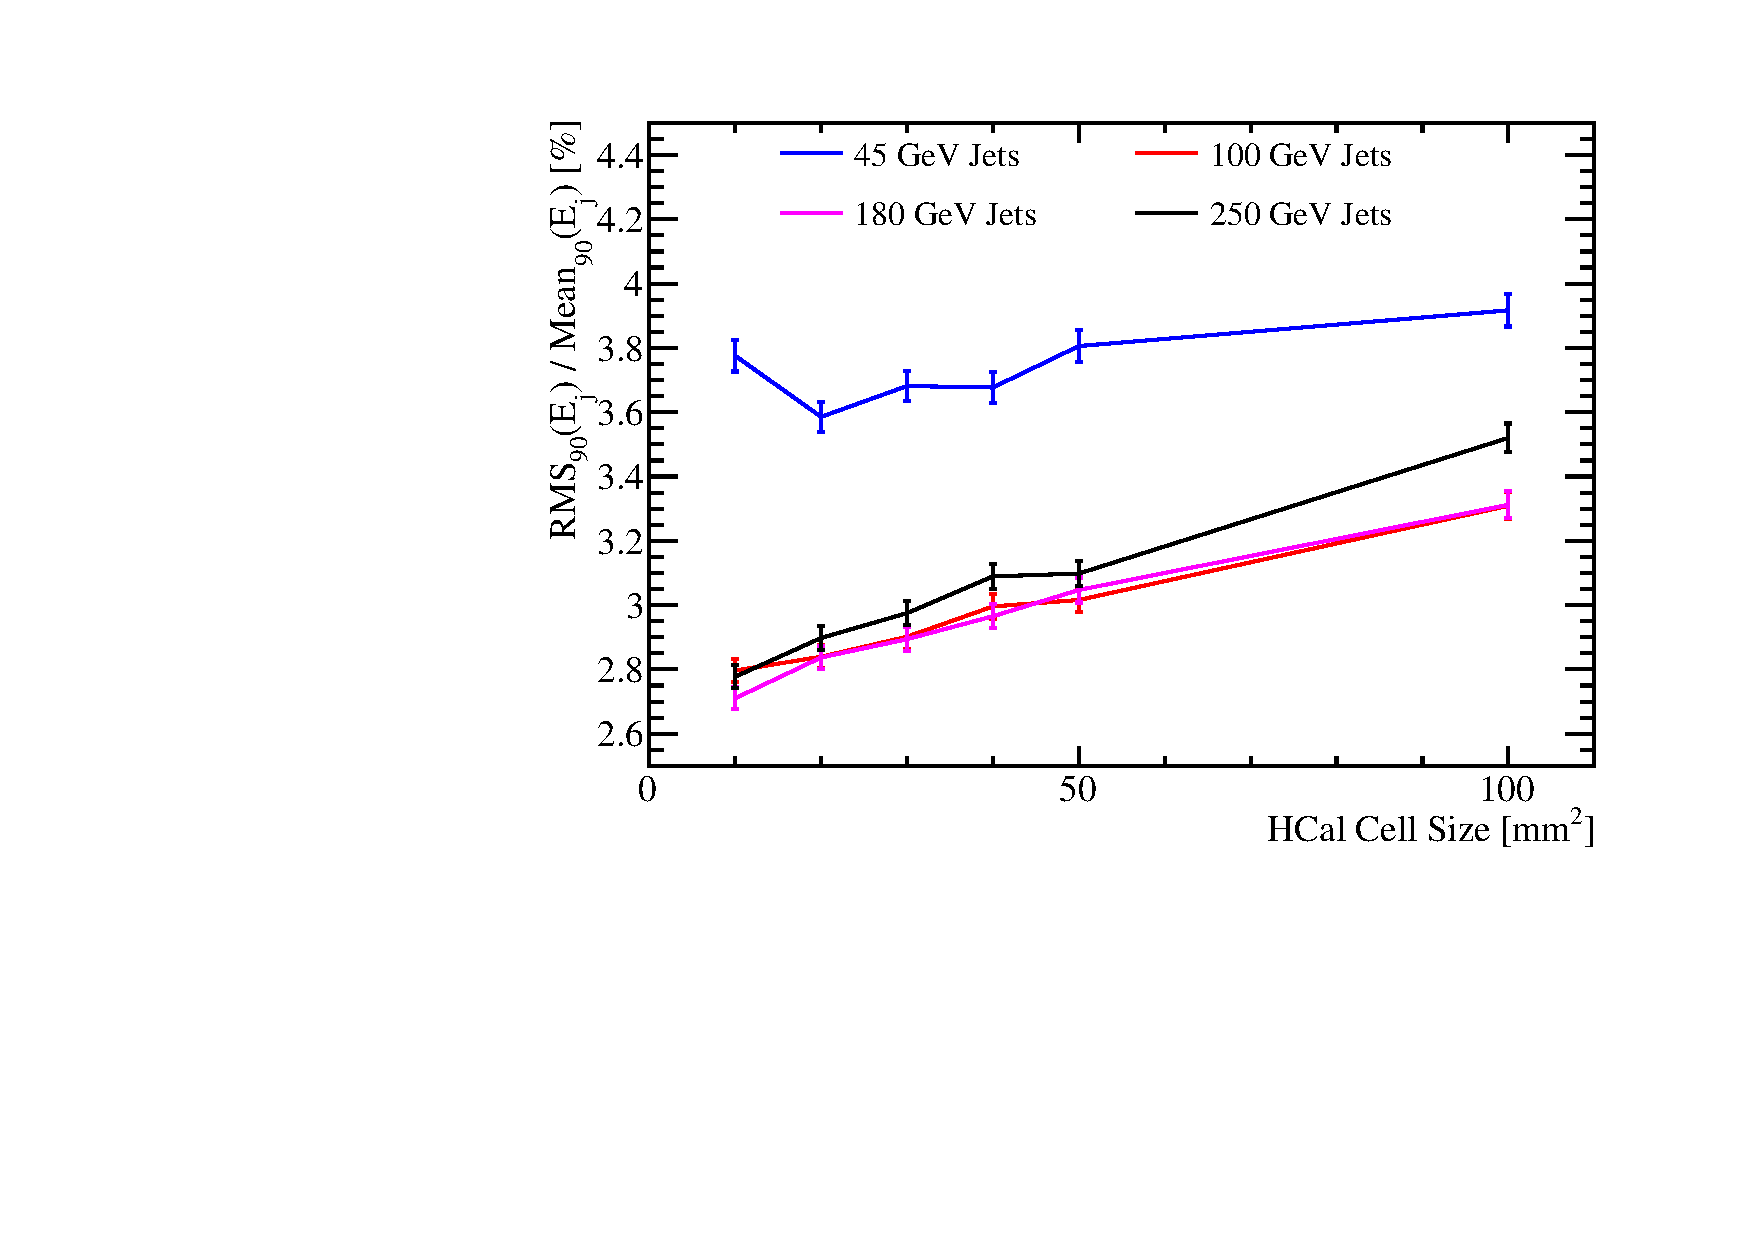
\includegraphics[width=0.5\textwidth]{OptimisationStudies/Plots/JetEnergyResolutions/JER_vs_HCalCellSize.pdf}
\caption[Jet energy resolution as a function of HCal cell size.]{Jet energy resolution as a function of HCal cell size.}
\label{fig:hcalcellsize}
\end{figure}

As with the case for the ECal, the jet energy resolution was found to improve with decreasing cell size as smaller cell size lead to better separation of energy deposits from neutral and charged particle showers.

\begin{figure}
\centering
\subfloat[45 GeV Jets.]{\label{fig:hcalcellsize45break}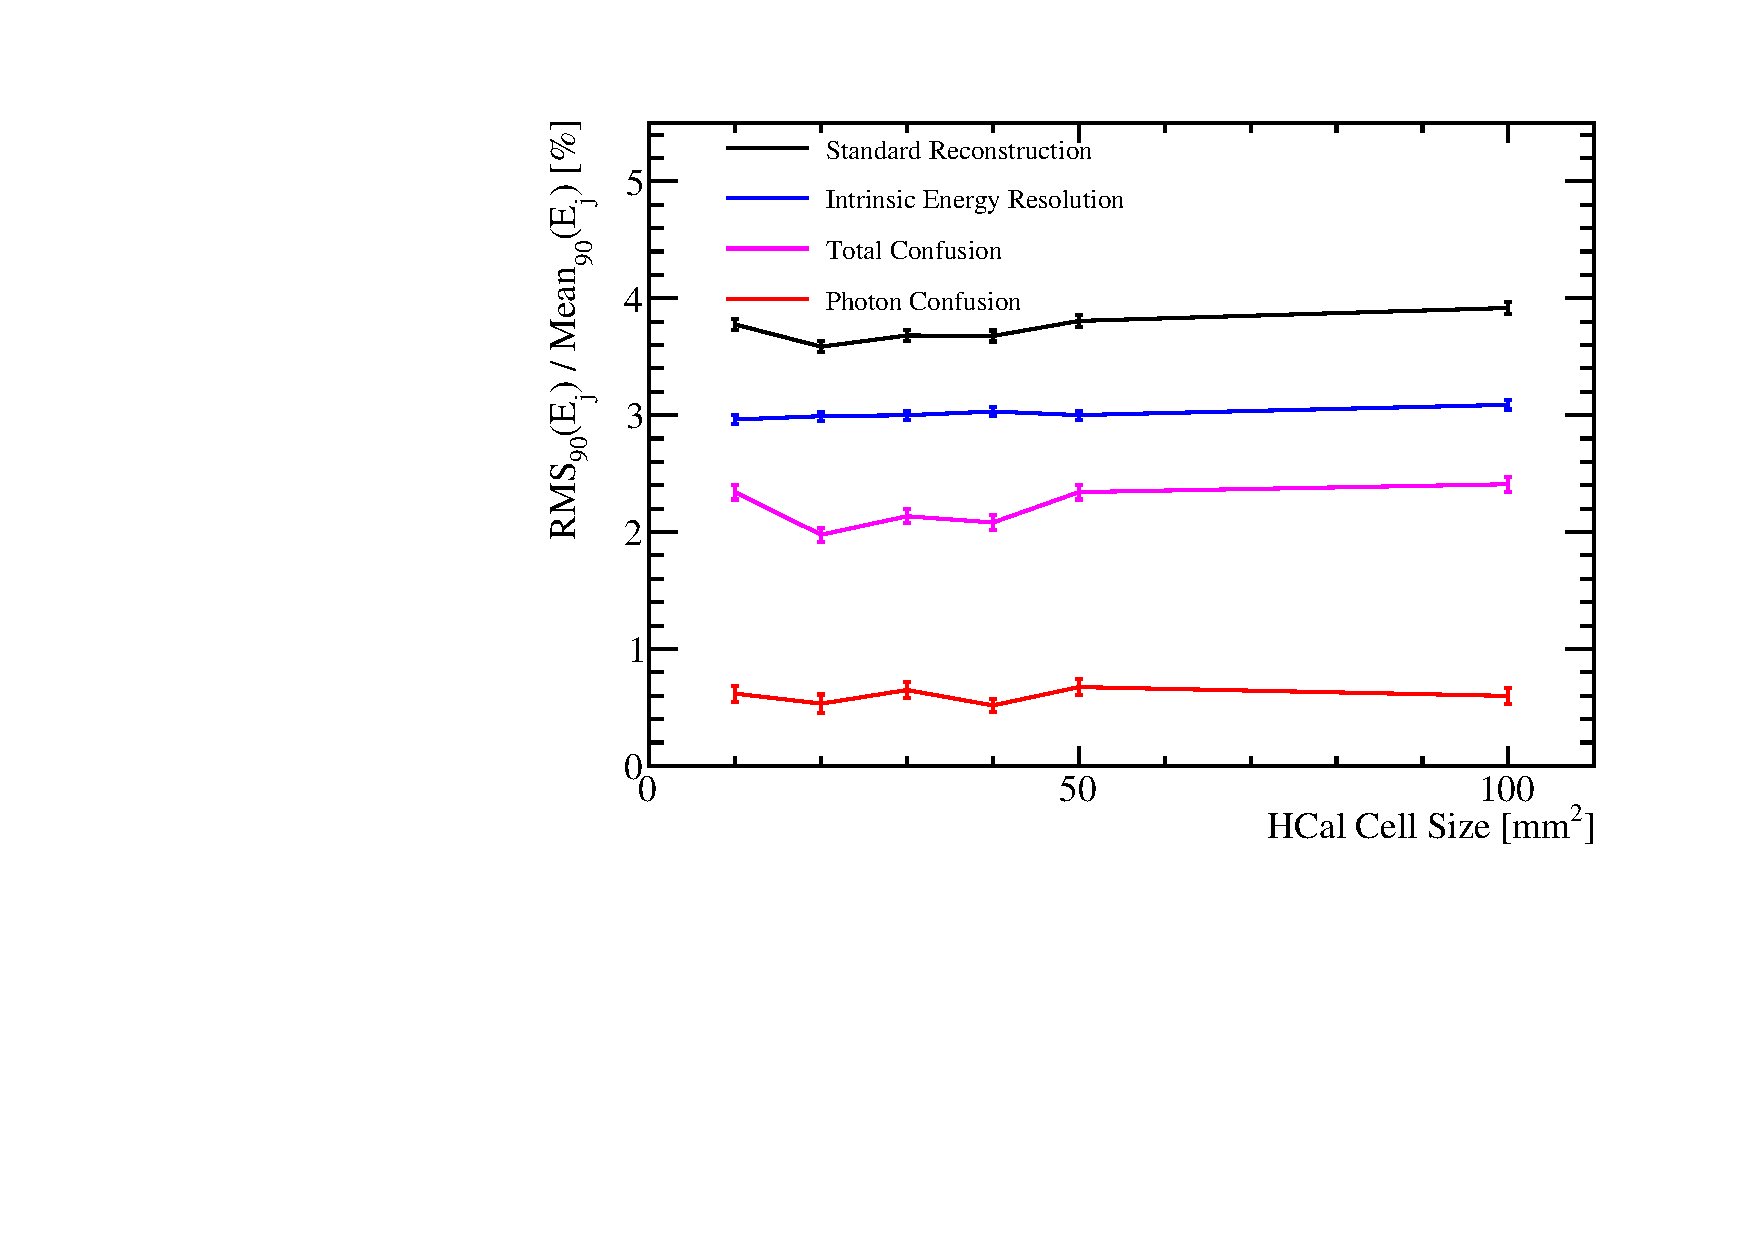
\includegraphics[width=0.5\textwidth]{OptimisationStudies/Plots/JetEnergyResolutions/JER_vs_HCalCellSize_91GeV_DiJet_Breakdown.pdf}}
\subfloat[250 GeV Jets.]{\label{fig:hcalcellsize250break}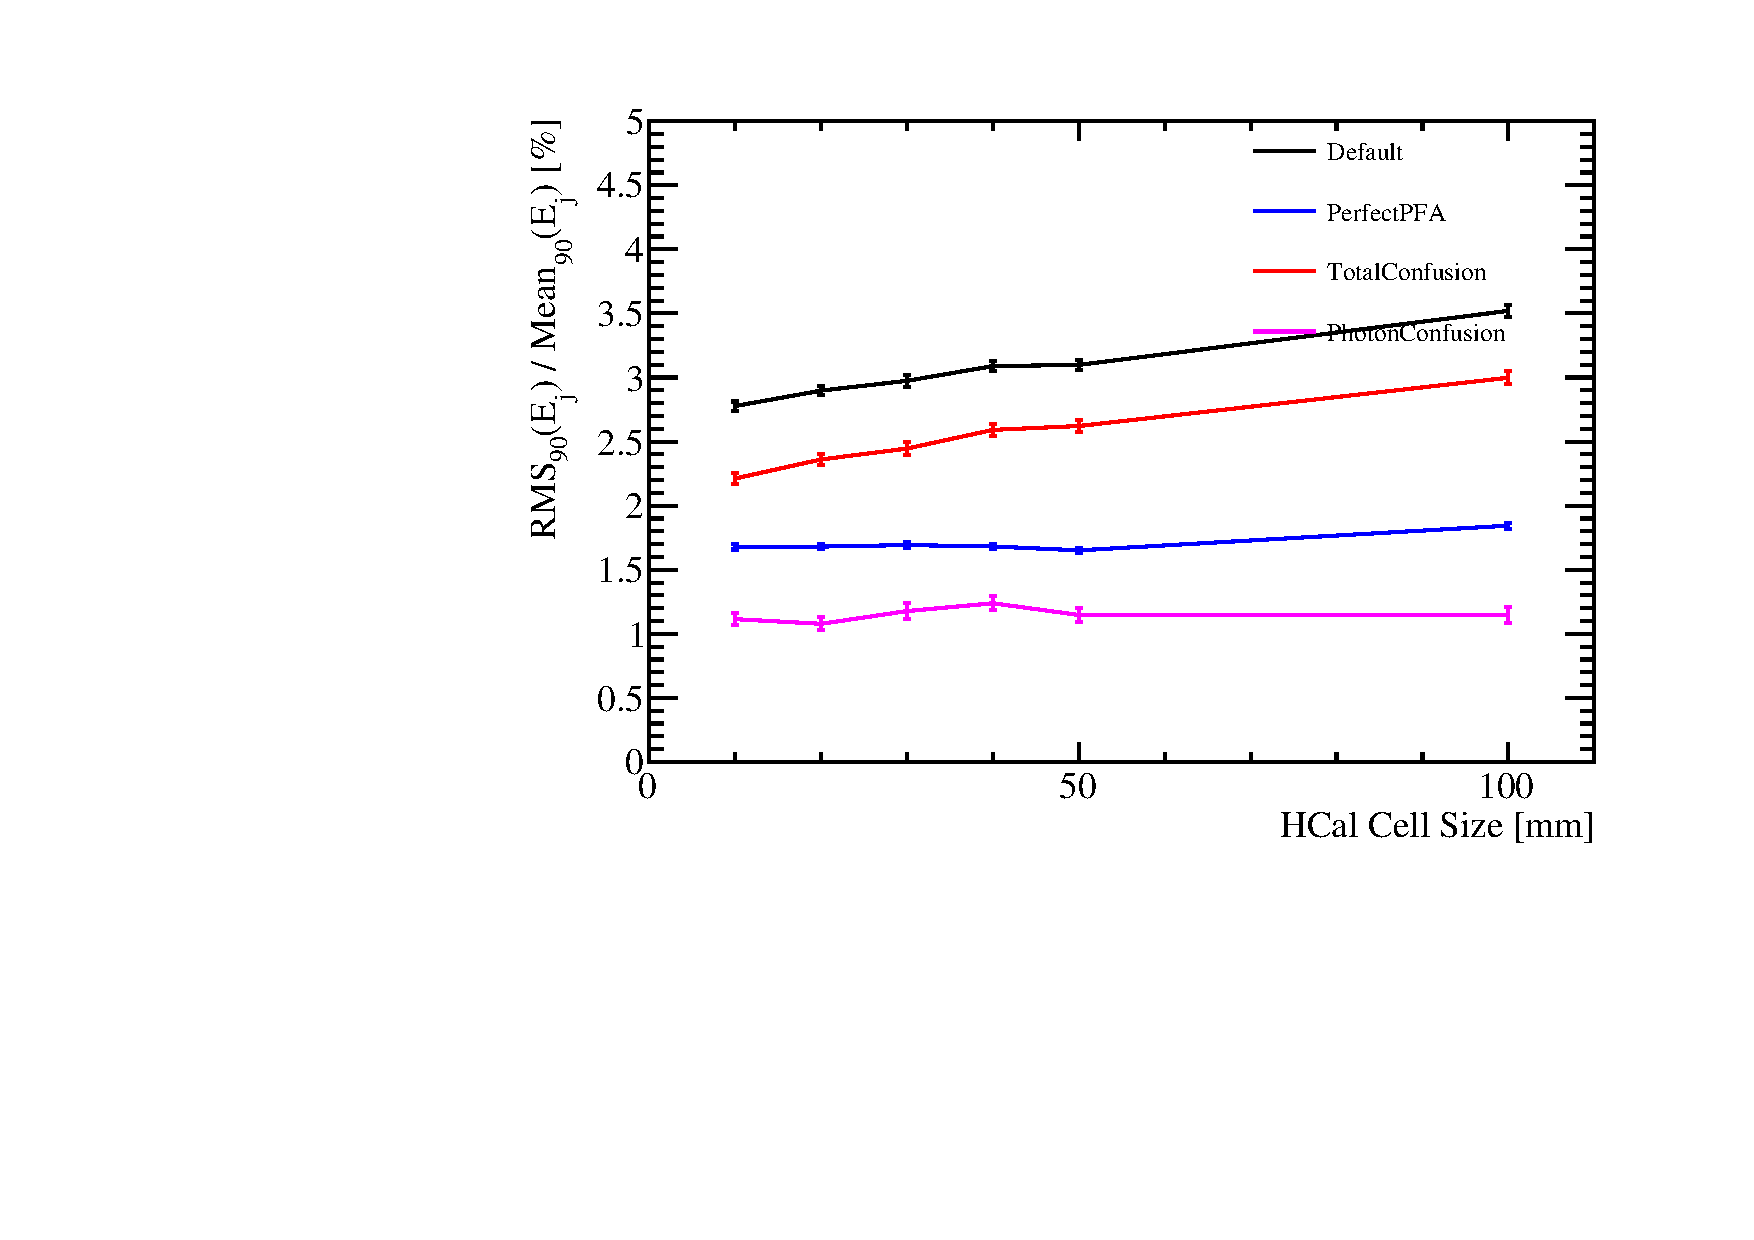
\includegraphics[width=0.5\textwidth]{OptimisationStudies/Plots/JetEnergyResolutions/JER_vs_HCalCellSize_500GeV_DiJet_Breakdown.pdf}}
\caption[Jet energy resolution breakdown as a function of HCal transverse granularity for 45 and 250 GeV jets.]{Jet energy resolution breakdown as a function of HCal transverse granularity for 45 and 250 GeV jets.}
\label{fig:hcalcellsizebreak}
\end{figure}

The jet energy resolution breakdowns, shown in figure, \ref{fig:hcalcellsizebreak}, show that the confusion term varies when changing the HCal transverse granularity, but the intrinsic energy resolution does not.  Furthermore, the photon confusion is invariant to changes in HCal transverse granularity, indicating that the observed overall performance changes are due to the effects of confusion arising from energy deposits from charged and neutral hadrons.  Once again for 45 GeV jets the detector performance is dominated by intrinsic energy resolution and so HCal transverse granularity has little effect, while for 250 GeV jets the performance is dominated by confusion and HCal transverse granularity becomes more significant.  

\begin{figure}
\centering
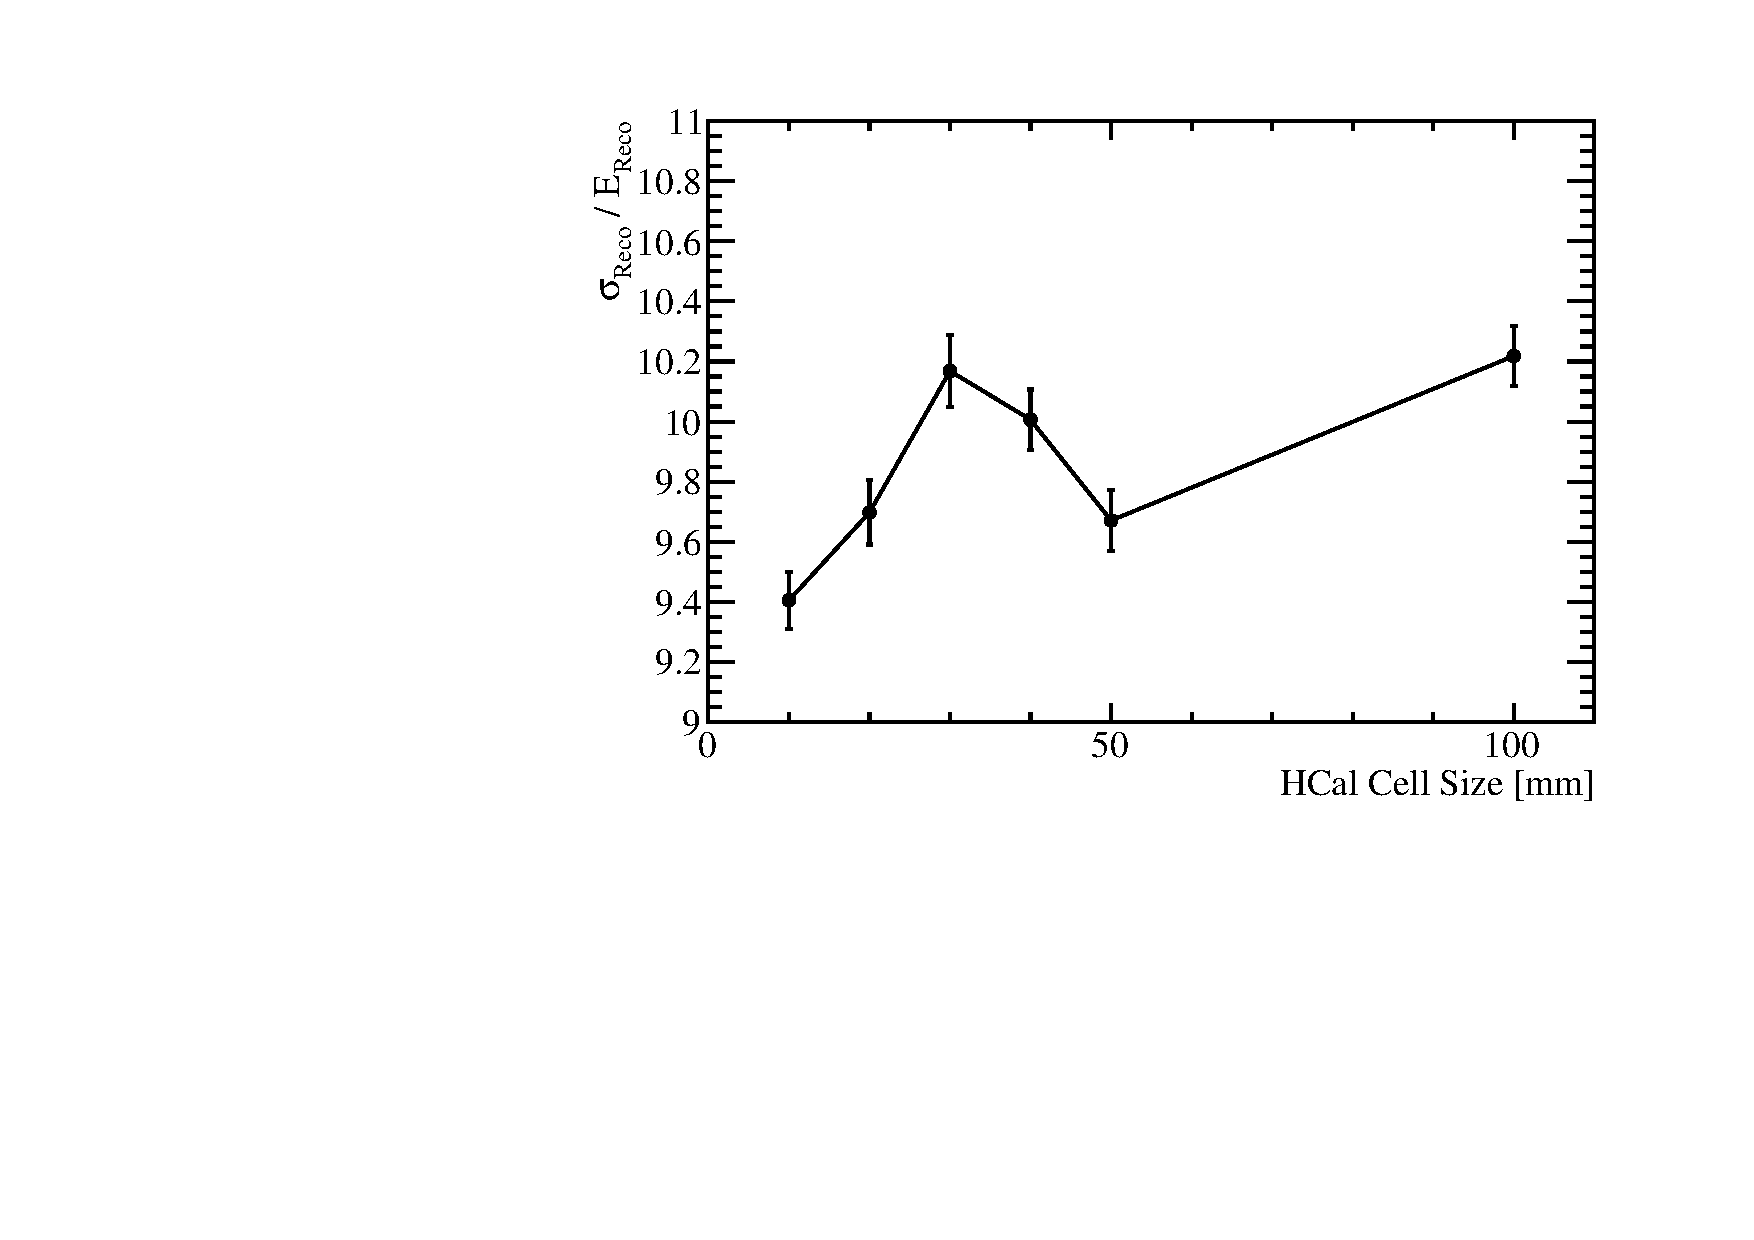
\includegraphics[width=0.5\textwidth]{OptimisationStudies/Plots/EnergyResolution/ER_vs_HCalCellSize_50GeVKaon0L.pdf}
\caption[Energy resolution as a function of HCal transverse granularity for 50 GeV $\text{K}^{0}_{L}$.]{Energy resolution as a function of HCal transverse granularity for 50 GeV $\text{K}^{0}_{L}$.}
\label{fig:hcalcellskaon}
\end{figure}

The energy resolution of single long lived neutral kaons, $\text{K}^{0}_{L}$, at 50 GeV is considered as a function of transverse granularity in the HCal.  This is shown in figure \ref{fig:hcalcellskaon} and, as expected, the energy resolution of the detector is largely invariant to changes in the transverse granularity in the HCal.  As these $\text{K}^{0}_{L}$ samples may deposit energy in the ECal, this figure represents the intrinsic energy resolution of the ILD detector as a whole and not purely that of the HCal.  However, it expected that the bulk of the energy deposited by these samples occurs within the HCal and so such plots are a useful representation of the HCal performance.  

The transverse granularity of the HCal acts to determine the impact of confusion from charged and neutral hadron energy deposits.  It does not vary the intrinsic energy resolution of the detector, nor does it impact the reconstruction of photons.  As confusion is dominant at high jet energies the HCal transverse granularity gains an increasing role in determining detector performance as the energy in an event increases. 

%========================================================================================

\subsection{HCal Longitudinal Granularity}
\label{sec:hcalnlayers}

MAKE THIS SECTIONS ABOUT ADDING LAYERS TO HCAL

%========================================================================================

\subsection{HCal Sampling Fraction}
\label{sec:hcalsamplingfraction}


%========================================================================================

\subsection{HCal Sampling Frequency}
\label{sec:hcalsamplingfrequency}
A number of detector models were examined where the longitudinal segmentation of the HCal, of fixed total thickness, had been varied about the nominal value.  In all cases the absorber material was steel while the active material was scintillator.  Each HCal configuration had the same total number of nuclear interaction lengths, 5.72 $\lambda_{I}$ in the absorber material and 0.19 $\lambda_{I}$ in the active material, however, the thickness of the layers was varied depending on the total number of layers being considered.  The ratio of the active material layers to the absorber material layers, the sampling fraction, was also kept constant in this study.  A summary of the detector models considered in this study can be found in table \ref{table:nlayershcaloption}.  

\begin{table}[h!]
\centering
\begin{tabular}{ l l l }
\hline
Number $N_{\text{Layers HCal}}$& Absorber Thickness & Active Thickness \\
 & [mm] & [mm] \\
\hline
60 & 16.00 & 2.40 \\ 
54 & 17.78 & 2.67 \\
48 & 20.00 & 3.00 \\
42 & 22.86 & 3.43 \\
36 & 26.67 & 4.00 \\
30 & 32.00 & 4.80 \\
24 & 40.00 & 6.00 \\
18 & 53.33 & 8.00 \\
\hline
\end{tabular}
\caption[Transverse granularity layout of various HCal models considered.]{Transverse granularity layout of various HCal models considered.}
\label{table:nlayershcaloption}
\end{table}

\begin{figure}
\centering
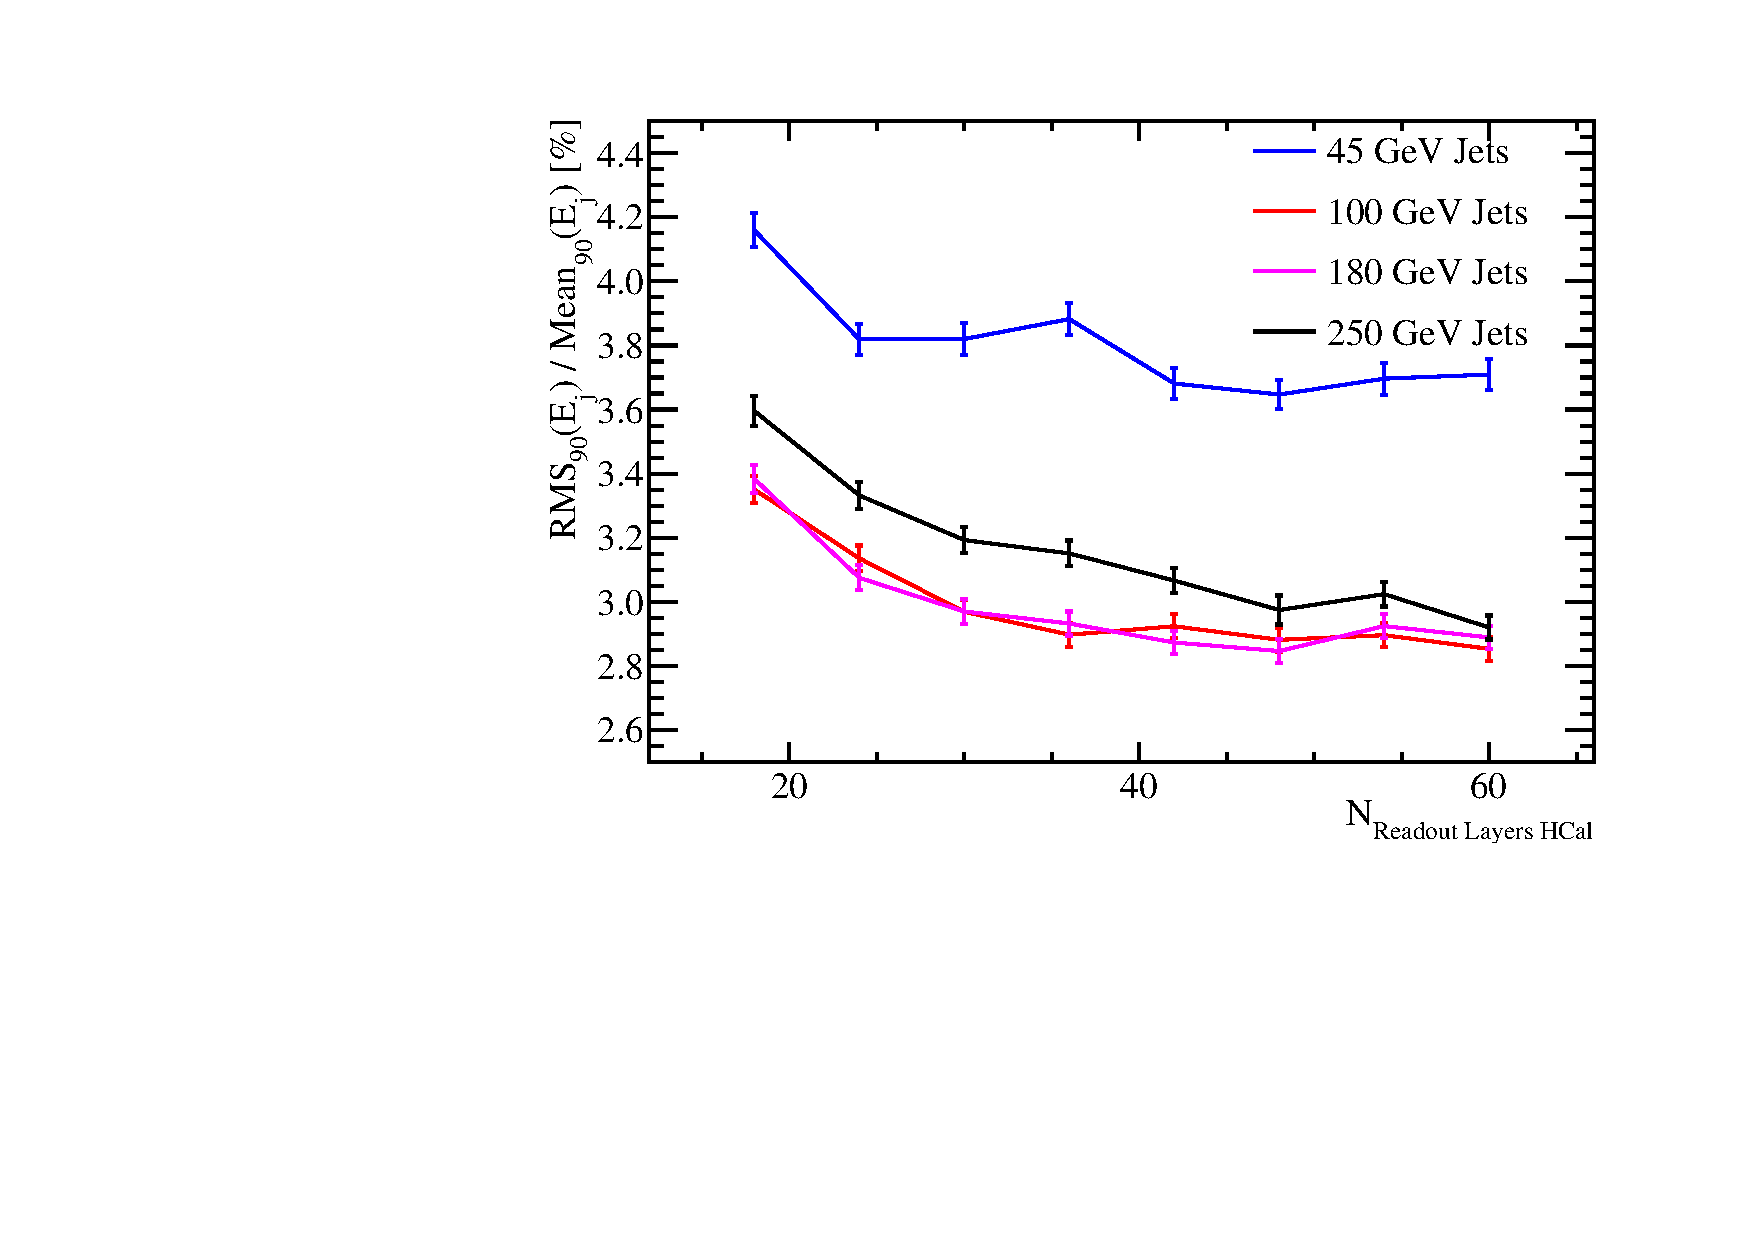
\includegraphics[width=0.5\textwidth]{OptimisationStudies/Plots/JetEnergyResolutions/JER_vs_NumberOfLayersInTheHCal.pdf}
\caption[Jet energy resolution as a function of longitudinal granularity in the HCal.]{Jet energy resolution as a function of longitudinal granularity in the HCal.}
\label{fig:hcalnlayers}
\end{figure}

The jet energy resolution for the various detector models considered is shown in figure \ref{fig:hcalnlayers}.  It was found that increasing the number of layers in the HCal, for the same total thickness, improved the jet energy resolution for all jet energies considered.  Based on the increase in the frequency of sampling of particle showers in the HCal, it is expected that the intrinsic energy resolution of the detector should improve.  However, the improvement observed in jet energy resolution for high energy jets indicates that longitudinal granularity is also affecting the confusion terms.

\begin{figure}
\centering
\subfloat[45 GeV Jets.]{\label{fig:hcalnlayers45break}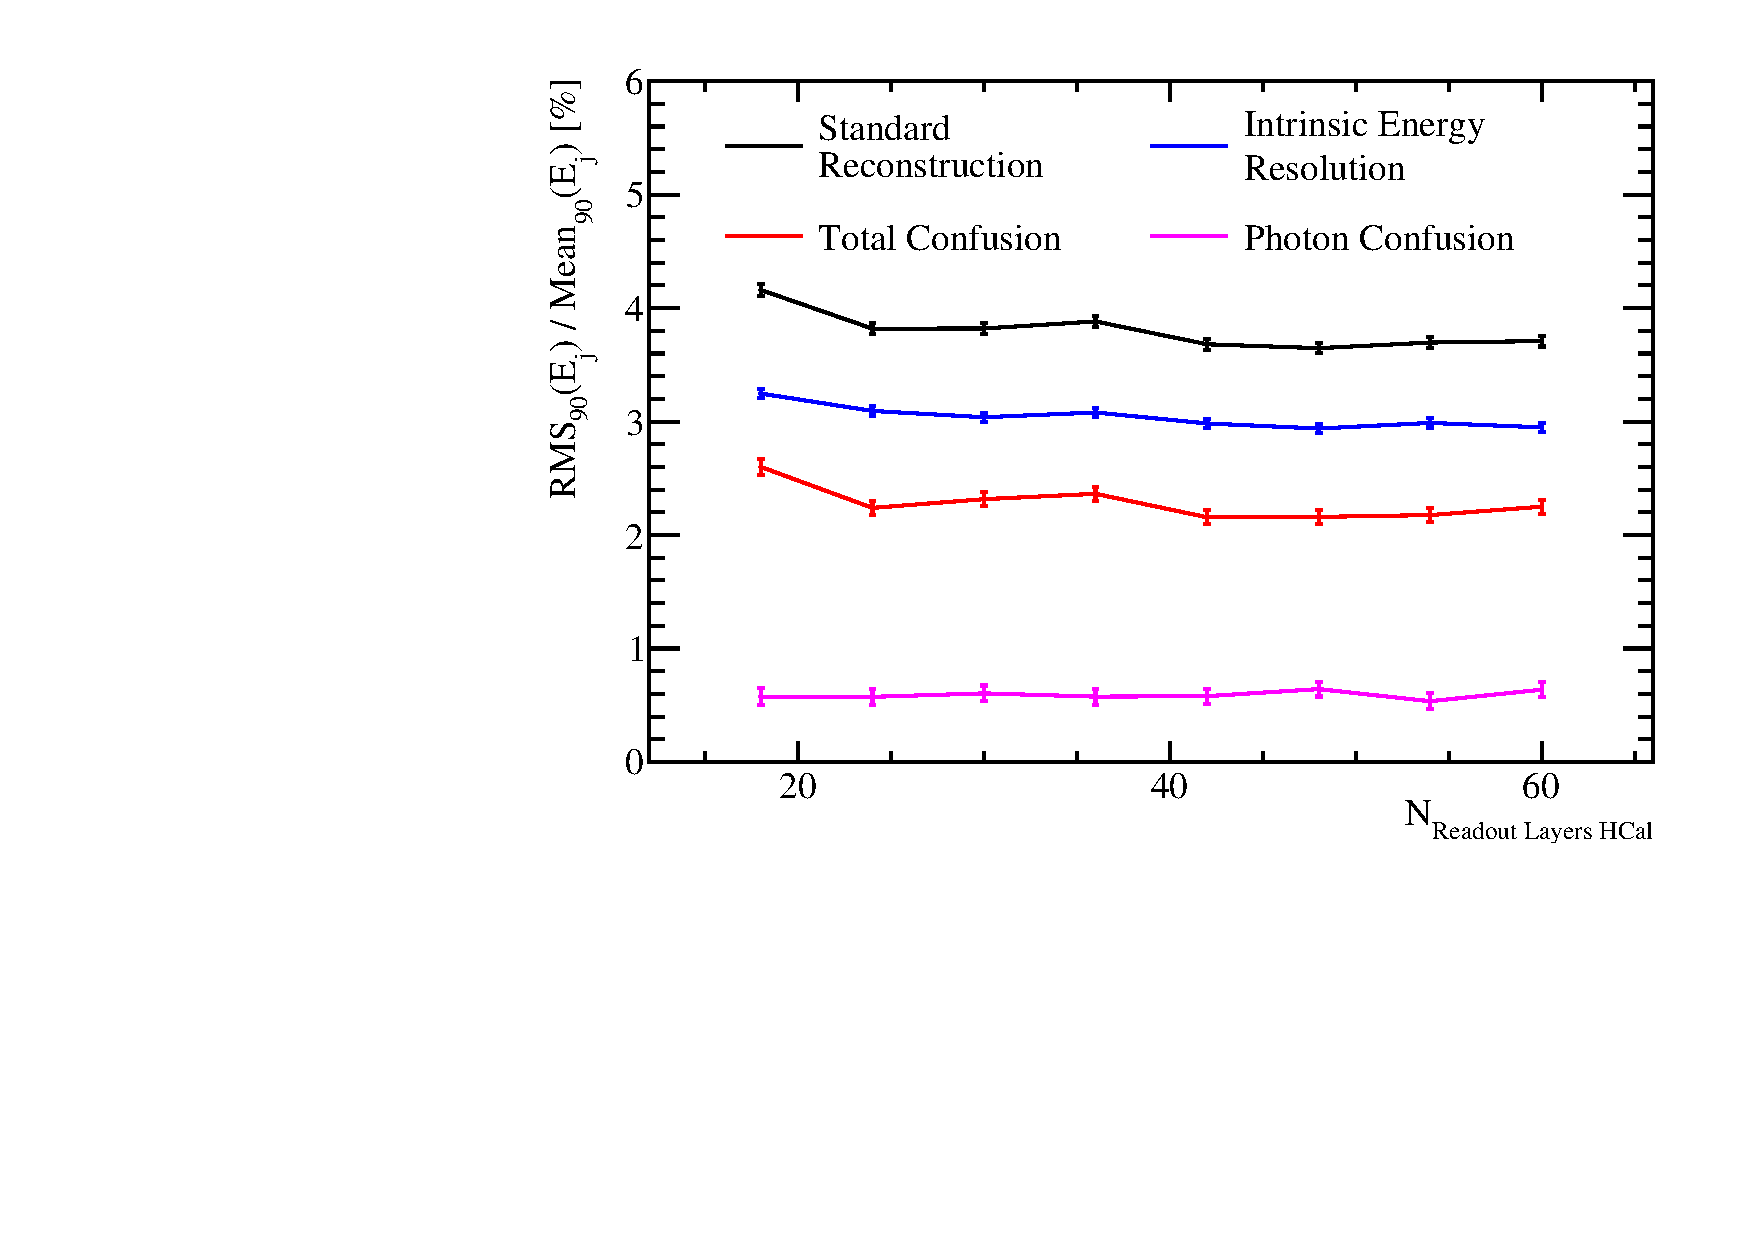
\includegraphics[width=0.5\textwidth]{OptimisationStudies/Plots/JetEnergyResolutions/JER_vs_NumberOfLayersInTheHCal_91GeV_DiJet_Breakdown.pdf}}
\subfloat[250 GeV Jets.]{\label{fig:hcalnlayers250break}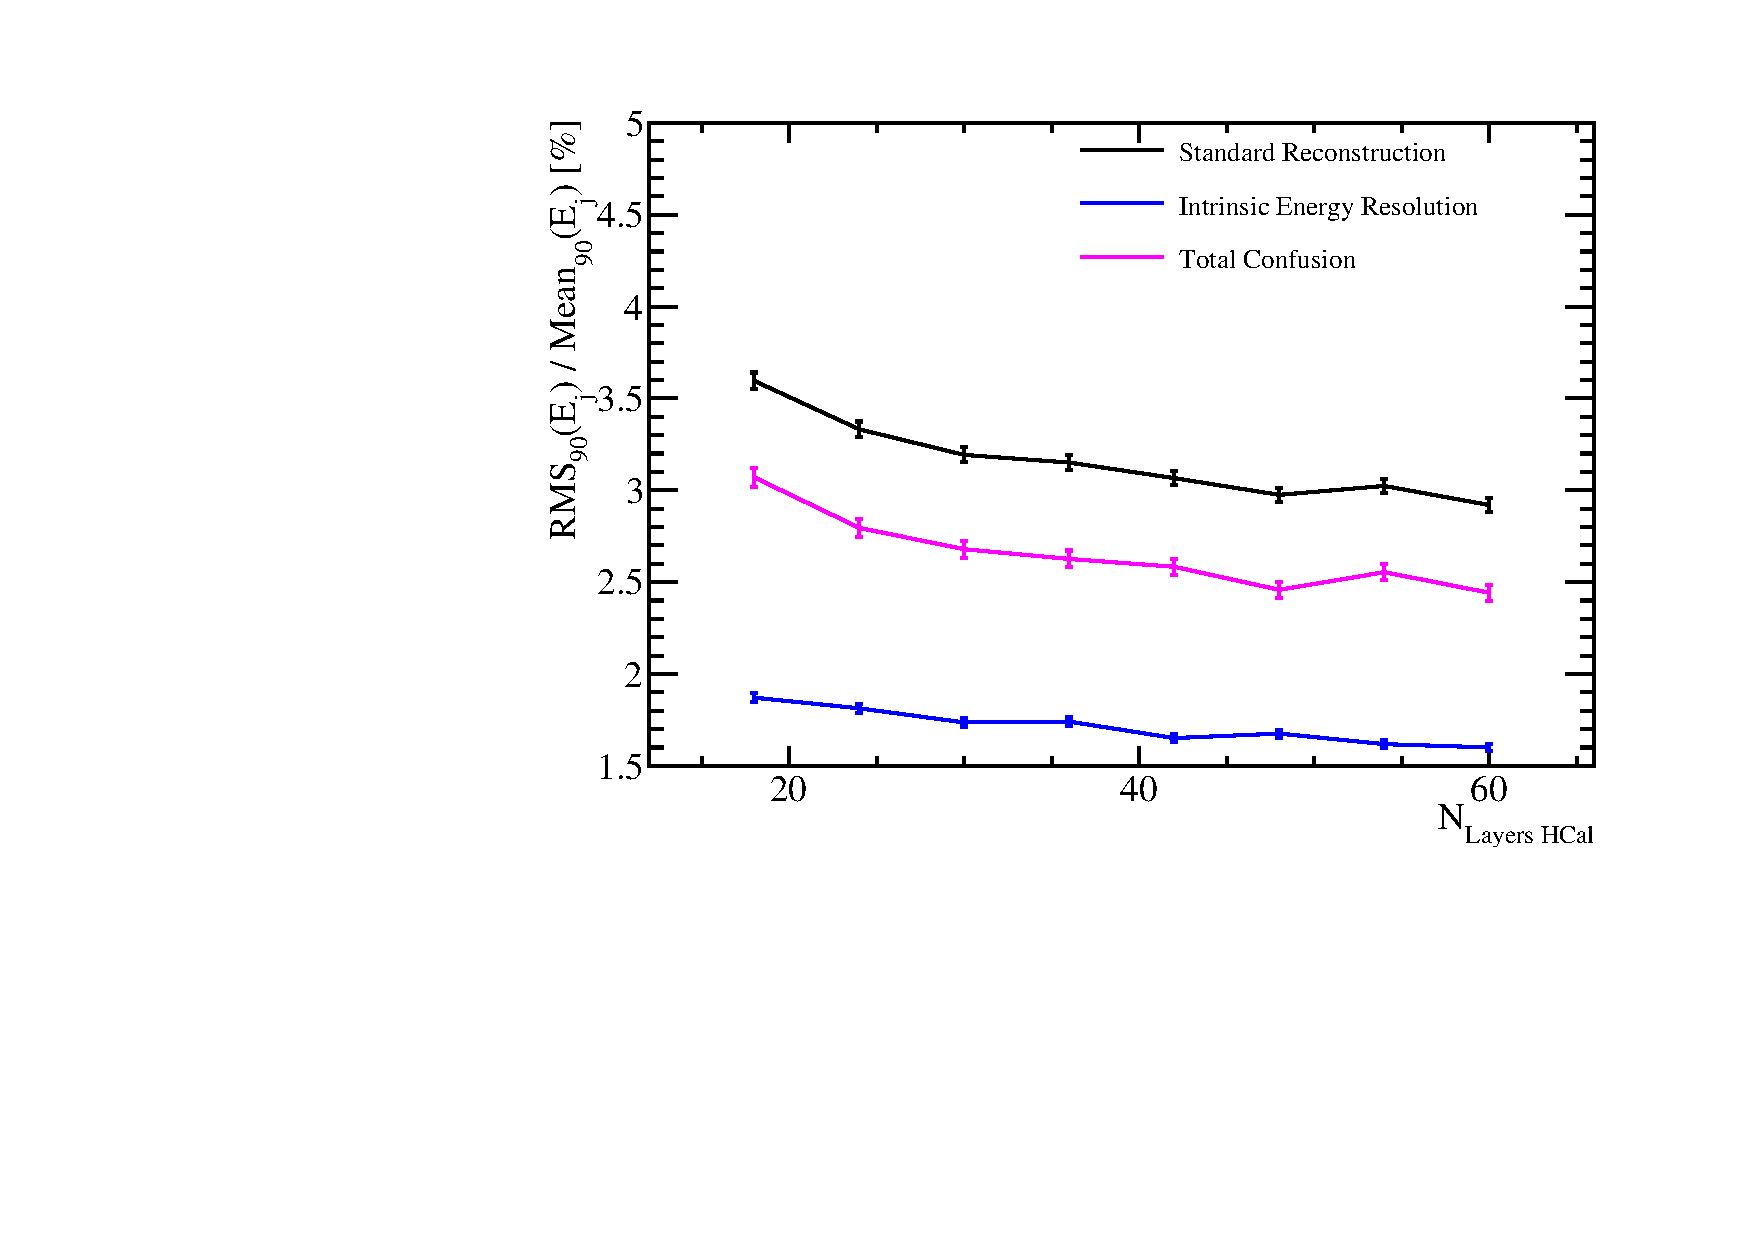
\includegraphics[width=0.5\textwidth]{OptimisationStudies/Plots/JetEnergyResolutions/JER_vs_NumberOfLayersInTheHCal_500GeV_DiJet_Breakdown.pdf}}
\caption[Jet energy resolution breakdown as a function of HCal longitudinal granularity for 45 and 250 GeV jets.]{Jet energy resolution breakdown as a function of HCal longitudinal granularity for 45 and 250 GeV jets.}
\label{fig:hcalnlayersbreak}
\end{figure}

These trends are further explored by considering the breakdown of jet energy resolution, which are shown in figure \ref{fig:hcalnlayersbreak}.  As expected from the standard performance reconstruction trends as a function of jet energy, there is an improvement in both the intrinsic energy resolution and a reduction in the impact of confusion when the number of layers in the HCal is increased.  The dominant trend driving the overall detector performance is that associated with the confusion of separating energy deposits from charged and neutral particles.  This emphasises the importance of pattern recognition to detector performance in the particle flow paradigm.    

\begin{figure}
\centering
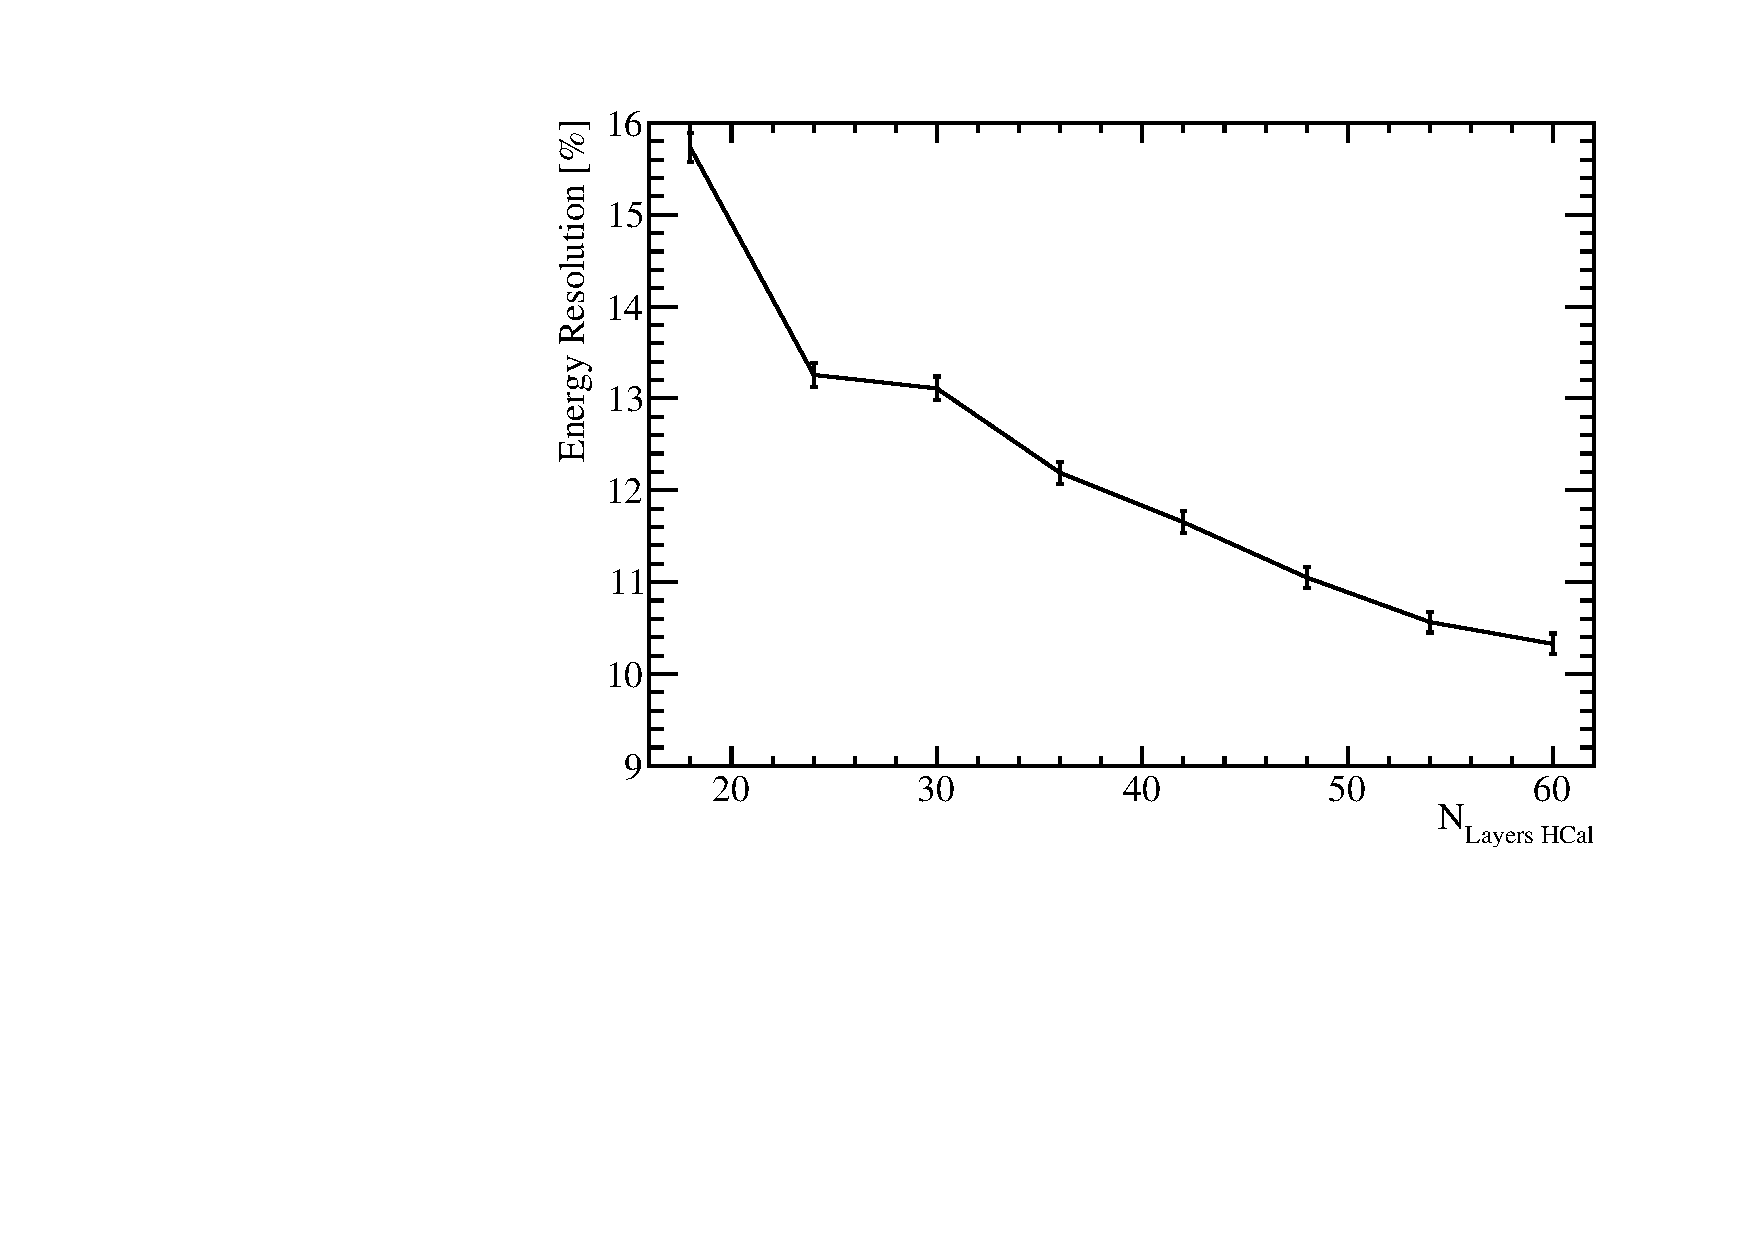
\includegraphics[width=0.5\textwidth]{OptimisationStudies/Plots/EnergyResolution/ER_vs_HCalLayerNumber_50GeVKaon0L.pdf}
\caption[Energy resolution as a function of HCal longitudinal granularity for 50 GeV $\text{K}^{0}_{L}$.]{Energy resolution as a function of HCal longitudinal granularity for 50 GeV $\text{K}^{0}_{L}$.}
\label{fig:hcalnlayers}
\end{figure}

The change in the intrinsic energy resolution of the HCal when varying the longitudinal granularity is best summarised by looking at the energy resolution of neutral hadrons as in the particle flow paradigm the energy of neutral hadrons is primarily measured in the HCal.  A plot of energy resolution against the number of layers in the HCal for 50 GeV $\text{K}^{0}_{L}$ can be found in figure \ref{fig:hcalnlayers}.  This data shows that a reduction in sampling frequency of a particle shower that accompanies a reduction in the number of readout layers results in a broadening of energy distributions and a degradation in the resolution.  It should again be emphasised that these results are for the full ILD detector model and so include the effect of the $\approx 1 \lambda_{I}$ in the ECal.  

The increasing the HCal longitudinal granularity has a twofold effect on the detector performance: an increase in sampling rate of particle showers and an improvement to the intrinsic energy resolution and a reduction in the confusion arising from associating energy deposits from hadrons.  

%========================================================================================
%========================================================================================

\section{Global Detector Parameters}


\iffalse
\label{optstud:sec:hcal:nlayers}


\begin{figure}
  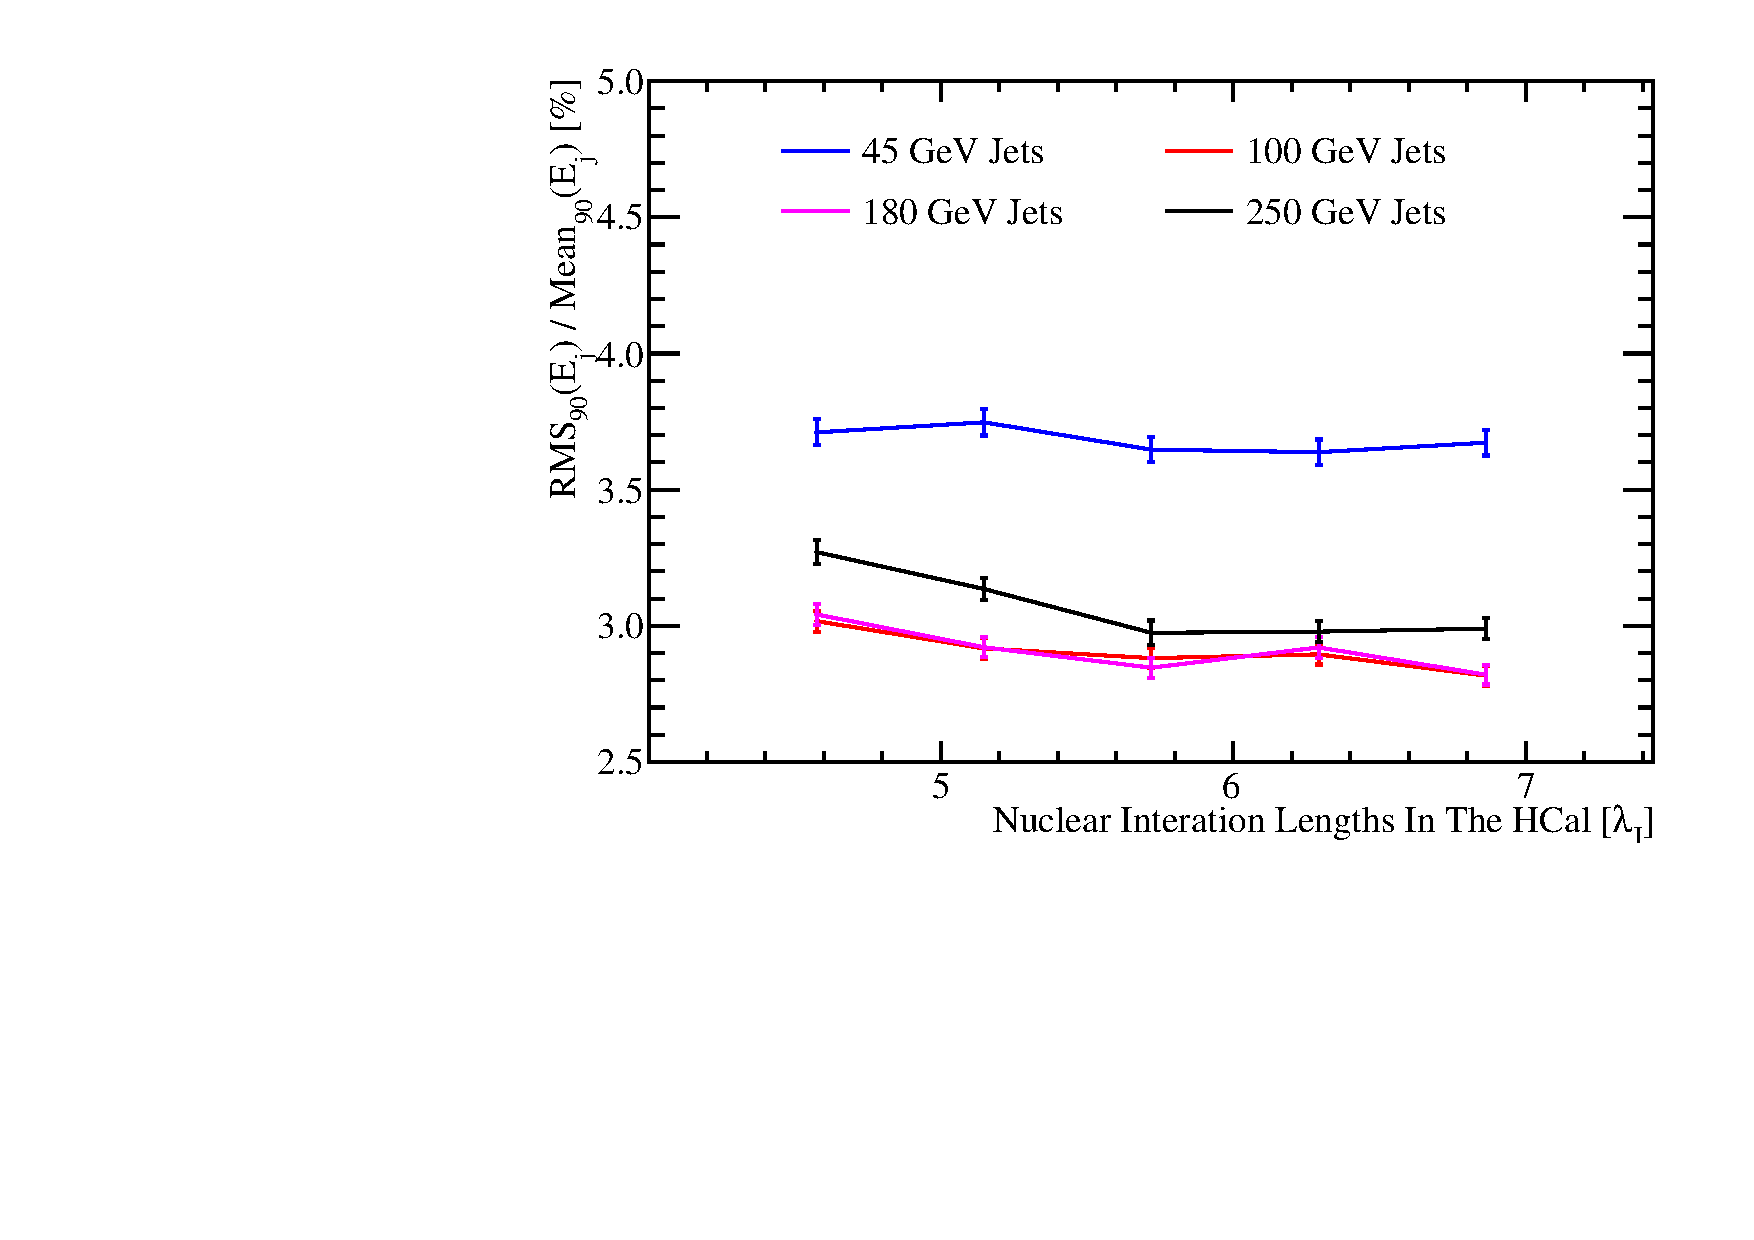
\includegraphics[width=0.5\textwidth]{OptimisationStudies/Plots/JetEnergyResolutions/JER_vs_NumberOfNuclearInterationLengthsInTheHCal.pdf}
  \caption[Jet energy resolution as a function of the number of nuclear interaction lengths in the HCal for the scintillator steel HCal option.]{Jet energy resolution is shown for several fixed energy jets as a function of the number of nuclear interation lenghts in the HCal for the scintillator steel HCal option.}
  \label{optstud:fig:hcaldepth}
\end{figure}

\begin{figure}
  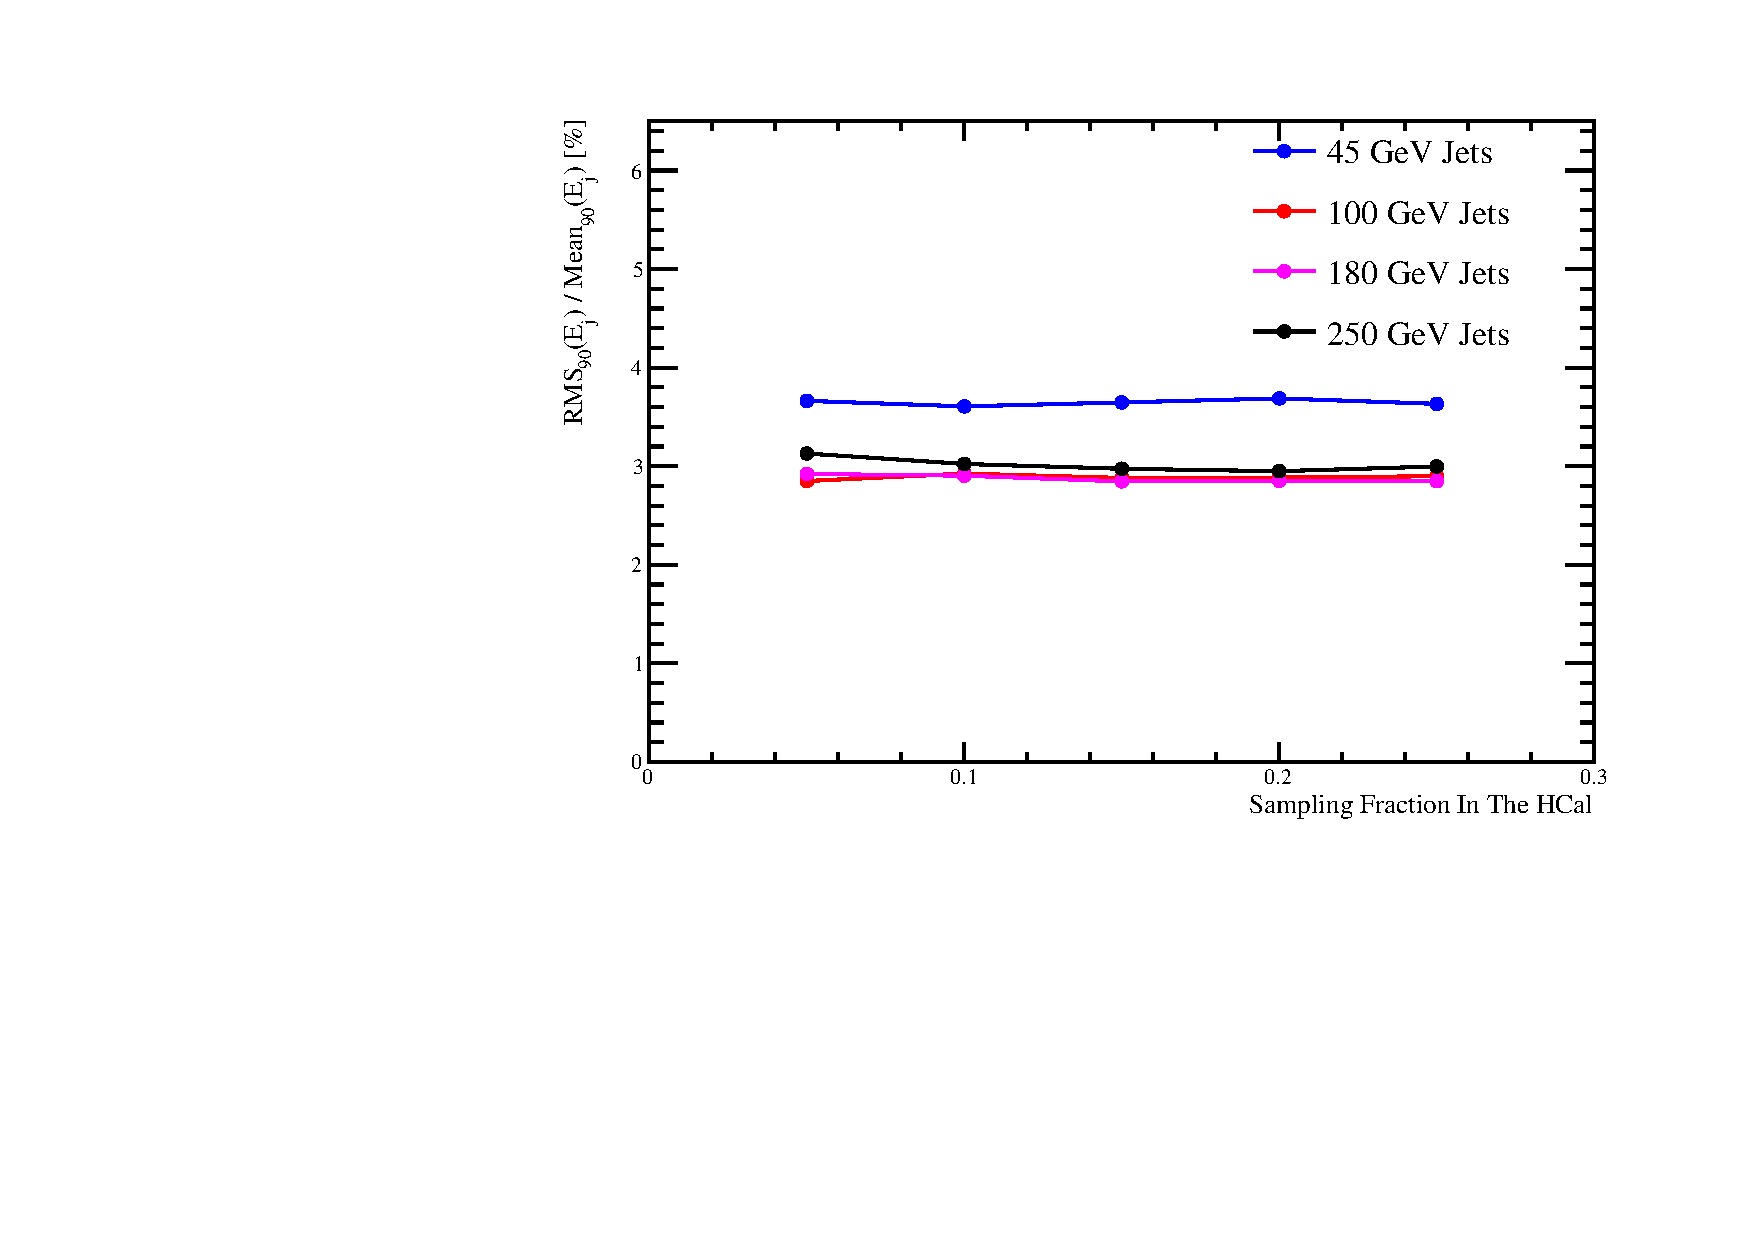
\includegraphics[width=0.5\textwidth]{OptimisationStudies/Plots/JetEnergyResolutions/JER_vs_SamplingFractionInTheHCal.pdf}
  \caption[Jet energy resolution as a function of the sampling fraction in the HCal for the scintillator steel HCal option.]{Jet energy resolution is shown for several fixed energy jets as a function of the sampling fraction in the HCal for the scintillator steel HCal option.}
  \label{optstud:fig:hcalsampfrac}
\end{figure}

\subsection{HCal Absorber Material}
\label{optstud:sec:hcal:absmat}

\begin{figure}
  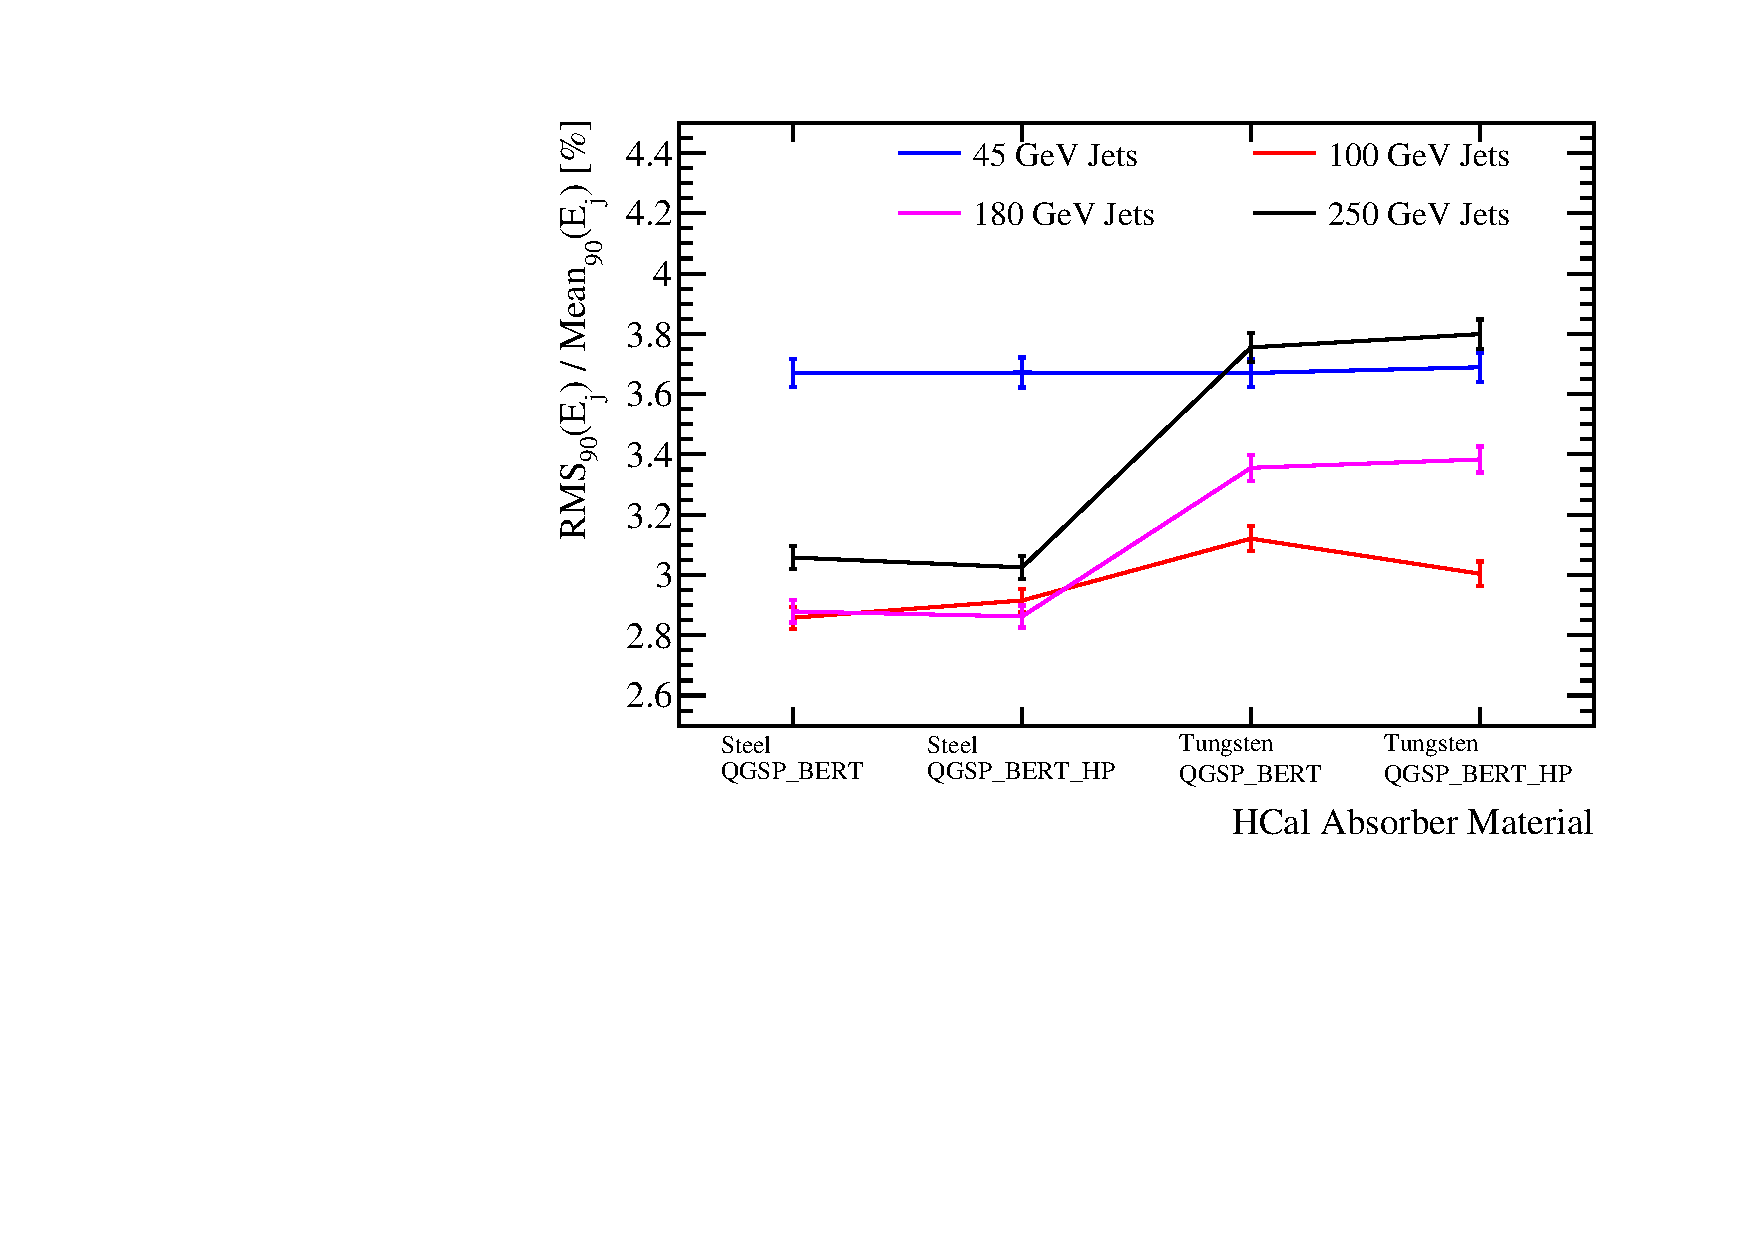
\includegraphics[width=0.5\textwidth]{OptimisationStudies/Plots/JetEnergyResolutions/JER_vs_HCalAbsorberMaterial.pdf}
  \caption[Jet energy resolution as a function of the absorber matieral in the HCal.]{Jet energy resolution is shown for several fixed energy jets as a function of the absorber material in the HCal.}
  \label{optstud:fig:hcalabsmat}
\end{figure}

\section{Global Detector Parameter Optimisation}
\label{optstud:sec:global}

\subsection{Magnetic Field Strength}
\label{optstud:sec:glob:bfield}

\begin{figure}
  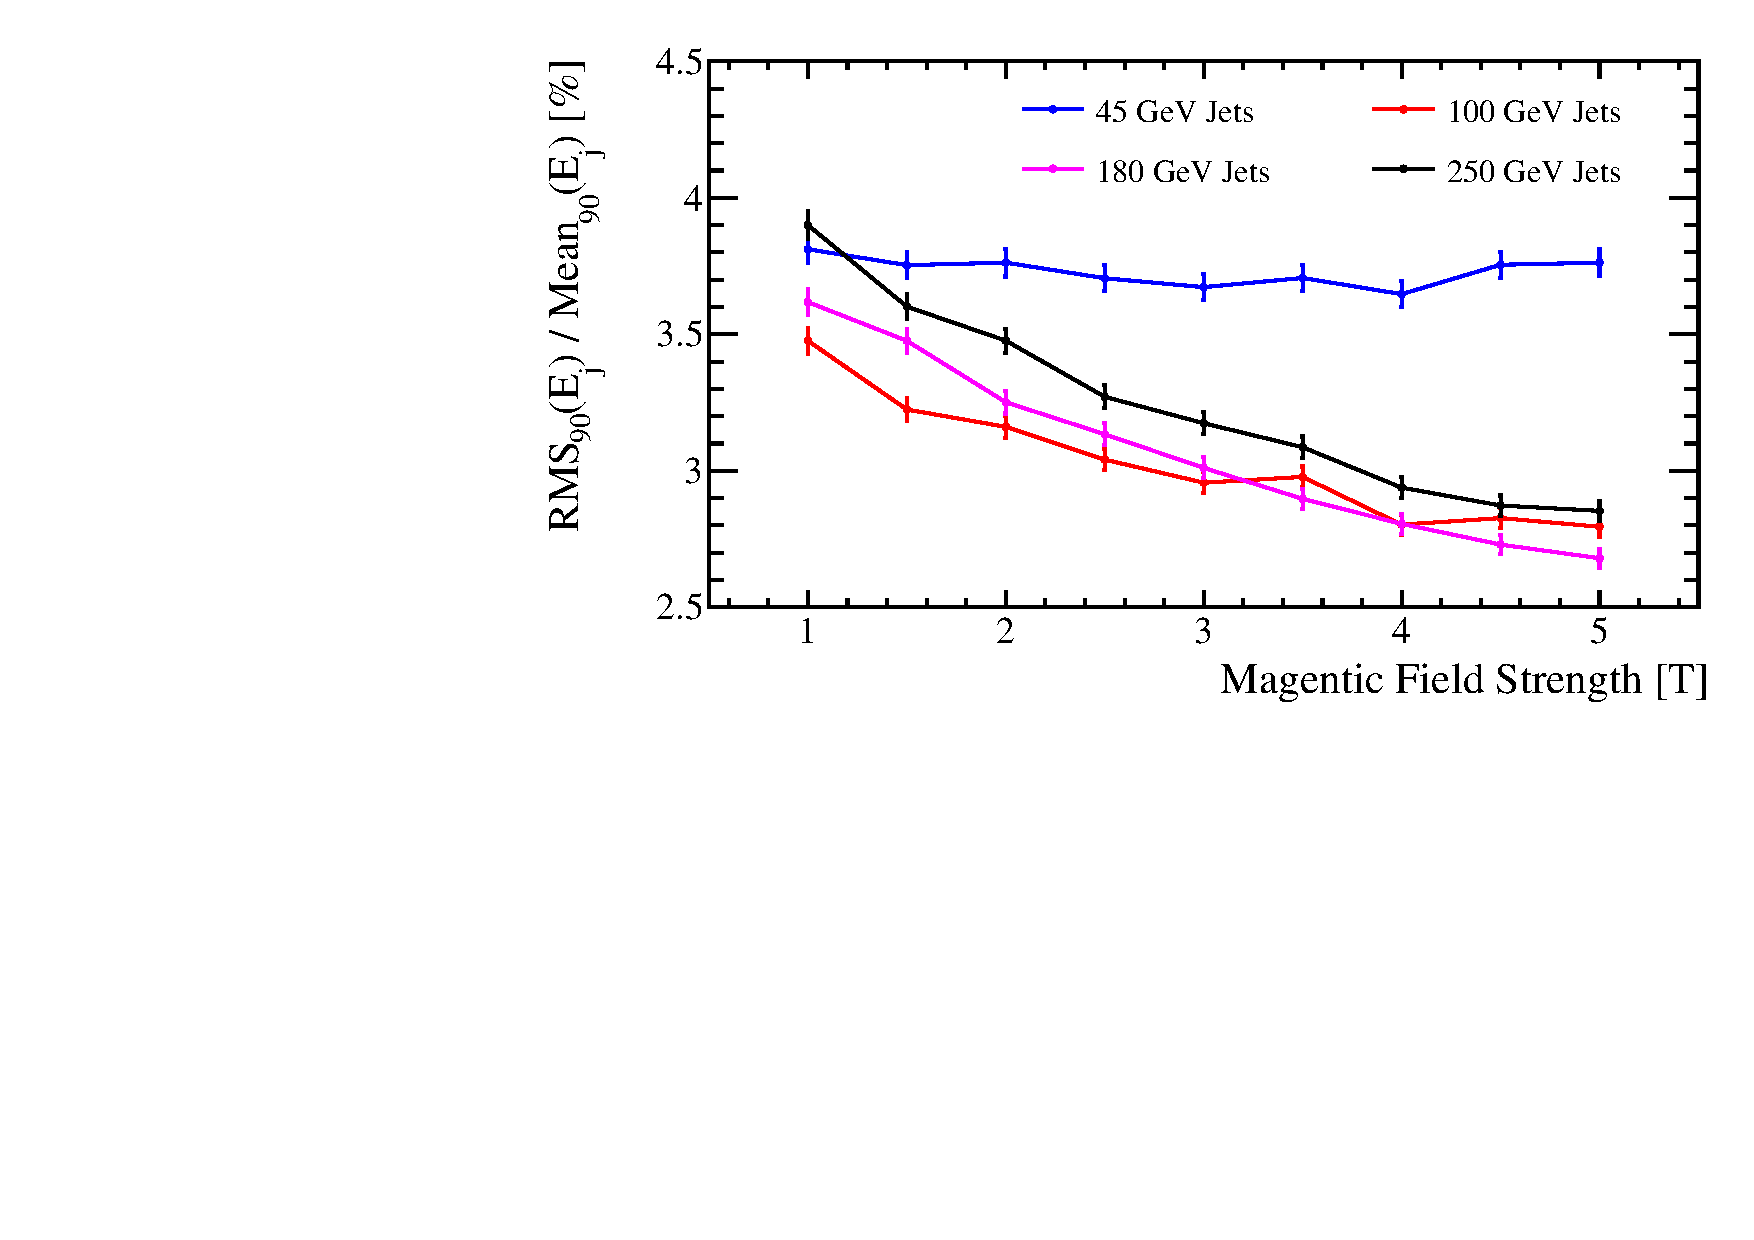
\includegraphics[width=0.5\textwidth]{OptimisationStudies/Plots/JetEnergyResolutions/JER_vs_MagneticField.pdf}
  \caption[Jet energy resolution as a function of magnetic field strength.]{Jet energy resolution is shown for several fixed energy jets as a function of magetic field strength.}
  \label{optstud:fig:bfield}
\end{figure}

\subsection{Inner ECal Radius}
\label{optstud:sec:glob:ecalinnerrad}

\begin{figure}
  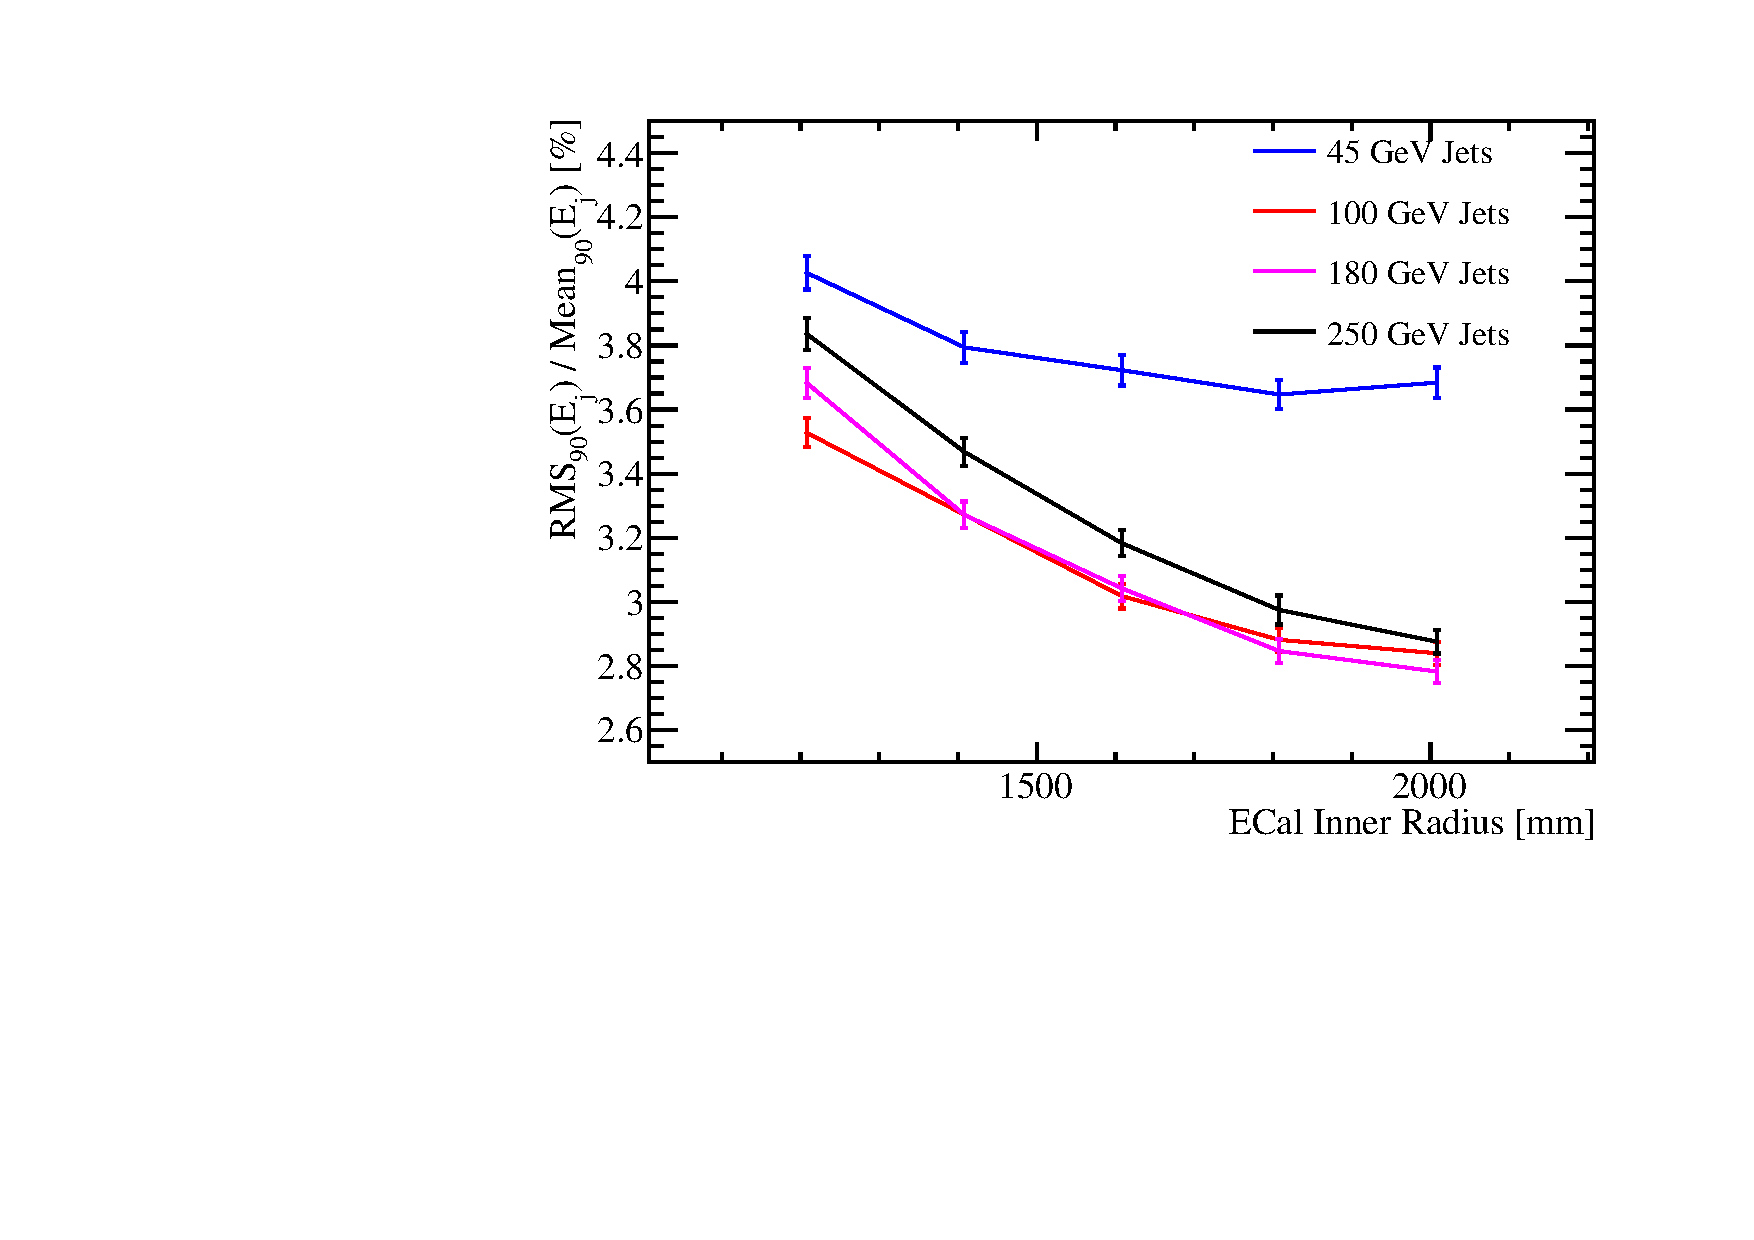
\includegraphics[width=0.5\textwidth]{OptimisationStudies/Plots/JetEnergyResolutions/JER_vs_ECalInnerRadius.pdf}
  \caption[Jet energy resolution as a function of the ECal inner radius.]{Jet energy resolution is shown for several fixed energy jets as a function of the inner ECal radius.}
  \label{optstud:fig:ecalinnerrad}
\end{figure}

\fi

\iffalse
JER_vs_BothECalCellSize.C                                   JER_vs_MagneticFieldStrength.C                              JER_vs_ScintillatorECalCellSize_91GeV_DiJet_Breakdown.pdf
JER_vs_BothECalNumberofLayers.C                             JER_vs_MagneticFieldStrength.pdf                            JER_vs_ScintillatorECalNumberofLayers.C
JER_vs_ECalInnerRadius.C                                    JER_vs_NumberOfLayersInTheHCal.C                            JER_vs_ScintillatorECalNumberofLayers.pdf
JER_vs_ECalInnerRadius.pdf                                  JER_vs_NumberOfLayersInTheHCal.pdf                          JER_vs_SiliconECalCellSize.C
JER_vs_HCalAbsorberMaterial.C                               JER_vs_NumberOfNuclearInterationLengthsInTheHCal.C          JER_vs_SiliconECalCellSize.pdf
JER_vs_HCalAbsorberMaterial.pdf                             JER_vs_NumberOfNuclearInterationLengthsInTheHCal.pdf        JER_vs_SiliconECalCellSize_500GeV_DiJet_Breakdown.C
JER_vs_HCalCellSize.C                                       JER_vs_SamplingFractionInTheHCal.C                          JER_vs_SiliconECalCellSize_500GeV_DiJet_Breakdown.pdf
JER_vs_HCalCellSize.pdf                                     JER_vs_SamplingFractionInTheHCal.pdf                        JER_vs_SiliconECalCellSize_91GeV_DiJet_Breakdown.C
JER_vs_HCalCellSize1000000GeVMHHHE.C                        JER_vs_ScintillatorECalCellSize.C                           JER_vs_SiliconECalCellSize_91GeV_DiJet_Breakdown.pdf
JER_vs_HCalCellSize1000000GeVMHHHE.pdf                      JER_vs_ScintillatorECalCellSize.pdf                         JER_vs_SiliconECalNumberofLayers.C
JER_vs_HCalCellSize1GeVMHHHE.C                              JER_vs_ScintillatorECalCellSize_500GeV_DiJet_Breakdown.C    JER_vs_SiliconECalNumberofLayers.pdf
JER_vs_HCalCellSize1GeVMHHHE.pdf                            JER_vs_ScintillatorECalCellSize_500GeV_DiJet_Breakdown.pdf  
JER_vs_MagneticField.pdf                                    JER_vs_ScintillatorECalCellSize_91GeV_DiJet_Breakdown.C 
\fi


